% !Mode:: "TeX:UTF-8:Hard"

\documentclass[a4paper,11pt,twoside]{book}
%\usepackage{CJKutf8}
\usepackage[T1]{fontenc}
\usepackage{pifont}
\usepackage{graphicx}
\usepackage{multirow} 
\usepackage{longtable}
\usepackage{capt-of}
\usepackage{color}
\usepackage{amsmath}
\usepackage{enumitem}

\setitemize[1]{itemsep=0pt,partopsep=0pt,parsep=1pt,topsep=0pt}
\setenumerate[1]{itemsep=0pt,partopsep=0pt,parsep=1pt,topsep=0pt}
\setdescription{itemsep=0pt,partopsep=0pt,parsep=1pt,topsep=0pt}

\usepackage[a4paper,left=2cm,right=2cm,top=3cm,bottom=3cm,]{geometry}

\newcommand{\linuxcommand}[1]{\texttt{\textcolor{blue}{\$ #1 \Pisymbol{psy}{191}}}}
\newcommand{\op}[1]{\textcolor{blue}{-#1}}
\newcommand{\hotkey}[1]{\framebox{#1}}
\newenvironment{screen}{\sffamily}{\rmfamily}

% for C/C++ frame box
\usepackage{listings}
\definecolor{mygray}{rgb}{0.9,0.9,0.9}

\lstset{ 
	backgroundcolor=\color{mygray},
	mathescape=true,
	frame=single,
	frameround=tttt,
	language=c++,
	basicstyle=\footnotesize,
	%literate={\ \ }{{\ }}1
	tabsize=2,
	numbersep=6pt,
	breaklines=true,
	%framextopmargin=0.5em,
	%framexbottommargin=0.5em,
	morecomment=[s][\color{red}]{/*-}{*/},
	%escapeinside={//*}{*//},
	numberstyle=\tiny\textit,  stepnumber=1,
	numbers=left,
}

\lstset{morecomment=[s][\color{red}]{/*-}{*/}}
\newcommand{\Hilight}[1]{\makebox[0pt][l]{\color{yellow}\rule[-3pt]{#1em}{11pt}}}
\newcommand{\HilightLine}[2][yellow]{\makebox[0pt][l]{\color{#1}\rule[-4pt]{#2em}{13.9pt}}}

\newenvironment{answer}{\ttfamily}{\par}

\newcommand{\specialcell}[2][c]{%
  \begin{tabular}[#1]{@{}c@{}}#2\end{tabular}}

\begin{document}
%\begin{CJK*}{UTF8}{song}
\title{Data Structure and Algorithm}
\author{yan zhao}
\date{}\maketitle

\setcounter{secnumdepth}{4}
\setcounter{tocdepth}{4}
\tableofcontents

\setlength\parindent{0pt}
\setlength{\parskip}{5pt}

\chapter{Data structure} 

	\par Data structure is known as ADT (Abstract Date Type),  which is independent of implementation. For example, stack can be implemented by array or linked list inside. Such as stack in STL library, It's implemented by \texttt{std::deque} default.   
	
	\par \textbf{Linear and hierarchical structures}. Array, linked lists, stacks and queue are linear structures. And tree, graph, heaps are hierarchical.
	
	\par STL is a good reference when you learn data structure, especially (API) design and interface of STL container. such as \texttt{push}, \texttt{pop}  and \texttt{top} for \texttt{stack} and \texttt{priority\_queue}. For \texttt{queue}, besides \texttt{push, pop},  there are also \texttt{front()} and \texttt{back()}. Just remember five words: \textbf{push, pop, front, back and top}.
	
\section{Array}

\subsection{Basic operation of array}

	All language support array and it is a build-in data type in most of language.  
\begin{lstlisting}[frame=single, language=c++]
//C/C++ language
int a[3]; or int a[4][5].  
vector<int> vi(4,0); //STL
array<int, 4> al = {1, 2, 3 , 4}; //new array in STL
  
//C# language 
object[] a1 = {"string", 123, true};
\end{lstlisting}

	\par Array support three basic operations: random access (index), insert, erase.  

	\par Dynamic two dimension array (ragged array) can be implemented below:  \texttt{char ** p;}. Pay attention to \texttt{p[1][2]} and \texttt{pa[1][2]} in the below code. They are all correct forms.

	\par All ragged array should include terminate flag, so you can know the length of each row.  For C-style string ragged array, the 'NULL' in the end of string can be used as terminate flag directly, so ragged array is idea container for C-style string array. 

\begin{lstlisting}[frame=single, language=c++]
char **p;
char* a[]={"zhao","yan","hello"}; 
p = a;    // use pointer of pointer to catch array of pointer.
printf("%c\n",*(*(p+1)+2)); //p[1][2]

int (*pa)[3];  //pointer to array.
int aa[2][3] = {{1,2,3},{4,5,6}};
pa = aa;
int bb[][3]; //bb must have 3 as last dimension. c++ syntax.
bb = aa;
printf("%d\n",pa[1][2]);//*(*(pa+1)+2);
\end{lstlisting} 
\begin{description}
	\item[line 7-10] this is array of \textbf{array}. so you have to use \textbf{a pointer to array} to catch it. Pay attention to the syntax of a pointer to array in C++ language: \texttt{int (*pointer\_to\_array)[3];}
\end{description}




	\par If you have an array of big object, and you need to sort it. You can build a array of pointer to point to each object in the array. When you sort the an array of big object,  you just move pointer instead, It is called \textbf{"indirect addressing"}, It can help you to avoid moving big chunk of data.  


	\par If you want to insert an element into an array, you  \textbf{need to copy backward from end. }
if erase an element from an array, \textbf{copy forward from erasing point}. Most of time, you can just call insert(pos) or erase(pos) in STL container. \textbf{It inserts the element before the pos and erase the element at th pos}, and pos is an iterator.  

\begin{center}
	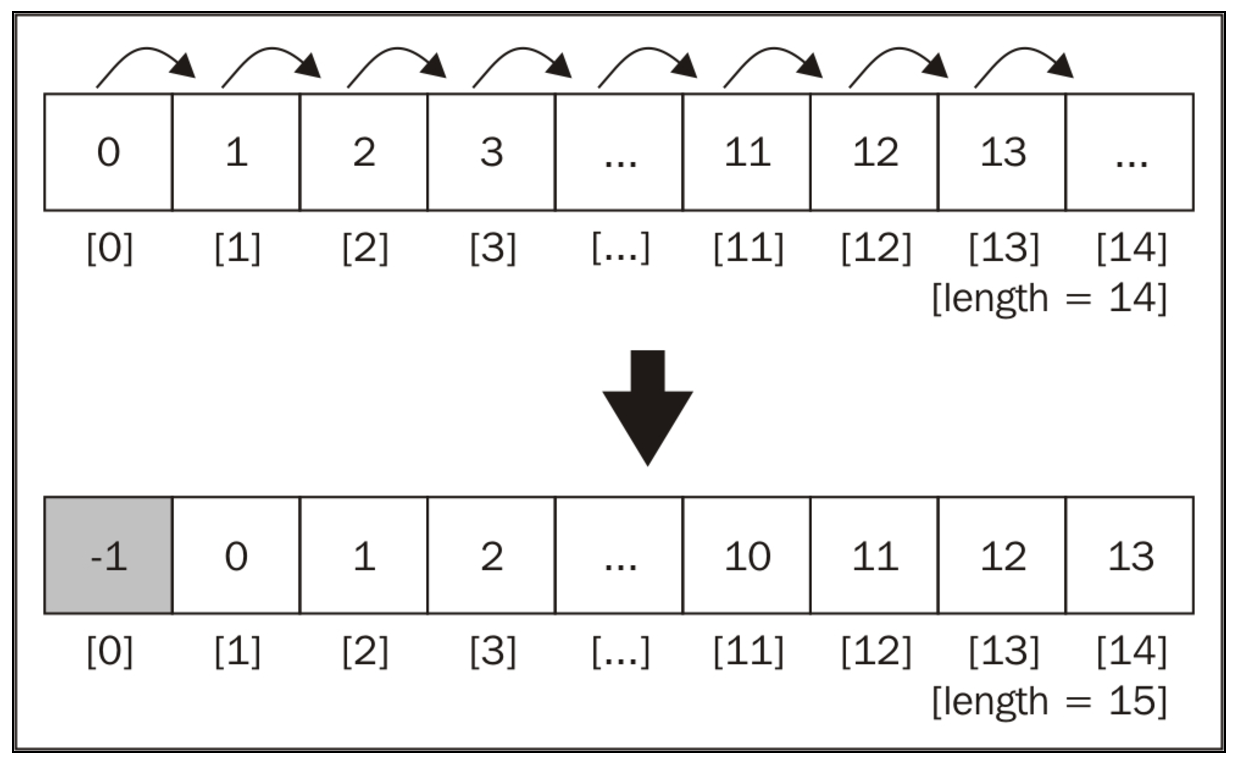
\includegraphics[scale=0.35]{pics/array_insert.png} 
\end{center}


	
	\par  Reverse array can be implemented by \textbf{swap + double pointers}, But reversing list need different algorithm, so in STL , \texttt{std::list} has its own reverse member function. Reverse list is a typical interview question, and you should know it very well. 
	
	\par Boundary about array structure. 
	\begin{itemize}
		\item Remember: if \texttt{n} is size of array, \texttt{n/2} is the middle element (odd) or the first element in the second half (even). This pattern is very helpful for you to write reverse function. 
		
		\item Remember: if \texttt{end} is end of index, \texttt{end/2} is the middle element (odd) or the last element in the first half(even). Be careful with this, most of time, D\&C like to use start and end index, not size of array. 
		
		\item \texttt{std::distance(v.begin(), v.end());} is size of array/vector. 
	\end{itemize}
	
\begin{lstlisting}[breaklines]
void reverseArray(int a [], int n){
	int i,j,temp;
	for(i=0,j=n-1;i<n/2;++i,--j){
		swap(a[i], a[j]);
	}
}

//another is based on iterator
for(auto i = v.begin() auto j = v.end()-1; i<next(i, distance(v.begin(), v.end())/2) ; ++i, --j)
	iter_swap(i,j);

//pay attention next and distance usage, put being in front of end.
//distance(v.end(), v.begin()) is just size of array/vector. 
\end{lstlisting}

	\par  Write a function rotate(ar[], d, n) that rotates arr[] of size n by d elements.
\begin{itemize}
	
	\item Single rotate method
\begin{lstlisting}[breaklines]
while(d-- >0 ){ //d-- >0 is good trick
  int temp = Array[0];
  for (int i = 0; i < n-1; i++){
    Array[i] = Array[i + 1];
  }
  Array[n-1] = temp;
}
\end{lstlisting}

	\item Reverse method. That is a very efficient implementation.
\begin{lstlisting}[breaklines]
rotate(arr[], d, n)
  reverse(arr[], 1, d) ;
  reverse(arr[], d + 1, n);
  reverse(arr[], l, n);
\end{lstlisting}
\textbf{Idea: middle part reverse twice, so keep origin value}

	\item For \texttt{std::list}, you can use \texttt{std::rotate}, but the time complexity is O(n), you can use splice function to reach O(1).  
\begin{lstlisting}
std::list l{1, 2, 3, 4, 5};
auto i2 = std::next(i1, 2);

l.splice(l.end(), l, l.begin(), i2 ); //output 3, 4, 5, 1, 2
\end{lstlisting}


	\item You can use \texttt{std::rotate} in insert sort method. It also can be used in slide. Detail can be found in "Top 5 Beautiful C++ std Algorithms Examples"
\begin{lstlisting}[breaklines, basicstyle=\scriptsize]
for (auto i = start; i != end; ++i)
	std::rotate(std::upper_bound(start, i, *i), i, std::next(i));  
	//all stl algorithms deal with left close, right open space. 
	//i and std::next(i) is right open point.

template <typename It> 
auto slide(It f, It l, randIter p) -> std::pair<It, It>{
  //  p < [f...l] < p, two possibles 
  if (p < f) return { p, std::rotate(p, f, l) };
  if (l < p) return { std::rotate(f, l, p), p };
  return { f, l };
}

ForwardIt rotate( ForwardIt first, ForwardIt n_first, ForwardIt last );
// rotate returns Iterator to the new location of the element pointed by first
\end{lstlisting}
\begin{description}
	\item[line 2:] rotate(a, b, c) is [a,b) and [b,c) scope. they are all left close, right open scope. In this way, you can understand why we need \texttt{std::next(i)} here.
\end{description}

	\item You need to remember below code snippet. \textbf{reverse-->rotate--> insertion order and slide}. 

\end{itemize}

	\par  We can also use partition to implement gather. \textbf{Partition return: Iterator to the first element of the second group.}

	\par  Gather all eligible element around iterator p
\begin{lstlisting}[numbers=none]
template <typename BiIt, typename UnPred> 
auto gather(BiIt f, BiIt l, BiIt p, UnPred s) -> std::pair <BiIt, BiIt>{
	return { stable_partition(f, p, not1(s)), 
		stable_partition(p, l, s) };
}		
\end{lstlisting}





\subsection{Interview questions}
\begin{itemize}
	\item Two sum. 
\begin{enumerate}
\item Answer 1: First Sort O(n*log(n)), then use two pointers.
\begin{lstlisting}[tabsize=3]
bool hasArrayTwoCandidates(int A[], int arr_size, int sum) { 
	int l, r; 
	sort(A, A + arr_size); 
	
	/* Now look for the two candidates in  the sorted array*/
	l = 0; 
	r = arr_size - 1; 
	while (l < r) { 
		if (A[l] + A[r] == sum) 
			return 1; 
		else if (A[l] + A[r] < sum) 
			l++; 
		else // A[i] + A[j] > sum 
			r--; 
	} 
	return 0; 
} 
\end{lstlisting}
\textbf{Idea: Don't need keep index information, so you can sort it. }

\item Answer 2: Hash O(n)
\end{enumerate}

\item Count triplets with sum smaller than a given value. 
\begin{lstlisting}[breaklines]
1) Sort the input array in increasing order. 
2) Initialize result as 0.
3) Run a loop from i = 0 to n-2.  An iteration of this loop finds all
   triplets with arr[i] as first element.
     a) Initialize other two elements as corner elements of subarray 
        arr[i+1..n-1], i.e., j = i+1 and k = n-1
     b) Move j and k toward each other until they meet, i.e., while (j < k)
            (i) if (arr[i] + arr[j] + arr[k] >= sum), then do k-- 

            // Else for current i and j, there can (k-j) possible third elements that satisfy the constraint.
            (ii) Else Do ans += (k - j) followed by j++ 
\end{lstlisting}
\textbf{Idea: Same Idea as previous question, Don't need keep index information, so you can sort it. brutal force, only sort can help here.}


	\item Given an array of positive integers. All numbers occur even number of times except one number which occurs odd number of times. Find the number in O(n) time and constant space.
Example: I/P = [1, 2, 3, 2, 3, 1, 3] and O/P = 3. The Best Solution is to do bitwise XOR of all the elements. XOR of all elements gives us odd occurring element. Please note that XOR of two elements is 0 if both elements are same and XOR of a number x with 0 is x.

\begin{lstlisting}[breaklines]
	result = result ^ a[i];
\end{lstlisting}
\textbf{Idea: Perform some calculation on all elements. }


	\item You are given a list of n-1 integers and these integers are in the range of 1 to n. There are no duplicates in list. One of the integers is missing in the list. Write an efficient code to find the missing integer.
\begin{lstlisting}[breaklines]
1) Get the sum of numbers 
       total = n*(n+1)/2
2  Subtract all the numbers from total and you will get the missing number.
\end{lstlisting}
\textbf{Idea: Perform some calculation on all elements. }

	\item Max product of the three numbers for a given array of size N. \textbf{Find the three largest numbers in the array (n1, n2, n3) and the two smallest numbers (m1, m2). The answer is either n1 x n2 x n3 or n1 x m1 x m2. The tricky thing here is there are two potential answers.}
\begin{lstlisting}[breaklines]
nth_element(...)
\end{lstlisting}
\textbf{Idea: Not sort, but nth max element based on heap}

	\item Given an unsorted array of non-negative integers, find a \textbf{continuous} subarray which adds to a given number.  Examples: Input: arr[] = {1, 4, 20, 3, 10, 5}, sum = 33; Ouptut: Sum found between indexes 2 and 4. 

\begin{lstlisting}[breaklines]
int arr[] = {1, 4, 20, 3, 10, 5};
int left = 0; int right = 0;
int sum = 0;
while(right< 6){
	sum+=arr[right];
	++right;
	
	while(sum>33){
		sum-=arr[left];
		++left;
		if (sum == 33){
			cout<<left<<" "<<right<<" "<<endl;
		}
	}	
}
\end{lstlisting}
\textbf{Idea: 1) You must keep index information, so you can't sort. }  \textbf{That is a typical sliding window problems. Keep left and right two index. } Sliding window can be found in algorithm chapter. 

	\item Given an array \texttt{arr[]} of integers, find out the difference between any two elements such that larger element appears after the smaller number in arr[]. Examples: If array is [2, 3, 10, 6, 4, 8, 1] then returned value should be 8 (Diff between 10 and 2). If array is [ 7, 9, 5, 6, 3, 2 ] then returned value should be 2 (Diff between 7 and 9). That is also a one time stock buy sell problem.
\begin{lstlisting}[breaklines]
In this method, instead of taking difference of the picked element with every other element, we take the difference with the minimum element found so far. So we need to keep track of 2 things:
1) Maximum difference found so far (max\_diff).
2) Minimum number visited so far (min\_element).
\end{lstlisting}
\textbf{Keep position, but this problem can be divided by sub-problem. Such as, [ 7, 9, 5, 6, 3, 2 ] can be seen as [7,9] [5, 6] [3] [2]  Once current element is less than min\_element, begin a new sub-problem.}


	\item Inversion Count for an array indicates -- how far (or close) the array is from being sorted. If array is already sorted then inversion count is 0. If array is sorted in reverse order that inversion count is the maximum. Formally speaking, two elements a[i] and a[j] form an inversion if a[i] > a[j] and i < j. Example: The sequence 2, 4, 1, 3, 5 has three inversions (2, 1), (4, 1), (4, 3).

\begin{lstlisting}[breaklines]
int main(){
	vector<int> vi = {2, 4, 1, 3, 5};
	set<int> si;
	int sum = 0;
	for(auto i :vi){
		si.insert(i);
		cout<<i<<endl;
		auto it1 = si.upper_bound(i);
		if (it1 != si.end())
		cout<<"***"<<*it1<<endl;
		sum += distance(it1, si.end());
	}
	
	cout<<sum<<endl;
	return 0;
}
\end{lstlisting}
\begin{description}
	\item[Line 10:] \textbf{set also support iterator, it will output sorted element from beginning to end }
	\item[Line 12] distance function, you have to input smaller iterator first. for set, if you input end, it will fall into dead loop.
\end{description}

For this questions, there are three points: 1) You need keep index(position) information. (No sort, no calculation).  2) you can't divid it to subj-problem. 3) You have to use auxiliary DS outside. such as set. which store how many element is greeter than current element.  


	\item Convert array into Zig-Zag fashion ? The converted array should be in form a < b > c < d > e < f. Just like bubble sort, use swap to make it satisfy order. Pay attention here, no global order requirement, so just \textbf{divide task to atomic operation. }
\begin{lstlisting}[breaklines]
void zigZag(int arr[], int n) {
	// Flag true indicates relation "<" is expected,
	// else ">" is expected. The first expected relation is "<"
	bool flag = true;	
	for (int i = 0; i <= n - 2; i++) {
		if (flag){ /* "<" relation expected */
			/* If we have a situation like A > B > C,
			we get A > C < B by swapping B and C */
			if (arr[i] > arr[i + 1])
			swap(arr[i], arr[i + 1]);
		}
		else{ /* ">" relation expected */
			/* If we have a situation like A < B < C,
			we get A < C > B by swapping B and C */
			if (arr[i] < arr[i + 1])
			swap(arr[i], arr[i + 1]);
		}
		flag = !flag; /* flip flag */
	}
}
// use i%2 == 0 to instead flag is also OK here. 
\end{lstlisting}

\end{itemize}


\subsubsection{Mono stack}
\begin{itemize}
	
	\item  Write a program to print all the LEADERS in the array. An element is leader if it is greater than all the elements to its right side. And the rightmost element is always a leader. For example int the array {16, 17, 4, 3, 5, 2}, leaders are 17, 5 and 2.  
	
\begin{lstlisting}[breaklines]
Scan all the elements from right to left in array and keep track of maximum till now. When maximum changes it's value, print it.
\end{lstlisting}	

\begin{lstlisting}[breaklines]
can also use mono stack, from right to left,  when stack is empty, it's LEASDERS number. 
\end{lstlisting}	

	
	\item Next Greater Element.  Given an array, print the Next Greater Element (NGE) for every element. The Next greater Element for an element x is the first greater element on the right side of x in array. Elements for which no greater element exist, consider next greater element as -1. For the input array [4, 5, 2, 25], the next greater elements for
	each element are as follow.
\begin{verbatim}
4      -->   5  |  	5      -->   25 | 2      -->   25 | 25     -->   -1
\end{verbatim}

\begin{lstlisting}[breaklines]
void printNGE(int arr[], int n){
	stack<int> s;	
	/* push the first element to stack */
	s.push(arr[0]);

	// iterate for rest of the elements
	for (int i = 1; i < n; i++) {
		
		if (s.empty()) {
			s.push(arr[i]);
			continue;
		}		
		/* if stack is not empty, then pop an element from stack.
		If the popped element is smaller than next, then
		a) print the pair
		b) keep popping while elements are
		smaller and stack is not empty */
		while (s.empty() == false && s.top() < arr[i]) {
			cout << s.top() 
			<< " --> " << arr[i] << endl;
			s.pop();
		}	
		/* push next to stack so that we can find
		next greater for it */
		s.push(arr[i]);
	}	
	/* After iterating over the loop, the remaining
	elements in stack do not have the next greater
	element, so print -1 for them */
	while (s.empty() == false) {
		cout << s.top() << " --> " << -1 << endl;
		s.pop();
	}
}
\end{lstlisting}	

	\item One of the main ideas of a monotonic stack is to discard elements that do not meet certain conditions and avoid pushing them onto the stack, as they are irrelevant to the solution.
	
	
	\item Given a string s, remove duplicate letters so that every letter appears once and only once. You must make sure your result is 
	the smallest in lexicographical order
	among all possible results.
	
	
	Our algorithm should pops elements from the stack when stk.peek() > c. However, there are two cases to consider:
	
	\begin{enumerate}
		\item Case 1: If the character at stk.peek() appears later in the string, it can be safely popped. Since it will reappear later, it can be pushed back onto the stack, satisfying lexicographical order requirements.
		
		\item Case 2: If the character at stk.peek() does not appear again later, it cannot be popped. As mentioned earlier, the stack will not contain duplicate elements. Popping it means losing this character permanently.
	\end{enumerate}

	Returning to the example s = "bcac", when inserting the character 'a', we see that the lexicographical order of 'c' is larger than 'a', and 'c' also appears later in the string. Hence, 'c' is popped from the stack.
	
	The while loop continues, and we find that the lexicographical order of 'b' is still larger than 'a'. However, since 'b' does not appear again after 'a', it should not be popped. The key question is: how can the algorithm determine how many 'b's and 'c's exist after the current 'a'?
\begin{lstlisting}
String removeDuplicateLetters(String s) {
	Stack<Character> stk = new Stack<>();
	
	// Maintain a counter to record the frequency of each character in the string
	// Since the input consists of ASCII characters, size 256 is sufficient
	int[] count = new int[256];
	for (int i = 0; i < s.length(); i++) {
		count[s.charAt(i)]++;
	}
	
	boolean[] inStack = new boolean[256];
	for (char c : s.toCharArray()) {
		// Decrease the count for each character as it is traversed
		count[c]--;
		
		// Skip if the character is already in the stack
		if (inStack[c]) continue;
		
		while (!stk.isEmpty() && stk.peek() > c) {
			// Stop popping if the stack top character will not appear again
			if (count[stk.peek()] == 0) {
				break;
			}
			// If it will appear again, it can be safely popped
			inStack[stk.pop()] = false;
		}
		stk.push(c);
		inStack[c] = true;
	}
	
	// Build the result string from the stack
	StringBuilder sb = new StringBuilder();
	while (!stk.isEmpty()) {
		sb.append(stk.pop());
	}
	return sb.reverse().toString();
}
\end{lstlisting}	
	
\end{itemize}	

\subsubsection{Mono queue}
\begin{itemize}
	\item Given an array and an integer K, find the maximum for each and every contiguous subarray of size k. It looks like two sum problem. there are three different levels time complexity. 
\begin{enumerate}
	\item The first brute force, O(n*k). 
	\item The second, use balance Search Tree(std::set), O(n*log(k)). 
	\item the third, use queue O(n)
\begin{lstlisting}[breaklines]
std::deque<int> Qi(k);
/* Process first k (or first window) elements of array */
int i;
for (i = 0; i < k; ++i) {
	// For every element, the previous smaller elements are useless so
	// remove them from Qi
	while ((!Qi.empty()) && arr[i] >= arr[Qi.back()])
	
	Qi.pop_back();  	// Remove from rear	
	Qi.push_back(i);    // Add new element at rear of queue
}
// Process rest of the elements, i.e., from arr[k] to arr[n-1]
for (; i < n; ++i) {
	// The element at the front of the queue is the largest element of
	// previous window, so print it
	cout << arr[Qi.front()] << " ";	
	// Remove the elements which are out of this window
	while ((!Qi.empty()) && Qi.front() <= i - k)
	Qi.pop_front();  	// Remove from front of queue	
	// Remove all elements smaller than the currently
	// being added element (remove useless elements)
	while ((!Qi.empty()) && arr[i] >= arr[Qi.back()])
	Qi.pop_back();	
	// Add current element at the rear of Qi
	Qi.push_back(i);
}
// Print the maximum element of last window
cout << arr[Qi.front()];	    
\end{lstlisting}	
	

\end{enumerate}

	
\end{itemize}


\subsubsection{Hints for array questions.}
There are a few common technology when you work on array related interview questions:

\begin{itemize}
	\item \textbf{Basic rule:} prefer to use STL algorithms and views, such as \texttt{views::split}, \texttt{views::chunk\_by}, \texttt{views::slide}. Given any question, First try these existing algorithms and views.
	
	
	\item Sort, when you don't need index information, you can use sort + double pointers to avoid brute force. A common examples are two sum and three sum less than value. 
	
	\item Get max and min value, based on heap, init a heap need O(n), when you get the second largest or third largest one, you only need O(log(n)). It's better than sort O(n*log(n) ). 

	\item Two pointers algorithms
	\begin{enumerate}
		\item Two-Pointer Technique (from both ends towards the center): This involves starting two pointers from the two ends of a sequence and moving them towards the center. This technique is commonly used in palindrome checking or finding pairs that sum to a specific value. It's also used to implement reverse algorithems. 
		
		\item Fast and Slow Pointer Technique: This uses two pointers moving at different speeds, typically with the fast pointer moving twice as fast as the slow one. partition and remove can be implemented by this method. 
		
		\item slide windows: is similar with Fast and slow pointer, but it has some differencens. The sliding window technique is often used for problems related to substring manipulation. Some leetcode example is lettcode 3, 76, 438 and 567.
	\end{enumerate}	
	
	\item Calculation, example is missing one element, single non-duplicate element(XOR).
	
	\item index, Make use of index information, an example is leetcode 448: Given an array nums of n integers where nums[i] is in the range [1, n], return an array of all the integers in the range [1, n] that do not appear in nums. Example 1: Input: nums = [4,3,2,7,8,2,3,1]Output: [5,6]. Another famous example to use index information is  https://www.geeksforgeeks.org/counting-sort/
	
	\item partrial sum: The prefix sum technique, previously detailed, is a widely-used algorithmic approach. It is particularly suitable in scenarios where the original array remains unchanged, allowing for efficient repeated queries of cumulative sums over specific intervals. Another example is leetcode 528. 
	
	\item adjacent difference: The primary use case for the difference array technique is when you need to frequently increment or decrement elements within a specific range of the original array.
	
	\item Mono stack: Leetcode 496, 503 and 739. Next Greater Element.
	
	\item Mono queue: Leetcode 239, Sliding window maximum
	
	\item Use other auxiliary DS, such as, map, set or hash\_map.  They can be used as count and sort.  how many unorder?  0316.Remove Duplicate Letters, leetcode 1122
		
\end{itemize}


\begin{center}
	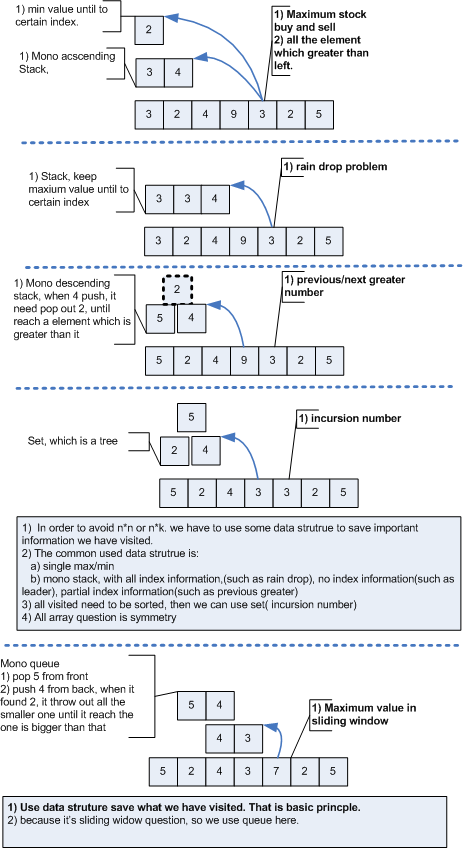
\includegraphics[scale=0.64]{pics/array.png} \newline
\end{center}
	
\section{Linked list}
\subsection{Basic}

	\par List in STL is bidirectional list(double-linked), in C++11, you can use \texttt{std::forward\_list} as single-linked list. 

\begin{lstlisting}[frame=single, language=c++]
struct node{   //C implementation
int a; 
 struct node* link
} ;

Template <class T> //C++ implementation
Class ChainNode{
   friend Chain<T>;
   T data
  ChainNode<T> *link;
}

template<class T>
class Chain{
	......
	ChainNode<T> *head;
}
\end{lstlisting}


\subsection{Operations}

\par Insert after p node, \textbf{get an index to previous pointer}
\begin{lstlisting}[frame=single, language=c++, mathescape=true]
//Consider if it's the first element. 
Insert(int k, const T &x)
chainNode<T> *i = new chainNode<T> (x);

//leftside is pointer pointed direction
//rightside is node, but in list, all nodes only can be accessed by a pointer.
//insert after p node 
i->link = p->link; //p->link is at right
p->link = i;       //p->link is at left now.
// i is inserted element, p is position.  
//You can remember i=p p=i  and fore three links.
\end{lstlisting}

	\par Insert before p node, what should I do?  \textbf{Just swap two node, then deal with next node. Don't touch next node in one atomic action. That is rule. }
\begin{lstlisting}[frame=single, language=c++, mathescape=true]
1)create temp auto node, new  i node.
 
while(p->link) 
2) copy value from p to temp node
3) copy value i to p.
4) copy temp value to i value
p = p->link.  
\end{lstlisting}

	\par Delete the node after a given node.
\begin{lstlisting}[frame=single, language=c++]
Delete(int k, const T&x)
d = p->link;
p->link = d->link ;
delete d;
//d=p p=d and last three links
\end{lstlisting}

	\par Delete the given node. That is a typical question. you need to remember it. 
\begin{lstlisting}[frame=single, language=c++]
void deleteNode(Node* node_ptr){
	// If the node to be deleted is the last node of linked list
	if (node_ptr->next == NULL){
		free(node_ptr); // this will simply make the node_ptr NULL.
		return;
	}
	
	// if node to be deleted is the first or any node in between the linked list.
	Node* temp = node_ptr->next;
	node_ptr->data = temp->data;
	node_ptr->next = temp->next;
	free(temp);
}
\end{lstlisting}
\begin{description}
	\item[Source code] Psychically, still delete the next node, logically, we use next value to overwrite current node value, so we simulate "delete" in this way. remember, \textbf{We don't need while loop to reach the last node in the list}. 
\end{description}

%	\item Indirect addressing combines array and list. You should store pointer in array, and each pointer refer to random storage object. A typical usage is char* [] each item in array is char*(string), when you sort the strings, you just move pointers. It will save a lot of move time.  

	\par Three different operations:
\begin{itemize}
	\item Normal single link list: insert and delete given a node, always insert after the given node, or erase the next node of the given node. 
	
	\item Normal single link list: If you want to insert before or delete the given node, You still need to do it physically, but copy value to simulate the "insert" and "delete". 
	
	\item Double link list, such as \texttt{std::list}, insert value before the given node, and delete the given node. 
\end{itemize}


	\par How to rotate a List? This question in interesting, you need to understand splice usage. splice perform 1) move like question, 2) before node of next(i,3) points to null, 3) pointer of end(li) points to i. All these things perform automatically. 

\begin{lstlisting}[frame=single, language=c++]
list<int> li = {1, 2, 3, 4, 5};
auto i = begin(li);
//rotate(i, std::next(i, 3), end(li) ); //must use std::next complexity is O(n).
li.splice(i, li, next(i, 3), end(li) ); //better, use splice, O(1)
\end{lstlisting}



\subsection{Interview questions}
\begin{itemize}
	\item Use dumb head for easy deleting node. 
\begin{lstlisting}
while (head != NULL && head->val == val) { // pay attention while here, 
	ListNode* tmp = head;     //5-->5-->5--> for this condition.
	head = head->next;
	delete tmp;
}

// delete non head 
ListNode* cur = head;
while (cur != NULL && cur->next!= NULL) {
	if (cur->next->val == val) {
		ListNode* tmp = cur->next;
		cur->next = cur->next->next;
		delete tmp;
	} else {
		cur = cur->next;
	}
}
return head;
}
\end{lstlisting}

	If we build dumb node, code is much easier now
\begin{lstlisting}
ListNode* dummyHead = new ListNode(0); // dumb node
dummyHead->next = head; 
// Set the virtual (dummy) head node to point to the head, which makes it easier to perform deletion operations later.
ListNode* cur = dummyHead;

while (cur->next != NULL) {
	if(cur->next->val == val) {
		ListNode* tmp = cur->next;
		cur->next = cur->next->next;
		delete tmp;
	} else {
		cur = cur->next;
	}
}
return dummyHead->next;
\end{lstlisting}
	
	\item Print the middle element of link list. When exit while, even node, fast\_ptr will be NULL, odd node, fast\_ptr->next will be null. Just like n/2, odd number will be in the middle, even number will be the first element in the second half.
\begin{lstlisting}[breaklines]
void printMiddle(struct Node *head) { 
	struct Node *slow_ptr = head; 
	struct Node *fast_ptr = head; 

	if (head!=NULL) {		 
		while (fast_ptr != NULL && fast_ptr->next != NULL) {  //this statement is very important.
			fast_ptr = fast_ptr->next->next; 
			slow_ptr = slow_ptr->next; 
		} 
		printf("The middle element is [%d]\n\n", slow_ptr->data); 
	} 
} 
\end{lstlisting}
	
	\item How to reverse a list \textbf{ There are two points: 1)while(p),  2) inside loop, do p = p->next, and necessary action( print out value and change pointer direction...)}

\begin{center}
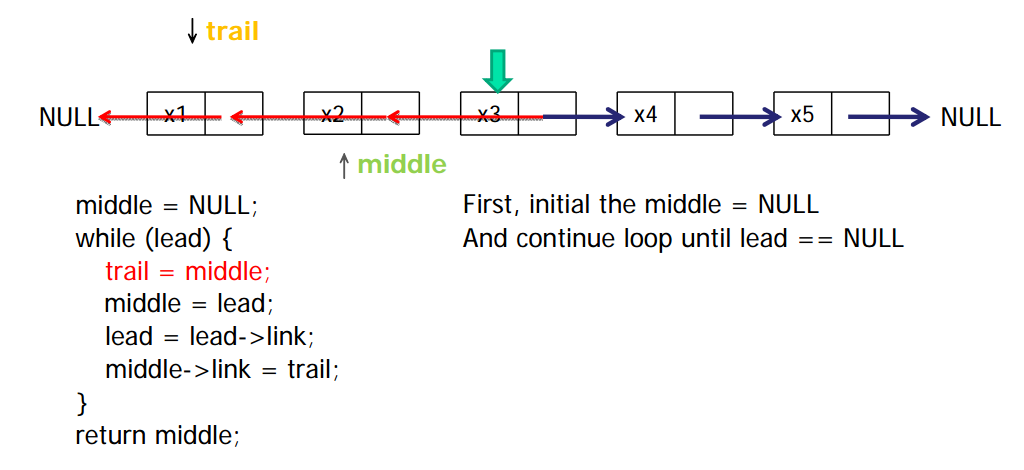
\includegraphics[scale=0.65]{pics/reverse.png} 
\end{center}

\begin{lstlisting}[breaklines]
node* lead, middle, *tail;
middle = nullptr;
tail = head;
while(tail){
	lead = middle;
	middle = tail;
	tail = tail->next;
	middle->next = lead;
}
head = middle;
\end{lstlisting}

%\begin{description}
%	\item[line] end condition
%	\item[line] end-input condition
%	\item[line] begin condition
%	\item[line] begin-input condition
%\end{description}

%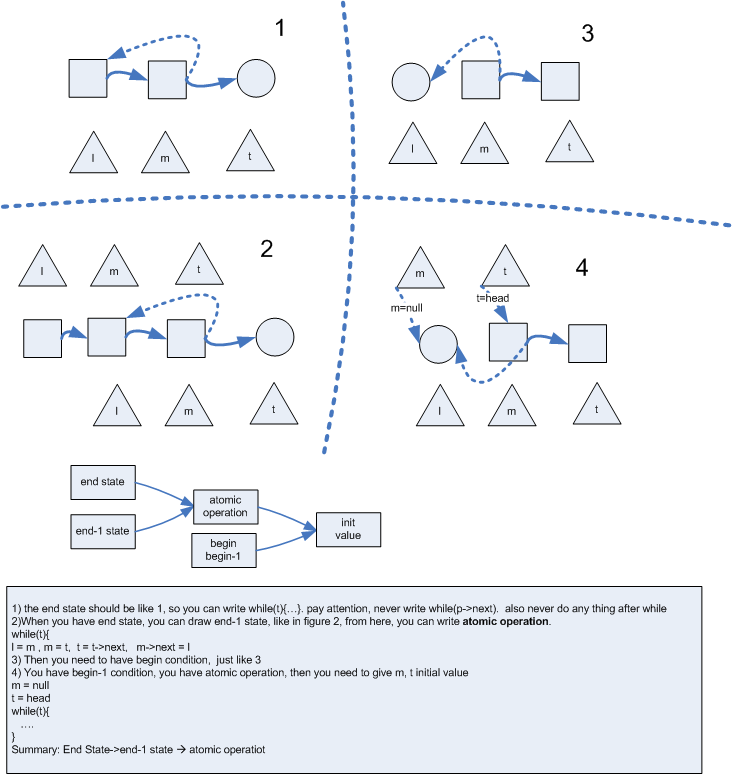
\includegraphics[scale=0.60]{pics/link.png} \newline
%
\item Three steps to resolve this problem. this pattern can be applied on all link list problem. 
\begin{enumerate}
	\item The end status is like below figure.
	
	\item so normal status is also like this(previous atomic operation end statu and next atomic operation start status are all like below ), write while main logic.
	
	\item when you finish while main logic, according to this logic customize your beginning status. in this question, only tail = head and middle = nullptr;
\end{enumerate}

\begin{center}
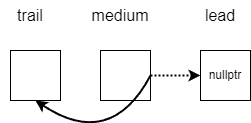
\includegraphics[scale=0.48]{pics/reverse_list.drawio.png}
\end{center}

	\item Reverse linklist 
\begin{lstlisting}
// Definition: Given the head node of a singly linked list, reverse the list and return the new head node.
ListNode reverse(ListNode head) {
	if (head == null || head.next == null) {
		return head;
	}
	ListNode last = reverse(head.next);
	head.next.next = head;
	head.next = null;
	return last;
}
//1) in reverse, we don't use last node 
//2) in each reverse, we just take action, don't need return something. 
//3) just like reverse output a linklist.


//below is my implementation, Pay attention to the ListNode* &, we need to modify 
//head->next, so we have to return reference. just return pointer doesn't work here. 
ListNode* ghead;
ListNode * &  dfs(ListNode* head){
	if(head == nullptr){
		ghead = head;
		return ghead;
	}
	if(head->next == nullptr){
		ghead = head;
		return ghead->next;
	}
	ListNode* & p = dfs(head->next);
	cout<<head->val<<endl;
	p=head;
	head->next = nullptr;
	return head->next;
}

ListNode* reverseList(ListNode* head) {
	dfs(head);
	return ghead;      
}
\end{lstlisting}

\begin{center}
	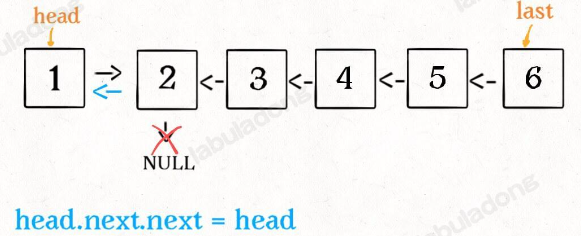
\includegraphics[scale=0.46]{pics/re.png}
\end{center}

\item Reverse the first k element
\begin{lstlisting}
ListNode successor = null; // Successor node
// Reverse the first n nodes starting from head and return the new head node
ListNode reverseN(ListNode head, int n) {
	if (n == 1) { // Record the (n + 1)th node
		successor = head.next;
		return head;
	}
	// Starting from head.next, reverse the first n - 1 nodes
	ListNode last = reverseN(head.next, n - 1);
	
	head.next.next = head;
	// Connect the reversed head node to the successor node
	head.next = successor;
	return last;
}
\end{lstlisting}

\item Reverse m to n 
\begin{lstlisting}
ListNode reverseBetween(ListNode head, int m, int n) {
	// base case
	if (m == 1) {
		return reverseN(head, n);
	}
	
	// advance to revert beginning point to trigger base case.
	head.next = reverseBetween(head.next, m - 1, n - 1);
	return head;
}
\end{lstlisting}


\item Per k group to reverse 
\begin{lstlisting}
/** Reverse elements in the interval [a, b), note that it's left-closed and right-open */
ListNode reverse(ListNode a, ListNode b) {
	ListNode pre = null, cur = a, nxt = a;
	// Just change the while loop's termination condition
	while (cur != b) {
		nxt = cur.next;
		cur.next = pre;
		pre = cur;
		cur = nxt;
	}
	// Return the new head node after reversal
	return pre;
}

ListNode reverseKGroup(ListNode head, int k) {
	if (head == null) return null;
	// Interval [a, b) contains k elements to be reversed
	ListNode a = head, b = head;
	for (int i = 0; i < k; i++) {
		// If fewer than k nodes, no need to reverse; base case
		if (b == null) return head;
		b = b.next;
	}
	// Reverse the first k elements
	ListNode newHead = reverse(a, b);
	// Recursively reverse the remaining list and connect them
	a.next = reverseKGroup(b, k);
	return newHead;
}
\end{lstlisting}

	\item Given a singly linked list, determine if its a palindrome. This method takes O(n) time and O(1) extra space.
\begin{enumerate}
	\item Get the middle of the linked list.
	\item Reverse the second half of the linked list.
	\item Check if the first half and second half are identical.
	\item \textbf{Idea: 1) find the middle 2)reverse}. If it's odd number,  you need to move the middle pointer to next position.
\end{enumerate}


	\item Swap nodes in a linked list without swapping data. The idea it to first search x and y in given linked list. If any of them is not present, then return. While searching for x and y, keep track of current and previous pointers.
\begin{lstlisting}[frame=single, language=c++] 
/* Split the nodes of the given list into front and back halves,
     and return the two lists using the reference parameters.
     If the length is odd, the extra node should go in the front list.
     Uses the fast/slow pointer strategy.  */
void FrontBackSplit(struct node* source,
          struct node** frontRef, struct node** backRef)
{
  struct node* fast;
  struct node* slow;
  if (source==NULL || source->next==NULL){
    /* length < 2 cases */
    *frontRef = source;
    *backRef = NULL;
  }
  else{
    slow = source;
    fast = source->next;
 
    /* Advance 'fast' two nodes, and advance 'slow' one node */
    while (fast != NULL){
      fast = fast->next;
      if (fast != NULL){
        slow = slow->next;
        fast = fast->next;
      }
    }
 
  /*'slow' is before the midpoint in the list, so split it in two at that point.*/
    *frontRef = source;
    *backRef = slow->next;
    slow->next = NULL;
  }
}

\end{lstlisting}


	\item Prints the given Linked List in reverse manner. (resurisve)
\begin{lstlisting}[frame=single, language=c++]
void fun1(struct node* head){
  if(head == NULL)
    return;
  
  fun1(head->next);
  printf("%d  ", head->data);
}
\end{lstlisting}

	\item Write a program function to detect loop in a linked list
\begin{lstlisting}[breaklines]
This is the fastest method. Traverse linked list using two pointers.  Move one pointer by one and other pointer by two.  If these pointers meet at some node then there is a loop.  If pointers do not meet then linked list doesn't have loop.
\end{lstlisting}
\textbf{a circle has at last three nodes, so fast pointer each time step 2, So it will always go around inside the circle}

	\par Summary of link list:
\begin{itemize}
\item \textbf{Just like tree, most link-list problems can be resolved by recursive}.

\item Most of time, In single link list, you need to keep previous node and current node. 
\end{itemize}

\begin{tabular}{|c|c|c|}
\hline 
 & array & list \\ 
\hline 
insert erase & O(n) & O(1) \\ 
\hline 
sort & quicksort & mergesort  \\ 
\hline 
reverse & swap element & just manipulate pointer  \\ 
\hline 
rotate & easy pointer manipulate & swap element  \\ 
\hline 
merge &  &  \\ 
\hline 
other  &  &  \\ 
\hline 
\end{tabular} 


\par \texttt{std::list} has its own sort member function, but \texttt{std::vector} doesn't have. you can use std::sort algorithme. \texttt{std::list} has its own reverse,  std::vector doesn't have, just use std::reverse algorithm. std::list and vector don't have their own rotate function. \texttt{std::list} has its own merge, vector use std::merge algorithm.

\end{itemize}


\section{Matrix}
\subsection{Sparse matrices}

	\par Sparse matrix can implemented by on dimension array or linked list. 
\begin{lstlisting}[frame=single, language=c++]
template<typename T>
class term{
	int row, int col;
	T value;
}

term<T> *sparseMatrix;	// using one linked list
\end{lstlisting}

	\par Define sparse matrix by using std::list. 
\begin{lstlisting}
using Row = list< pair<int, float> > ;
using Matrix = list< int, Row>;

list< pair<int, float> > row0;
row0.push_back({0, 1.0});
row0.push_back({3, 3.0});

Matrix matrix;
matrix.push_back({0, row0});
\end{lstlisting}


%\begin{lstlisting}[frame=single, language=c++]
%	template<typenameT>
%	class CNode{
%		int col;
%		T value;
%	};
%	
%	
%	
%	template<typename T>
%	class HeadNode{
%		int row, 
%		Chain< CNode<T> > colFirst
%	};
%	
%	template<typename T>
%	class Matrix{
%		Chain< HeadNode<T> > Frist
%	} 
%\end{lstlisting}


	\par You can build a matrix class. use m(2,3) to access a element. And support +, - * . You also can define index begin from 1. It will more reasonable for you when you use a matrix. 
\begin{lstlisting}[frame=single, language=c++]
template<typename T>
class Matrix{
	T& operator()(int row, int col){
		..
	}
}	
\end{lstlisting} 


\par  Some special square matrices
\begin{itemize}
	\item Diagonal  $i\neq j, M(i,j) = 0$ Can use one dimension array to describe it. 
	
	\item Low triangular $i<j, M(i,j) = 0$ We can use one dimension array to implement lower triangular because it will save many spaces.  Index can be calculated by $i*(i-1)/2+j-1$, and save it into a one dimension array. 

\begin{lstlisting}
[a11  0   0   0 ]
[a21 a22  0   0 ]
[a31 a32 a33  0 ]
[a41 a42 a43 a44]

a11: (1 - 1) * (1) / 2 + 1 - 1 = 0
a21: (2 - 1) * (2) / 2 + 1 - 1 = 1
a22: (2 - 1) * (2) / 2 + 2 - 1 = 2
a31: (3 - 1) * (3) / 2 + 1 - 1 = 3
a32: (3 - 1) * (3) / 2 + 2 - 1 = 4
.....
\end{lstlisting}
	
	\item Symmetric. Just like a low triangular matrix, can be described by one dimension array. 
\end{itemize}

\subsection{Matrices traversal methods and operation}
	
\begin{itemize}
	
	\item Row and column traversal, just use two for statement. Pay attention to the cache missing problem when you perform column traversal. 
	
	\item For square matrix (n*n), you can perform in place transpose. There are two points:
\begin{enumerate}
	\item Swap \texttt{i} and \texttt{j}. 
	\item If botton-left to top-right, then use \texttt{n-1} to substract.
\end{enumerate}
\begin{lstlisting}
 for (int i = 0; i < n; i++) {
	for (int j = i; j < n; j++) {
		 swap(matrix[i][j], matrix[j][i]);
	}
}

// Mirror-symmetric 2D matrix along the bottom-left to top-right diagonal.
for (int i = 0; i < n; i++) {
	for (int j = 0; j < n - i; j++) {
		 swap(matrix[i][j], matrix[n-1-j][n-1-i]);
	}
}
\end{lstlisting}

	\item Rotate clockwise or counter clockwise matrix, first transpose, then reverse each row, just remember this trick. 
	
	\item Spiral print a matrix. Four boundary, then shrink step by step. 
\begin{lstlisting}
int m = matrix.length, n = matrix[0].length;
int upper_bound = 0, lower_bound = m - 1;
int left_bound = 0, right_bound = n - 1;
List<Integer> res = new LinkedList<>();
// When res.size() == m * n, the entire array has been traversed
while (res.size() < m * n) {
	if (upper_bound <= lower_bound) {
		// Traverse from left to right on the top
		for (int j = left_bound; j <= right_bound; j++) {
			res.add(matrix[upper_bound][j]);
		}
		upper_bound++; // Move the upper boundary down
	}
	
	if (left_bound <= right_bound) {
		// Traverse from top to bottom on the right side
		for (int i = upper_bound; i <= lower_bound; i++) {
			res.add(matrix[i][right_bound]);
		}
		right_bound--; // Move the right boundary left
	}
	
	if (upper_bound <= lower_bound) {
		// Traverse from right to left on the bottom
		for (int j = right_bound; j >= left_bound; j--) {
			res.add(matrix[lower_bound][j]);
		}
		lower_bound--; // Move the lower boundary up
	}
	
	if (left_bound <= right_bound) {
		// Traverse from bottom to top on the left side
		for (int i = lower_bound; i >= upper_bound; i--) {
			res.add(matrix[i][left_bound]);
		}
		left_bound++;  // Move the left boundary right
	}
}
\end{lstlisting}

	\item DFS, recursive and iterator implementation.
\begin{lstlisting}
//leetcode 200, Main function to count the number of islands
int numIslands(char[][] grid) {
	int res = 0;
	int m = grid.length, n = grid[0].length;
	for (int i = 0; i < m; i++) { // Traverse the whole grid
		for (int j = 0; j < n; j++) {
			if (grid[i][j] == '1') {
				// Increase the island count when a new island is found.
				res++;
				dfs(grid, i, j); // Then use DFS to sink the island.
			}
		}
	}
	return res;
}

// Starting from (i, j), turn all adjacent land into water
void dfs(char[][] grid, int i, int j) {
	int m = grid.length, n = grid[0].length;
	if (i < 0 || j < 0 || i >= m || j >= n) {
		return; // Out of index bounds
	}
	if (grid[i][j] == '0') {
		return; // Already water
	}
	
	grid[i][j] = '0'; // Turn (i, j) into water
	// Sink the land above, below, left, and right
	dfs(grid, i + 1, j);
	dfs(grid, i, j + 1);
	dfs(grid, i - 1, j);
	dfs(grid, i, j - 1);
}	
\end{lstlisting}

	\par There are a few points you need to pay attention to when you implement dfs by iteration:
	
\begin{enumerate}
	\item top and pop should stay together; 
	\item use pair to remember position, 
	\item use s!=empty(); 
	\item check four boundary,  
	\item when pop, check if we visited, when push, check if we visited. (two positions checks) 
\end{enumerate}

\begin{lstlisting}
void dfs(vector<vector<char>>& grid, int i, int j){
	int row = grid.size();
	int col = grid[0].size();
	if(grid[i][j] == '0'){
		return ;
	}
	
	stack<pair<int, int> > s;
	s.push({i,j});
	while(!s.empty()){
		auto [i,j] = s.top(); //top and pop should be stay together 
		s.pop();              
		if(grid[i][j] == '1'){
			grid[i][j] = '0';
			if(i>0 && grid[i-1][j] == '1'){
				s.push({i-1, j});
			}
			if(j<col-1 && grid[i][j+1] == '1'){
				s.push({i, j+1});
			}
			if(i<row-1 && grid[i+1][j] == '1'){
				s.push({i+1, j});
			}
			if(j>0 && grid[i][j-1] == '1'){
				s.push({i, j-1});
			}
		}	
	} 
}	
\end{lstlisting}


	\item BFS. A few difference with DFS:
\begin{enumerate}
	\item No need to check when pop, because when we push, we have visited, all the node in queue are visited. 
	
	\item Change stack to queue, change top to front.
	
	\item When add the first element, mark it as visited.  
\end{enumerate}
	 
\begin{lstlisting}
 void BFS(vector<vector<char>>& grid, int i, int j){
	int row = grid.size();
	int col = grid[0].size();
	if(grid[i][j] == '0'){
		return ;
	}
	
	queue<pair<int, int> > q;
	q.push({i,j});
	grid[i][i] = '0'; //the first element also need to marked as visited. 
	while(!q.empty()){
		auto [i,j] = q.front();
		q.pop();
		cout<<i<<" "<<j<<endl;
		if(i>0 && grid[i-1][j] == '1'){
			grid[i-1][j] = '0';
			q.push({i-1, j});
		}
		if(j<col-1 && grid[i][j+1] == '1'){
			grid[i][j+1] = '0';
			q.push({i, j+1});
		}
		if(i<row-1 && grid[i+1][j] == '1'){
			grid[i+1][j] = '0';
			q.push({i+1, j});
		}
		if(j>0 && grid[i][j-1] == '1'){
			grid[i][j-1] = '0';
			q.push({i, j-1});
		}      
	}
}
\end{lstlisting}

\begin{center}
	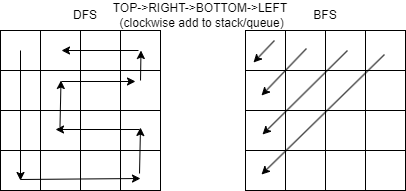
\includegraphics[scale=0.70]{pics/dfs_bfs.drawio.png}
\end{center}

\end{itemize}	

\par About the traversing direction 
\begin{itemize}

	\item  Reverse traverse, from bottom to up, from left to right.
\begin{lstlisting}
for (int i = n - 1; i >= 0; i--) {
	for (int j = i + 1; j < n; j++) {
		dp[i][j] = max(dp[i + 1][j], dp[i][j - 1]);	 // current after left and right cell
\end{lstlisting}

\begin{center}
	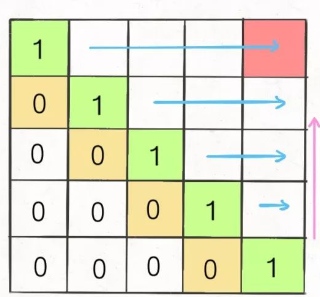
\includegraphics[scale=0.40]{pics/mr.png}
\end{center}

	\item Diagonal traverse
\begin{lstlisting}
for (int l = 2; l <= n; l++) { //l is length.
	for (int i = 0; i <= n - l; i++) {
		int j = l + i - 1;
		// dp[i][j]
	}
}
      i:= 0..........n
l:=2  (0,1) (1,2) (2,3)
l:=3  (0,2) (1,3) (2,4)
l:=4  .......
\end{lstlisting}
		
\begin{center}
	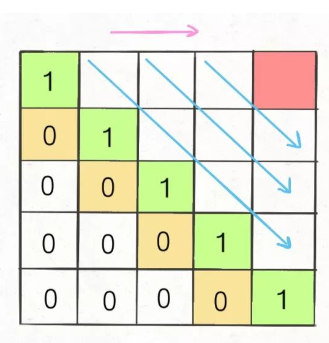
\includegraphics[scale=0.40]{pics/md.png}
\end{center}		
	 
	
	
	\item The most implicated traversal, dp to calculate matrix multiplication. How to a kind of diagonal traversal matrix? this method is useful for matrix multiplication DP problem. 
	
\begin{lstlisting}
for(L = 2;L<n;L++)
  for(i = 1;i<n-L+1;++i)  //n-L+1  remember n-L+1 and i+L-1. 
     j = i+L-1            //i+L-1
  	for (k = i; k <= j - 1; k++){
  		...
\end{lstlisting}

\begin{center}
	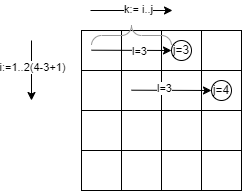
\includegraphics[scale=0.60]{pics/transversal.drawio.png} 
\end{center}
	

\end{itemize}

	\par Fill and color difference. if you want to color fill, need to check if origin color and new color are the same, otherwise, it will lead dead loop. 
	

%	\par  You can use two dimensions array to act as a matrix, square matrix, diagonal matrix, lower triangular, symmetric. 
	
	\par \textbf{matrix and spiral print all indicate a good hint:} 
	
	\begin{itemize}
		\item identify a sub task(function).
		
		\item then design this function API (what information this function need to finish it's task.) 
		
		\item Once we have correct API, then loop call this function with correct parameter, this step will be easy now. 
	\end{itemize}
	
\subsection{Interview questions}
\begin{itemize}
	
	\item leetcode 48. You are given an n x n 2D matrix representing an image, rotate the image by 90 degrees (clockwise). You have to rotate the image in-place, which means you have to modify the input 2D matrix directly. DO NOT allocate another 2D matrix and do the rotation.
	
	\item Two matrix multiply. \texttt{sum += v1[row][i]*v2[i][col];} is the key points to understand the whole problem. 
\begin{lstlisting}[]
int inner_product(int row, int col, int num, const vector<vector<int>> &v1, 
const vector<vector<int>> &v2){
	int sum = 0;
	for (int i =0 ;i<num ;i++){
		sum += v1[row][i]*v2[i][col];
	}
	return sum;
}
vector<vector<int> > m1 = {{1,2,3}, {4, 5, 6}}; //list initialization
vector<vector<int> >m2 = { {1,2}, {3,4}, {5,6}};

int m1_row = m1.size(); int m1_col = m1[0].size();
int m2_row = m2.size(); int m2_col = m2[0].size();
vector<vector<int> > result = {{0,0}, {0,0}};
for(int i = 0;i<m1_row;i++){
	for(int j= 0;j<m2_col;j++){
		int element = inner_product(i, j,3, m1, m2); //call function here.
		result[i][j] = element;
	}
}		
\end{lstlisting}
	
	\begin{description}	
		\item[Source code] In this questions, inner\_product is key point to resolve this problem. First, get atomic operation and change it into a function. Then, design this function parameter and in the end, design outside environment to call this automic function. This is very an important strategy. 
	\end{description}
	
	
%	\item Spiral print a matrix
%	\begin{lstlisting}[numbers=none]
%		int
%		print_out (int rb, int re, int cb, int ce, bool isrow, bool positive,
%		const vector < vector < int >>&v)
%		{
%			if (isrow){
%				if (positive){
%					for (int i = cb; i <= ce; i++){
%						cout << v[rb][i]<<',';
%					}
%				}
%				else{
%					for (int i = ce; i >= cb; i--){
%						cout << v[re][i]<<',';
%					}
%				}
%			}
%			else
%			{
%				if (positive){
%					for (int i = rb; i <= re; i++){
%						cout << v[i][ce]<<',';
%					}
%				}
%				else{
%					for (int i = re; i >= rb; i--){
%						cout << v[i][cb]<<',';
%					}
%				}
%			}
%		}
%		
%		int main ()
%		{
%			vector < vector < int >>m1 = { {1, 2, 3}, {4, 5, 6}, {7, 8, 9} };
%			int row = m1.size()-1;
%			int col = m1[0].size()-1;
%			
%			int rb = 0, re = row, cb = 0, ce = col;
%			int isrow = 1;
%			int positive = 1;
%			while (rb <= re && cb <= ce){
%				
%				if (isrow == 1 && positive == 1)
%				{
%					print_out (rb, re, cb, ce, isrow, positive,m1);
%					rb++;
%					isrow = 0;
%					positive =1;
%				}
%				if (isrow == 0 && positive == 1)
%				{
%					print_out (rb, re, cb, ce, isrow, positive,m1);
%					ce--;
%					isrow = 1;
%					positive = 0;
%				}
%				if (isrow == 1 && positive == 0)
%				{
%					print_out (rb, re, cb, ce, isrow, positive,m1);
%					re--;
%					isrow = 0;
%					positive = 0;
%				}
%				if (isrow == 0 && positive == 0)
%				{
%					print_out (rb, re, cb, ce, isrow, positive,m1);
%					cb++;
%					isrow = 1;
%					positive = 1;
%				}
%			}
%			return 0;
%		}	
%		
%	\end{lstlisting}		
%	
%	\begin{description}
%		\item[line ] \textbf{In this questions, print\_out is key. }
%		\item[line ] \textbf{Get atomic operation, print\_out, design the interface of this key function. after it, design the context which use this key function: print\_out. In this context, usually involve a loop and change boundary parameter.}
%		
%		\item[line ] rb, re, cb, ce very good clue, once you found these four parameters, then this question becomes easier. another two useful flag is isrow and positive. 
%	\end{description}
	
	
	
\end{itemize}

 
\section{Stack}

	\par In C++ STL , \texttt{std::stack} is container adaptor, specifically designed to operate in a LIFO context. Stack is last-in first-out, and queue is frist-in and first-out


\subsection{Application of Stack}

		
\par The most famous application about stack is \textbf{Recursive}. \textbf{The most famous applications based on stack is:  Maze (depth first search). Hanoi tower (Recursive). brace Match.}  



	\par Some typical two stacks examples. One is expressions evaluation. we can build two stacks, one is for operands and the other for operators. When the operators precedence is higher than the stack top element, push the operators into the stack, otherwise, pop the operator and get two operatands from operands stacks, get the result and push back to the operands stack.  
	\begin{center}
			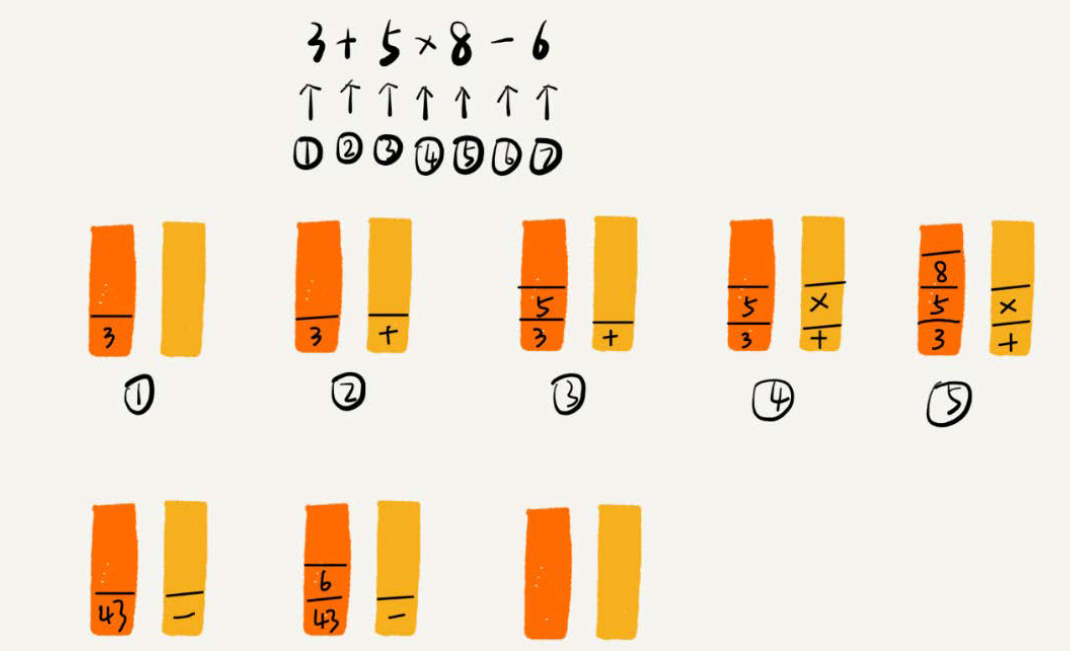
\includegraphics[scale=0.4]{pics/stacks_two.png} 
	\end{center}

	\par Two stacks trick can also be used in browsers back and forward function. Another typical two stack usage are use two stacks to implement queue.

\begin{minipage}{.5\textwidth}		
	\begin{center}
		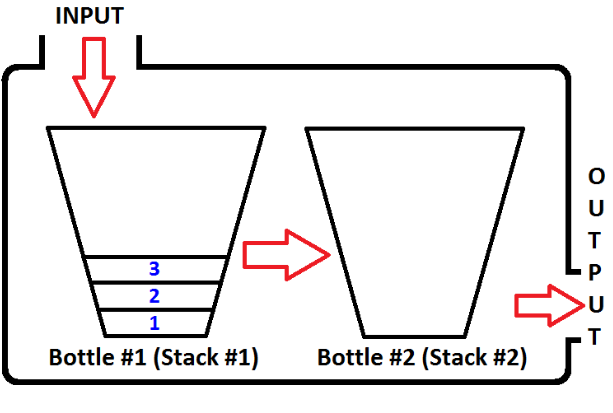
\includegraphics[scale=0.25]{pics/sq1.png} 
	\end{center}
\end{minipage}	
\begin{minipage}{.5\textwidth}		
	\begin{center}
		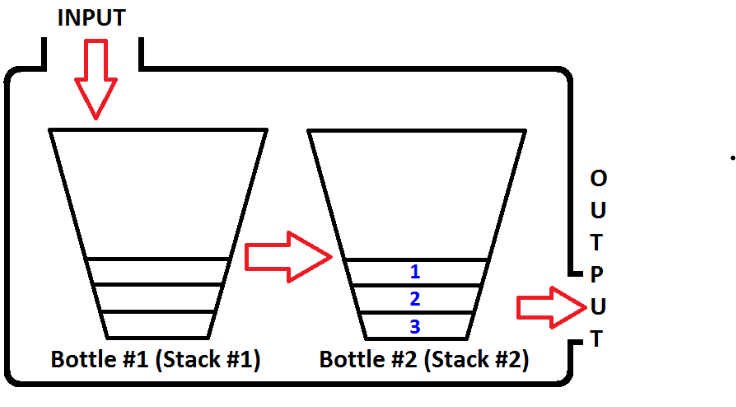
\includegraphics[scale=0.25]{pics/sq2.png} 
	\end{center}
\end{minipage}

\subsubsection{Offline Equivalence class}

	\par Offline equivalence class, known n and R, get all Equivalence class. 
	
	\par n = 9, r = 11 and relation pairs are:
	(1,5), (1,6),(3,7),(1,5), (4,8),(5,2)
	(6,5), (4,9),(9,7),(7,8), (3,4),(6,2)
	
	
	
	\par One word, \textbf{from relation pairs build a graphs(adjacency list), Then use stack to perform DFS search, use equivalence class record if we have visited.}
	
	
	
	Phase 1: Equivalence pairs (i, j) are read in and adjacency (linked) list of each object is built. Phase 2: Trace (output) the equivalence class containing object i with stack (depth-first search). Next find another object not yet output, and repeat.
	
\begin{lstlisting}[frame=single, language=c++, basicstyle=\scriptsize]
for (int i = 1; i <= n; i++)  // output equivalence classes
if  (!out[i]) { // start of a new class
	out[i] = true;
	unprocessedList.push(new Integer(i)) ;
	while (!unprocessedList.empty()) { 
		// get rest of class from unprocessedList
		int j = ((Integer) unprocessedList.pop()).intValue();
		while  (!list[j].empty()) { 
			// elements on list[j] are in the same class
			int q = ((Integer) list[j].pop()).intValue();
			if (!out[q]) { // q not yet output
				System.out.print(q + " ");
				out[q] = true;
				unprocessedList.push(new Integer(q));  }
		} //end of while
	}  //end of while 
} //end of if	
\end{lstlisting}	
	
\begin{minipage}{.5\textwidth}	
		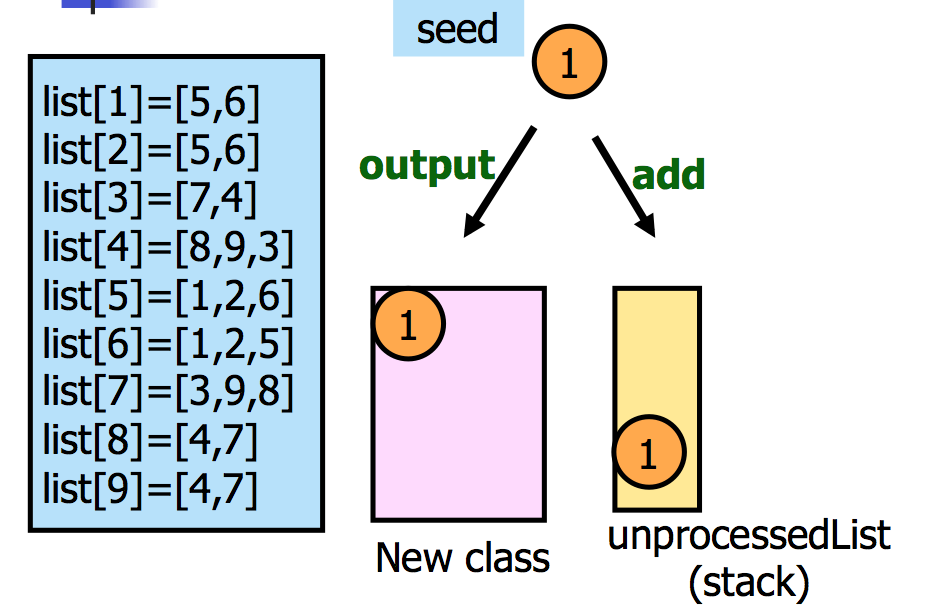
\includegraphics[scale=0.35]{pics/offline_1.png} 
\end{minipage}
\begin{minipage}{.5\textwidth}	
	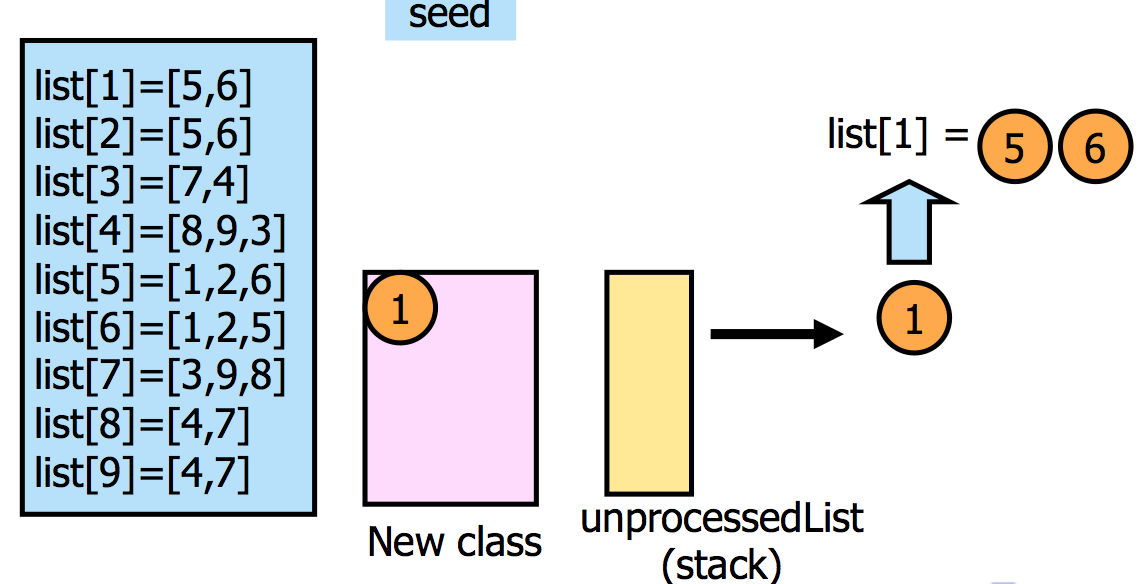
\includegraphics[scale=0.35]{pics/offline_2.png}  
\end{minipage}

\begin{minipage}{.5\textwidth}	
	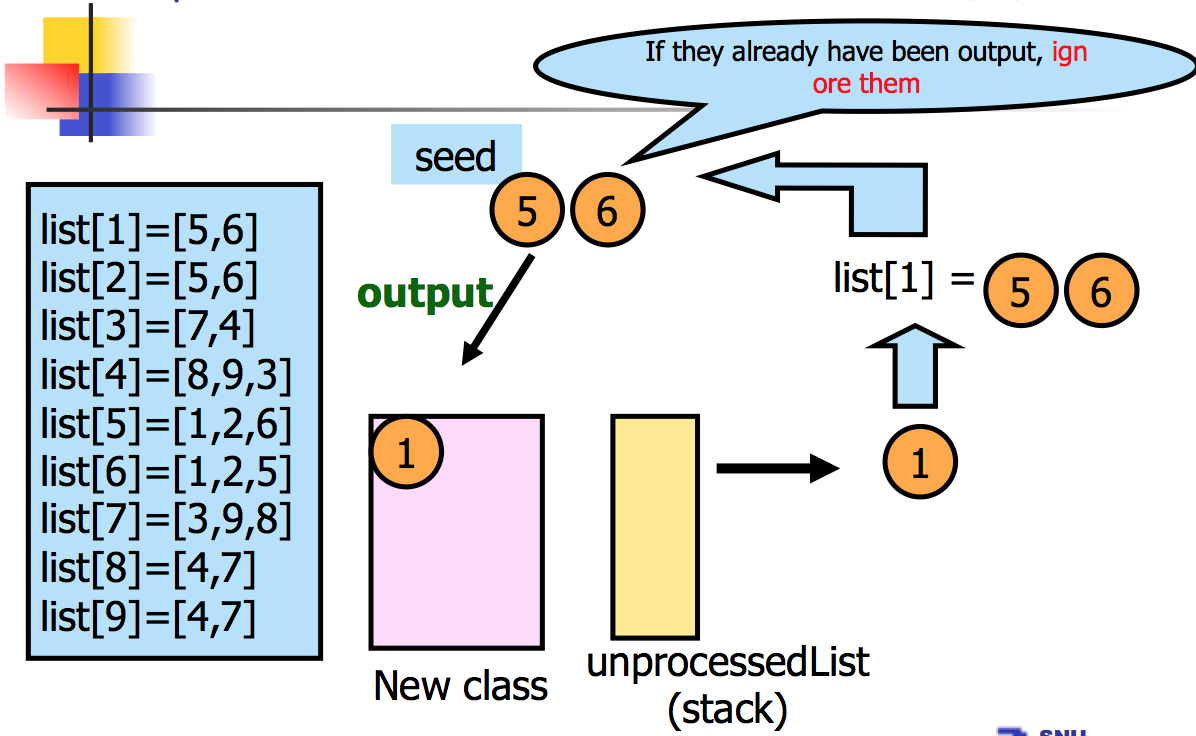
\includegraphics[scale=0.35]{pics/offline_3.png} 
\end{minipage}
\begin{minipage}{.5\textwidth}	
	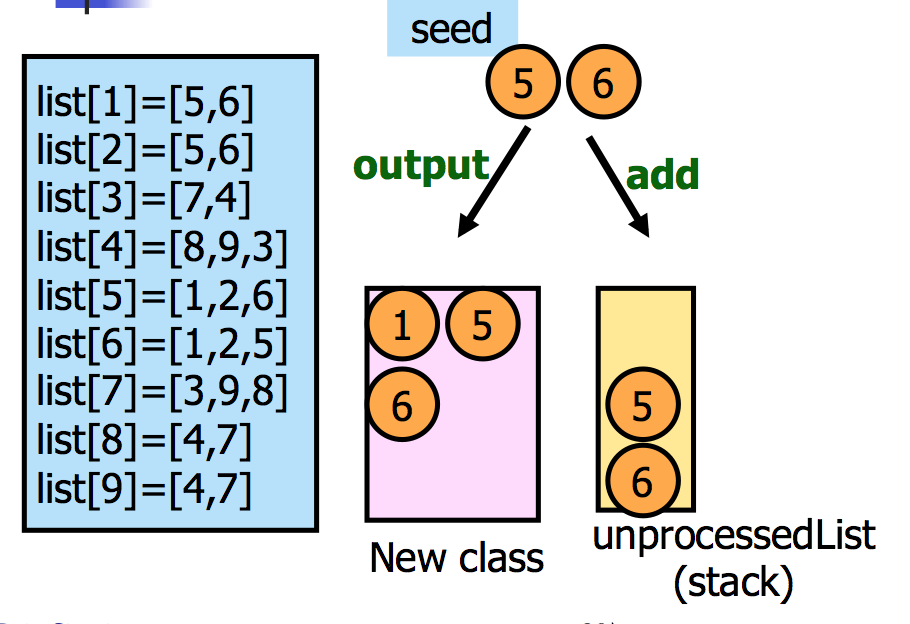
\includegraphics[scale=0.35]{pics/offline_4.png}  
\end{minipage}

\begin{minipage}{.5\textwidth}	
	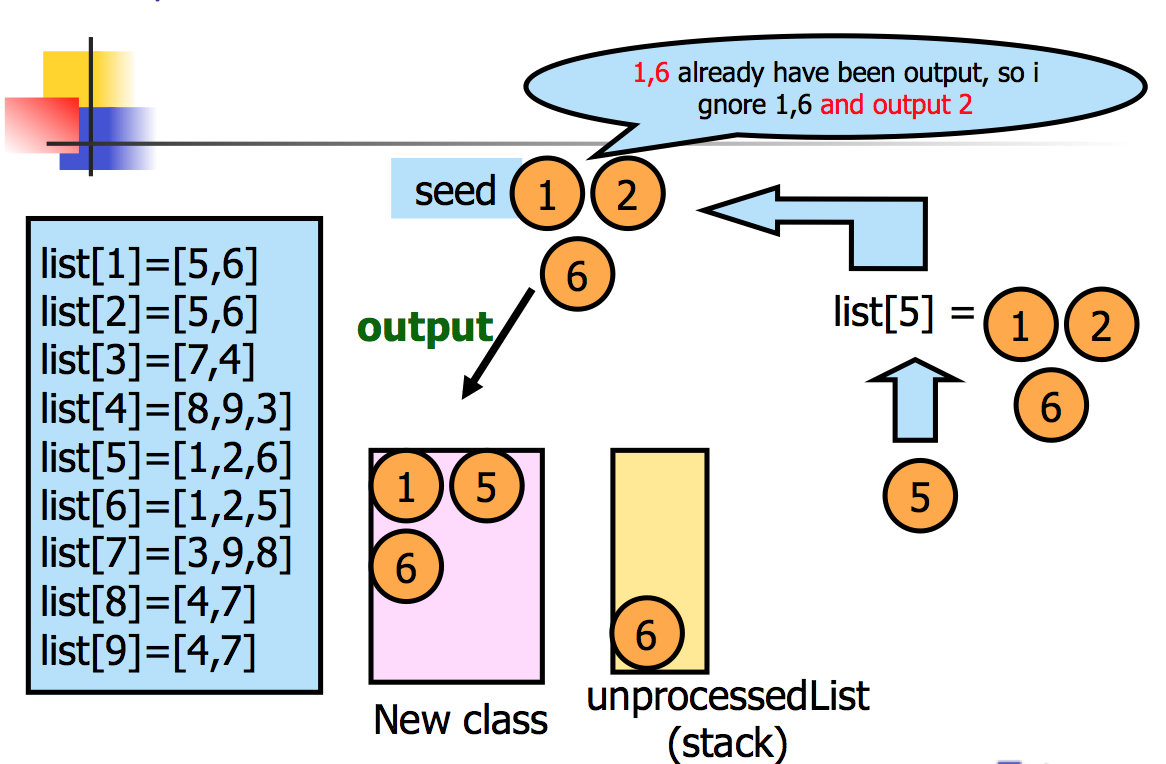
\includegraphics[scale=0.35]{pics/offline_5.png} 
\end{minipage}
\begin{minipage}{.5\textwidth}	
	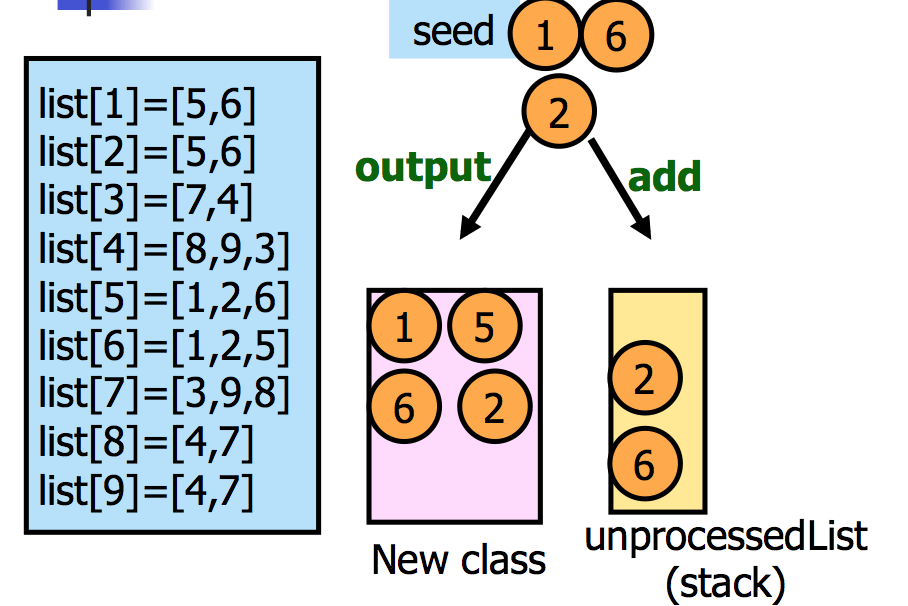
\includegraphics[scale=0.35]{pics/offline_6.png}  
\end{minipage}


\subsection{Interview questions}
\begin{itemize}

\item MinStack, all operation are constant time. Design a Data Structure SpecialStack that supports all the stack operations like push(), pop(), isEmpty(), isFull() and an additional operation getMin() which should return minimum element from the SpecialStack. All these operations of SpecialStack must have a time and space complexity of O(1). 
Note: To implement SpecialStack, you should only use standard Stack data structure and no other data structure like arrays, lists, etc 
\begin{lstlisting}[frame=single, language=c++, basicstyle=\scriptsize]
class MinStack {
public:
	void push(int val) {
		if (stack.empty()) {
			stack.push_back({val, val});
		} else {
			stack.push_back({val, min(stack.back().second, val)});
		}
	}
	void pop() {
		stack.pop_back();
	}
	int top() {
		return stack.back().first;
	}	
	int getMin() {
		return stack.back().second;
	}
private:
	// first = val, second = min as of that insert
	vector<pair<int, int> > stack;
};	
\end{lstlisting}

\end{itemize}

\section{Queue}

\subsection{Circule Queue}

	
\par You can use three different way to implement queue, array, linked list and circular array.
	
\par Circular array representation of a queue. 

\begin{center}
	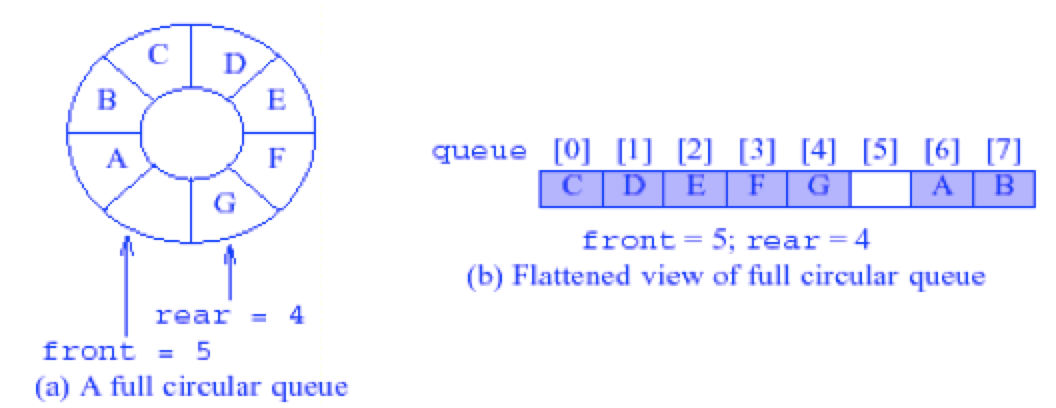
\includegraphics[scale=0.35]{pics/cd.png} 
\end{center}

\begin{itemize}
\item Initial condition : front = rear = 0

\item front is for pop, rear is for push (STL use back), so you can remember it easily.

\item use rear+1\%length and front+1\%length to simulate rear++ and front++

\item rear+1\%length == front means full;  front==rear is empty.

\item \textbf{front point to an empty cell. So at most it can save length-1 elements. } Otherwise, we can't distinguish empty and full.


\item how to understand (rear+1)\%length. an array with 10 element, length is 10, the last index is 9.  (9+1)\%10 = 0, it help use change 9 to 0(from end array to begin array)

\begin{lstlisting}[frame=single, language=c++]
void push(T t){
	if ((rear+1)%length == front){
		throw "full" exception
	}
	rear = (rear+1)%length; //use (rear+1)%length simulate ++rear
	array[rear] = t;
}	
\end{lstlisting}

\item Pop only increase front, so if front == rear, means front catch up rear, it means empty.
\begin{lstlisting}[frame=single, language=c++]
T pop(){
	if (front == rear){
		throw "empty" exption
	}
	front = (front+1)%length;
	return array[front];
}
\end{lstlisting}

\end{itemize}




\subsection{Application of queue}

\par For BFS, path is not save in stack. So you need a new kind of data type. 
\begin{lstlisting}[frame=single, language=c++]
struct position {
        int x;
        int y;
        struct position* parent;
}
\end{lstlisting}
\par Just like DFS, before you add a position to queue, mark it first, and also marked it as visited. 


\section{Heap}
\subsection{Basic}


\par A heap only supports three operations: initialization, insertion, and deletion of the maximum (or minimum) value. For insertion, the new element is placed at the last position and then repeatedly swapped with its parent to satisfy the heap condition. For deletion, the maximum (or minimum) value is removed, and the value from the last position is moved to the root. Then, it is compared with the left and right child nodes to decide which child to swap with in order to satisfy the heap condition. An important point during programming is the relationship between parent and child nodes, which is as follows:
\begin{lstlisting}
Root is at index 0 in array. Relationship between child and parent are:
Left child of i-th node is at (2*i + 1)th index.
Right child of i-th node is at (2*i + 2)th index.
Parent of i-th node is at (i-1)/2 index.	
\end{lstlisting}

	
\par Max(min) tree is each node is greater or equal to its children node. Heap just guarantees that elements on higher levels are greater (for max-heap) or smaller (for min-heap) than elements on lower levels, whereas BST guarantees order (from "left" to "right"). If you want sorted elements, go with BST.



\par Heap is \textbf{1)complete 2) binary 3)Max(min) tree.} Because Heap is complete binary tree. We can use an array to store it. 

\par Insert is easier than you think, When you insert, put it on the end position, then exchange with parent.  
\begin{lstlisting}[frame=single, language=c++, mathescape=true]
insert(x){
	int c = ++currentSize;
	while(c!=1 && x>heap[c/2]){ //get its parent node and compare
		heap[c] = heap[c/2];  //move down parent
		$\Hilight{20}$// move parent  down because it smaller
		c/=2;  //move up a level 
	}  
	heap[c] = x;  //the right position of insert. 
	//at this time heap[c] has been moved away by previous 
	//statement heap[c] = heap[c/2] 
}
$\Hilight{20}$ //c is used to control level,  c/=2 move up level
$\Hilight{20}$ //heap[c/2] get its parent	
\end{lstlisting}

\par \textbf{Heap just support delete Max(Min) value.} When delete, delete the first element, then put the end position element to the first position, then exchange it with either left child or right child. 
\begin{lstlisting}[frame=single, language=c++, mathescape=true]
T y = heap[CurrentSize--];
int i = 1, ci = 2;
//because ci will increase to get bigger one from two children.
//so I have to use another i to keep current level
while(ci<=CurrentSize){
	if(heap[ci]<heap[ci+1]) ci++; // get the bigger child
	
	if(y>=heap[ci]{
		heap[i] = y;   // i always empty for a new value. 
		break; 
	}
	$\Hilight{10}$ //i is current node
	$\Hilight{10}$ //ci  is i biggest child node
	heap[i] = heap[ci]; //move up child, insert is "move down parent"
	i = ci;  //move to next level
	ci *=2;
}	
\end{lstlisting}



\par Initialize a Heap: \textbf{For an array, from the middle point, loop backward until reach to beginning( 0 index)}. the time complexity is O(n). 

\begin{lstlisting}[frame=single, language=c++]
void heapify(int arr[], int n, int i){
	int largest = i; // Initialize largest as root
	int l = 2 * i + 1; // left = 2*i + 1
	int r = 2 * i + 2; // right = 2*i + 2
	
	if (l < n && arr[l] > arr[largest]) // If left child is larger than root
	largest = l;
	
	// If right child is larger than largest so far
	if (r < n && arr[r] > arr[largest])
	largest = r;
	
	// If largest is not root
	if (largest != i) {
		swap(arr[i], arr[largest]);		
		// Recursively heapify the affected sub-tree
		heapify(arr, n, largest);
	}
}

// Function to build a Max-Heap from the given array
void buildHeap(int arr[], int n){
	int startIdx = (n / 2) - 1; // Index of last non-leaf node
	
	// Perform reverse level order traversal from last non-leaf node and heapify each node
	for (int i = startIdx; i >= 0; i--) {
		heapify(arr, n, i);
	}
}
\end{lstlisting}



\par In STL, heap is called priority\_queue, Default is maximum heap, if you want to build minimum heap, use std::greater<int> below, it's a little against intuitive. 

\begin{lstlisting}[frame=single, language=c++, mathescape=true, basicstyle=\scriptsize]
//default compare function is less<T>
std::priority_queue<int, std::vector<int>, std::greater<int> > q2;
for(int n : {1,8,5,6,3,4,0,9,7,2})
q2.push(n);
// 0, 1, 2 ,3 ,4, 5...		
\end{lstlisting}


	\par STL support a basic heap operation. just remember three functions: std::make\_heap, std::push\_heap and std::pop\_heap.

\begin{lstlisting}[frame=single, language=c++, mathescape=true]
vector<int> vi = {2, 4, 1, 3, 5,6,7};
cout<<"ddd"<<distance(end(vi),begin(vi))<<endl;
make_heap(begin(vi),end(vi)); // inpace modify

//after you pop_heap, you need to use v.pop_back()
//to make begin(vi), end(vi) is still heap. 
v.pop_heap(begin(vi),end(vi));
v.pop_back();

//if you want to use push_heap, you have to 
//call push_back first. 
v.push_back(10);
v.push_heap(v.begin(vi) ,end(vi));

//still inpace modify
sort_heap(v.begin(vi) ,end(vi));	
\end{lstlisting}
\begin{description}
	\item[source code] \textbf{push\_back and push\_heap must appear together.} At the same time, \textbf{pop\_heap and pop\_back must appear together. }
\end{description}


\par Why heap sort has nlog(n)? https://stackoverflow.com/questions/54078858/why-is-the-time-complexity-of-heap-sort-onlogn

\subsection{Application}


\par \textbf{Huffman tree use external nodes to represent a character, It assure no prefix is repeated.} You can use minHeap to build huffman tree. In the minHeap, each element is child tree, and then pop twice, combine two child trees. then insert it back to minHeap. Until there is only one element in the Heap. 

\begin{lstlisting}
struct MinHeapNode { 	// A Huffman tree node 
	char data;  // One of the input characters 
	unsigned freq;  // Frequency of the character 
	struct MinHeapNode *left, *right; // Left and right child of this node 
}; 

// Prints huffman codes from the root of Huffman Tree. 
// It uses arr[] to store codes 
void printCodes(struct MinHeapNode* root, int arr[], 
int top) { 
	if (root->left) {  // Assign 0 to left edge and recur 
		arr[top] = 0; 
		printCodes(root->left, arr, top + 1); 
	} 

	if (root->right) {  // Assign 1 to right edge and recur 
		arr[top] = 1; 
		printCodes(root->right, arr, top + 1); 
	} 
	
	// If this is a leaf node, then it contains one of the input 
	// characters, print the character and its code from arr[] 
	if (isLeaf(root)) { 
		printf("%c: ", root->data); 
		printArr(arr, top); 
	} 
} 
\end{lstlisting}

	\par Maximum k item in data steam. \textbf{use K minimum heap}. If you want Minimum k items (less than), use k maximum heap. A little anti intuitive, just remember it.

	\par median number in data steam. \textbf{use one minimum heap and one maximum heap, and keep these two heaps has at least 1 number difference size.}  What's difference with previous Maximum k item in data stream? median number or 10\% top,  answer depends on the whole size, so we need to keep all the data in the stream,  Maximum k element does \textbf{NOT} depends on the size of data stream.

 
	\par Another usage of heap is to use k-merge, you need to remember it. 


\section{Tree}
\subsection{Basic knowledge}
\subsubsection{Basic conception}

	
	\par List has a first node, every tree has a root node. Root node is a key component when you deal with most of tree problems. Pre-order, In-order and Post-order are based on middle node. \textbf{and they are all dfs algorithm.}

	\par complete, full, perfect tree are different. Full Binary can be skewed shape. 
	
\begin{itemize}
	\item Full Binary Tree: A Binary Tree is full if every node has 0 or 2 children. 
	
	
	\item Complete Binary Tree: A Binary Tree is complete Binary Tree if all levels are completely filled except possibly the last level and the last level has all keys as left as possible. (complete tree is heap, so complete tree is very important conception.)
	
	\item Perfect Binary Tree: A Binary tree is Perfect Binary Tree in which all internal nodes have two children and all leaves are at same level.
\end{itemize}

\begin{minipage}{.5\textwidth}	
\begin{verbatim}
        18  //full binary tree
      /    \   
    15      20    
   /  \       
  40   50   
 /  \
30  50
\end{verbatim}
\end{minipage}
\begin{minipage}{.5\textwidth}	
\begin{verbatim}	
        18 //complete (heap is complete tree)   
    /        \  
   15        30  
  /  \      /  \
 40    50  100   40
/  \   /
8   7  9 
\end{verbatim}
\end{minipage}
	
\begin{verbatim}	
      18  //perfect binary tree.
      
   /      \  
  15       30  
 /  \     /  \
40  50   100  40
\end{verbatim}


	\par Heap is CBT(complete binary tree), not perfect binary tree. 

	\par Balance search tree includes AVL and RB tree, in order to keep it balance, you need to rotate child tree. 

	\par Tournament Tree: Tournament tree is a complete binary tree with some properties. Remove and  Replay of Tournament tree gives you "sorting". 

	\par Binary Search Tree: BST is a binary tree with some properties (not necessarily CBT). In-order traversal of BST gives you "sorting" Can be skewed and unbalanced, so we need Balanced Tree.


\subsubsection{Other property of tree}

	\par Horizontal, and diagonal traversal. horizontal distance is distance between root node. When you want to have bottom view or top view, you can use it.  detail can be found here: \newline
	\verb|https://www.techiedelight.com/print-bottom-view-of-binary-tree/|
	
\begin{lstlisting}[frame=single, language=c++]
map<int, pair<int, int>> map;
printBottom(root, 0, 0, map);
//---------------------------------------	
void printBottom(Node* node, int dist, int level, auto &map){
	if (node == nullptr) { // base case: empty tree
		return;
	}
	
	//if the current level is more than or equal to the maximum level seen so far 
	//for the same horizontal distance or horizontal distance is seen for the first time, update the map
	
	if (level >= map[dist].second){
		// update value and level for the current distance
		map[dist] = { node->key, level };
	}
	
// recur for the left subtree by decreasing horizontal distance and increasing level by 1
	printBottom(node->left, dist - 1, level + 1, map);
	
//recur for the right subtree by increasing both level and horizontal distance by 1
	printBottom(node->right, dist + 1, level + 1, map);
}
\end{lstlisting}
\begin{description}
	\item[Source code] Distance and level should be stack type value. Map is reference can shared by all recursive functions. And this is very important data structure in this question. 
\end{description}
\begin{center}
	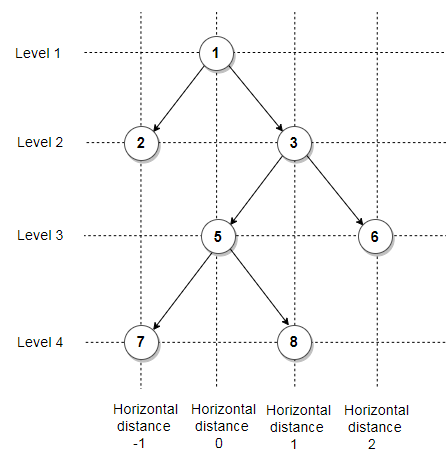
\includegraphics[scale=0.56]{pics/ht.png} 
\end{center}


	Diagonal, Given a binary tree, calculate the sum of all nodes for each diagonal having negative slope \. Assume that the left and right child of a node makes a 45–degree angle with the parent. \verb|https://www.techiedelight.com/find-diagonal-sum-given-binary-tree/|
\begin{lstlisting}[frame=single, language=c++]
// Recursive function to perform preorder traversal on the tree and
// fill the map with the diagonal sum of elements
 unordered_map<int, int> map;
void diagonalSum(Node* root, int diagonal, auto &map)
{
	// base case: empty tree
	if (root == nullptr) {
		return;
	}
	
	// update the current diagonal with the node's value
	map[diagonal] += root->data;
	
	// recur for the left subtree by increasing diagonal by 1
	diagonalSum(root->left, diagonal + 1, map);
	
	// recur for the right subtree with the same diagonal
	diagonalSum(root->right, diagonal, map);
}
	
\end{lstlisting}
\begin{description}
	\item[line 15] diagonal is just add 1 when you go to the left tree. Don't change when you go right tree. 
	\item[line 4] when you use sum of the whole tree, you must pass a reference type \texttt{auto\& map} here. 
\end{description}	

\begin{center}
	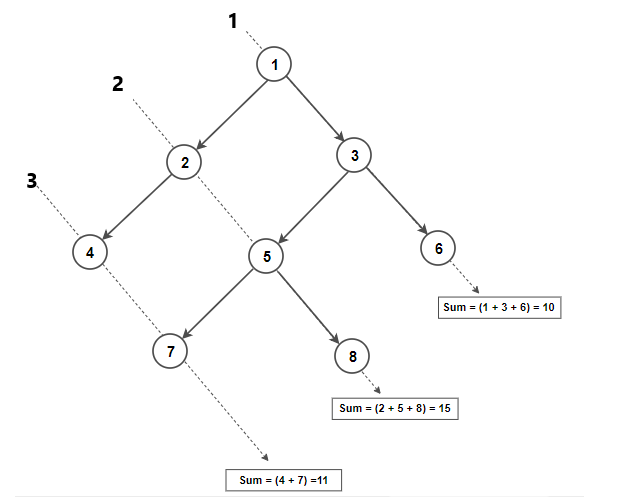
\includegraphics[scale=0.56]{pics/dt.png} 
\end{center}

 
\subsection{Search Tree}

	\par Search tree is the key in each node must be \textbf{greater than all keys stored in the left sub-tree, and smaller than all keys in the right sub-tree.} 

	\par Difference between BST and hash
\begin{itemize}
	\item So Hash Table seems to beating BST in all common operations. When should we prefer BST over Hash Tables? what are advantages? Following are some important points in favor of BSTs.
	
	\item We can get all keys in sorted order by just doing Inorder Traversal of BST. This is not a natural operation in Hash Tables and requires extra efforts.
	
	\item Doing order statistics, finding closest lower and greater elements, doing range queries are easy to do with BSTs. Like sorting, these operations are not a natural operation with Hash Tables.
	
	\item BSTs are easy to implement compared to hashing, we can easily implement our own customized BST. To implement Hashing, we generally rely on libraries provided by programming languages.
	
	\item With BSTs, all operations are guaranteed to work in O(Log(n) ) time. But with Hashing, O(1) is average time and some particular operations may be costly, especially when table resizing happens.
\end{itemize}

	\par ascending or descending order of BST. Pay attention here, they are all in order traversal.
\begin{lstlisting}[frame=single, language=c++]
void ascending(BST* root){
    if(root == NULL) return;
    ascending(root->left);
    std::cout<<root->data<<" ";
    ascending(root->right);
}
 
void descending(BST* root){
    if(root == NULL) return;
    descending(root->right);
    std::cout<<root->data<<" ";
    descending(root->left);
}
\end{lstlisting}


\subsection{Tree and recursion} 
\subsubsection{Base case}

	\par \textbf{Nearly all the tree problems can be resolved by recursive}. \textbf{Only focus on the current root logic.} For example, kth element problem, or lowest common ancester problem. The basic patter is below: 
	
\begin{lstlisting}[frame=single, language=c++]
TreeFun(root*...){
	BaseCase;
	TreeFun(root->Left...);
	TreeFun(root->right...);
	Join logic with current node according to different problem.
}	
\end{lstlisting}

	\par Global variables, reference variables, local variables, and return variables: differences in their usage within tree recursion programs

	\par 95\% Base Case is very simple.\textbf{Forgetting to check if the root is null. It's an important base case. In nearly all interview questions, the first statement inside recursive should be check root, then return nullptr, return 0 or return nothing.}


\begin{lstlisting}
if(root == nullptr){
	return ...
}	
\end{lstlisting}	

	\par The easier part is recursive all with left child and right child. At this time, you should design the recursive interface according to specific question. For example, If it is required from you to write a function that returns a value (e.g. the number of nodes in a binary tree), you have to make sure that the function actually "returns". One of the common mistakes is just writing the recursive call without writing the word "return" before it.

	\par The most difficult part is \textbf{Join}, You should write some logic here according to specific problem. For example, for the height of tree, we need to get max value of the left and right tree and increment it. 
\begin{lstlisting}[frame=single, language=c++]
int height(Node t){
	if(t == null)  {  
		return -1;   
	}
	else
	{
		int left = height(t->left);
		int right = height(t->right);
		//below are joint logic combine with current node
		int height = 1 + max( left, right );
		//put left and right recursive into assignment
		return height;
	}
}			
\end{lstlisting}		

	\par There are two problems involving returning nodes: one is finding the lowest common ancestor, and the other is deleting a node with a certain value from a BST. 
	
%	\par Binary tree recursive solutions can be divided into two thinking patterns. The first involves traversing the tree once to get the answer, and the second involves solving the problem by breaking it down. These two patterns correspond to the core frameworks of backtracking algorithms and dynamic programming, respectively.
	
	
	\par The inorder position is primarily used in BST (Binary Search Tree) scenarios, and you can consider the inorder traversal of a BST as traversing a sorted array.
	
	\par The preorder position doesn’t inherently have any special properties. The reason you find that many problems seem to involve writing code in the preorder position is simply because we tend to place code that isn’t sensitive to preorder, inorder, or postorder in the preorder position.

	\par You’ll notice that code in the preorder position executes from top to bottom, whereas code in the postorder position executes from bottom to top. This is significant because code in the preorder position can only access data passed from the parent node via function parameters, whereas code in the postorder position can access both parameter data and data returned from the subtrees via the function's return value.
	
	\par Can we obtain the solution by traversing the binary tree just once? If so, implement it using a traverse function along with external variables. This approach is called the "traversal" thinking pattern. Can we define a recursive function to derive the solution to the original problem using the answers from subproblems (subtrees)? If so, write the definition of this recursive function and fully utilize its return value. This is known as the "divide and conquer" thinking pattern. No matter which thinking pattern you use, you must consider:

\begin{itemize}

	\item If you isolate a single node of the binary tree, what does it need to do? When should it do it (preorder/inorder/postorder)? You don’t need to worry about other nodes—the recursive function will execute the same operation on all nodes.
	
	\item Differences between global variables, reference variables, local variables, and return variables when used in tree recursion programs.

	\item Referring back to the previous discussion: when encountering subtree problems, the first thing to consider is setting a return value for the function and focusing on postorder traversal.

	\item Conversely, if you’ve written a recursive-in-recursive solution like in the beginning, it’s likely worth considering whether it can be optimized using postorder traversal.

\end{itemize}



\subsubsection{Traversal Order}

\par Next big question is pre-order, in-order or post-order. \textbf{90\% we use post-order.} But it also depends on practical requirement.

\par In order examples:

\begin{itemize}
	
	\item inorder: two applications
	Find k’th smallest and k’th largest element in a BST:
\begin{lstlisting}[frame=single, language=c++]
int kthSmallest(Node* root, int *i, int k){
	if (root == nullptr) { // base case
		return INT_MAX;
	}
	
	int left = kthSmallest(root->left, i, k); // Left 
	
	if (left != INT_MAX) { // Join
		return left;
	}
	
	// if the current element is k'th smallest, return its value
	if (++*i == k) {
		return root->data;
	}
	
	return kthSmallest(root->right, i, k); // right
}
\end{lstlisting}
\begin{description}
	\item[source code] Only In order tranversal give ascending order, we have to use here. for example, kth element, you only think that the element in left tree, then return it, current root, then return it.  if it's in right tree, then recursive call with root->right. return INT\_MAX can be thought as a flag. if you want to look for a integer, you can use INT\_MAX to denote a flag. I should be shared by all recursive call, so we use pointer or reference here. 
\end{description}

	\item Print an expression tree
\begin{lstlisting}[frame=single, language=c++]
     *
   /  \
  +    c
 / \
a   b
	
void inorder(Node* root)
{
	if (root == nullptr) {
		return;
	}
	
	// if the current token is an operator, print open parenthesis
	if (isOperator(root->data)) {
		cout << "(";
	}
	
	inorder(root->left);
	cout << root->data;
	inorder(root->right);
	
	// if the current token is an operator, print close parenthesis
	if (isOperator(root->data)) {
		cout << ")";
	}
}
\end{lstlisting}

\end{itemize}

\par Pre order examples:


\begin{itemize}
	
\item Print left view of a binary tree
\begin{lstlisting}[frame=single, language=c++]
// Recursive function to print the left view of a given binary tree
void leftView(Node* root, int level, int &last_level)
{
	// base case: empty tree
	if (root == nullptr) {
		return;
	}
	
	// if the current node is the first node of the current level
	if (last_level < level)
	{
		// print the node's data
		cout << root->key << " ";
		
		// update the last level to the current level
		last_level = level;
	}
	
	// recur for the left and right subtree by increasing the level by 1
	leftView(root->left, level + 1, last_level);
	leftView(root->right, level + 1, last_level);
}
\end{lstlisting}


\end{itemize}

\par Post order examples:


\begin{itemize}
	\item Find maximum sum root to leaf path in a binary tree
\begin{lstlisting}[frame=single, language=c++]
// Function to calculate the maximum root-to-leaf sum in a binary tree
int getRootToLeafSum(Node* root){
	// base case: tree is empty
	if (root == nullptr) {
		return 0;
	}
	
	// calculate the maximum node-to-leaf sum for the left child
	int left = getRootToLeafSum(root->left);
	
	// calculate the maximum node-to-leaf sum for the right child
	int right = getRootToLeafSum(root->right);
	
	// consider the maximum sum child
	return (left > right? left : right) + root->data;
}	
\end{lstlisting}

\item combined:
find LCA
\begin{lstlisting}[frame=single, language=c++]
bool findLCA(Node* root, Node* &lca, Node* x, Node* y)
{
	// base case 1: return false if the tree is empty
	if (root == nullptr) {
		return false;
	}
	
	// base case 2: return true if either `x` or `y` is found
	if (root == x || root == y){  // 
		// set lca to the current node
		lca = root;
		return true;
	}
	
	// recursively check if `x` or `y` exists in the left subtree
	bool left = findLCA(root->left, lca, x, y);
	
	// recursively check if `x` or `y` exists in the right subtree
	bool right = findLCA(root->right, lca, x, y);
	
	// if `x` is found in one subtree and `y` is found in the other subtree,
	// update lca to the current node
	if (left && right) {
		lca = root;
	}
	
	// return true if `x` or `y` is found in either left or right subtree
	return left || right;
}
\end{lstlisting}
\begin{description}
	\item[] \textbf{Only focus on the current root logic}. If left anf right , then return root. otherwise just return left or right.  so simple!!
\end{description}

\end{itemize}

	\par Level order examples:
\begin{lstlisting}[frame=single, language=c++]
// Function to print spiral order traversal of a given binary tree
void spiralOrderTraversal(Node* root){
	if (root == nullptr) {
		return;
	}
	
	// create an empty double-ended queue and enqueue the root node
	list<Node*> deque;        // or use deque
	deque.push_front(root);
	
	// `flag` is used to differentiate between odd or even level
	bool flag = false;
	
	while (!deque.empty()) {  // loop till deque is empty
		// calculate the total number of nodes at the current level
		int nodeCount = deque.size();
		
		if (flag){ // print left to right
			// process each node of the current level and enqueue their
			// non-empty left and right child to deque
			while (nodeCount) {
				Node* curr = deque.front(); // pop from the front if `flag` is true
				deque.pop_front();
				
				cout << curr->key << " ";
				
				// it is important to push the left child into the back,
				// followed by the right child
				if (curr->left != nullptr) {
					deque.push_back(curr->left);
				}
				if (curr->right != nullptr) {
					deque.push_back(curr->right);
				}
				nodeCount--;
			}
		}
		else {  // print right to left
			// process each node of the current level and enqueue their
			// non-empty right and left child
			while (nodeCount){
				Node* curr = deque.back(); // it is important to pop from the back
				deque.pop_back();
				
				cout << curr->key << " ";    // print front node
				
				// it is important to push the right child at the front,
				// followed by the left child			
				if (curr->right != nullptr) {
					deque.push_front(curr->right);
				}			
				if (curr->left != nullptr) {
					deque.push_front(curr->left);
				}			
				nodeCount--;
			}
		}
		flag = !flag; // flip the flag for the next level
		cout << endl;
	}
}
\end{lstlisting}
\begin{description}
	\item[Source code] use BFS, so use queue, but we also need spiral, so have to use deque which support pop\_front and pop\_back. In order to print each level, use below source code pattern.
\begin{lstlisting}[frame=single, language=c++]
while (!deque.empty()){
	// calculate the total number of nodes at the current level
	int nodeCount = deque.size();	
	while(nodeCound){
		nodeCount--;
\end{lstlisting}	

\end{description}


	\par Traversal order summary 
\begin{itemize}
	\item Most of time, traversal order can be decided by the question itself very quickly.
	
	\item \textbf{Any time when you find Maximum or ancestor, this is a strong indication which we can use postorder.}
	
	\item You can combined use preorder visit and postorder logic combine together, such as LCA. 
\end{itemize}





\subsubsection{Interface}


	\par Next questions is interface design. (all auxiliary parameter) Find k’th smallest and k’th largest element in a BST:  \texttt{int *i} or \texttt{int\& i} is shared variable among all recursive. which record how many nodes we have visited so far. Return value is just your question answer. that is very easy to understand. 
	

	\par \textbf{If you change inside function, sometimes, you need to change it back when you return.}
\begin{lstlisting}[frame=single, language=c++]
// Recursive function to find paths from the root node to every leaf node
void printRootToleafPaths(Node* node, vector<int> &path){
	if (node == nullptr) { // base case
		return;
	}
	
	// include the current node to the path
	path.push_back(node->data);
	
	if (isLeaf(node)){ // if a leaf node is found, print the path
		for (int data: path) {
			cout << data << " ";
		}
		cout << endl;
	}
	
	// recur for the left and right subtree
	printRootToleafPaths(node->left, path);
	printRootToleafPaths(node->right, path);
	
	// backtrack: remove the current node after the left, and right subtree are done
	path.pop_back();
}	
\end{lstlisting}

	\par Another simple is use local stack variable. If you don't use reference, you don't need to pop\_back. That is not memory friendly solution, but you can avoid pop\_back function call. 
\begin{lstlisting}[frame=single, language=c++]
// Recursive function to find paths from the root node to every leaf node
void printRootToleafPaths(Node* node, vector<int> path){
	if (node == nullptr) {
		return;
	}
	
	path.push_back(node->data);
	
	// if a leaf node is found, print the path
	if (isLeaf(node))		{
		for (int data: path) {
			cout << data << " ";
		}
		cout << endl;
	}
	
	// recur for the left and right subtree
	printRootToleafPaths(node->left, path);
	printRootToleafPaths(node->right, path);
	
}		
\end{lstlisting}


	\par Information flow:
\begin{itemize}
	\item  return value from child to parent, (only return one value, so need some calculation inside from both left and right children)
	
	\item pass from parent to child, parameter to remember auto value(level) , 
	
	\item shared between children and parent. and pass a pointer parameter(max\_level) to remember static, which all recursive 
\end{itemize}
	








\subsubsection{Span child tree}

\par Determine whether the given binary tree nodes are cousins of each other. Two nodes of a binary tree are cousins if they have the same depth, but have different parents.   \textbf{traversal all, use global variable to store the good result when you traversal all. } 
\begin{lstlisting}[frame=single, language=c++]
// Perform inorder traversal on a given binary tree and update `x` and `y`
void inorder(Node* root, Node* parent, int level, NodeInfo &x, NodeInfo &y)
{
	// base case: tree is empty
	if (root == nullptr) {
		return;
	}
	
	// traverse left subtree
	inorder(root->left, root, level + 1, x, y);
	
	// if the first element is found, save its level and parent node
	if (root->key == x.key){
		x.level = level;
		x.parent = parent;
	}
	
	// if the second element is found, save its level and parent node
	if (root->key == y.key){
		y.level = level;
		y.parent = parent;
	}
	
	// traverse right subtree
	inorder(root->right, root, level + 1, x, y);
}	
\end{lstlisting}
\begin{description}
	\item[Source code] Use two global valure as reference, then search the whole tree. 
\end{description}



\subsubsection{Two trees}

	\par Recursive can be used to deal with two trees at the same time. 
\begin{lstlisting}[frame=single, language=c++]
	int identicalTrees(struct node* a, struct node* b){
		/*1. both empty */
		if (a==NULL && b==NULL)
		return true;
		
		/* 2. both non-empty -> compare them */
		if (a!=NULL && b!=NULL)    {
			return(
			a->data == b->data &&
			identicalTrees(a->left, b->left) &&
			identicalTrees(a->right, b->right)
			);
		} 
		
		/* 3. one empty, one not -> false */
		return false;
	} 
\end{lstlisting}	

	\par Some problems can be changed to two tree problems. such as if mirror. 

\begin{lstlisting}[frame=single, language=c++]
// Function to check if subtree rooted at `X` and `Y` mirror each other
bool isSymmetric(Node* X, Node* Y)
{
	// base case: if both trees are empty
	if (X == nullptr && Y == nullptr) {
		return true;
	}
	
	// return true if
	// 1. Both trees are non-empty, and
	// 2. The left subtree is the mirror of the right subtree, and
	// 3. The right subtree is the mirror of the left subtree
	return (X != nullptr && Y != nullptr) &&
	isSymmetric(X->left, Y->right) &&
	isSymmetric(X->right, Y->left);
}
\end{lstlisting}


	\par Fill any nodes next pointer:
\begin{lstlisting}[frame=single, language=c++]
Node connect(Node root) {
	if (root == null) return null;
	connectTwoNode(root.left, root.right);
	return root;
}

void connectTwoNode(Node node1, Node node2) {
	if (node1 == null || node2 == null) {
		return;
	}

	node1.next = node2;
	//sibling	
	connectTwoNode(node1.left, node1.right);
	connectTwoNode(node2.left, node2.right);
	//cousin
	connectTwoNode(node1.right, node2.left);
}
\end{lstlisting}
\begin{description}
	\item[Source code] \textbf{Any time you need to access cousin, you should use two nodes.} Three branch recursive, That is very different with others. 
\end{description}




\subsubsection{Traps}
\begin{itemize}
	\par You can check if one node is leaf node. The basic idea is just like to find if a value exist in the tree. But you can't ignore base case.
	
\begin{lstlisting}
      1    //must have base case to deal with this tree
    /   \     
  null   2


      1    //if (root->left == null && root->right == null) return;
    /   \  //can deal with this context. but can't deal with previous tree.
 null   null
 
int countLeaves(Node* t){ //an example of isLeaf
	if(t == null) 
		return 0;
	
	if(isLeaf(t))  {
		return 1;
	}
	else
		return countLeaves(t.left) +countLeaves( t.right);
}		
\end{lstlisting}		
	
	\item \textbf{Accessing the children values. You SHOULD NOT do that unless if want to judge if it's leaf node}. The child passed to the recursive call is treated as the new root. 
	
\end{itemize}



\subsubsection{Conclusion}

	\par According to question, if it will return a value, such as leaf count, height. It has to have a function return value. What value should we return? Usually, this is related to question. For example, kth element should return integer, LCA should return a pointer. At the same time, integer and pointer also can act as flag value. 

 
	\par The first statement always should be base case.
\begin{lstlisting}[breaklines]
if(root == nullptr) 
       return [value]
\end{lstlisting}

	
	
\begin{itemize}
	\item decide pre-order, in-order, and post-order. 

	\item For some easy problems, you have finished the problems. Then for some difficult problems, you need to some logic comparison or calculation. such as Maximum path sum in a binary tree. or max height tree.
	
	\item Logic inside the function, an good example is LCA: there are four different possible. 1) The root node is x or y, 2) the x or y only in left tree, 3) the x or y only in the right tree, 4) the x and y in the two separate tree. That is all the possibles, then write all logic to deal previous 4 possibles. 
	
	\item That is ALL!, never try to recursive call in your head. 
\end{itemize}

\begin{center}
	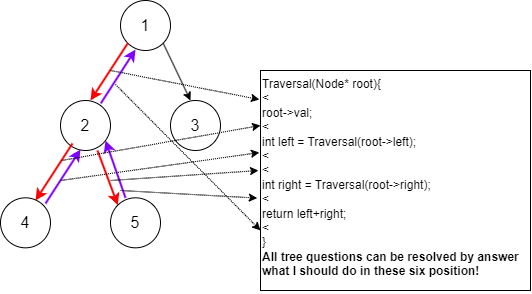
\includegraphics[scale=0.66]{pics/tree.drawio.png} 
\end{center}



\subsection{Interview questions}

\subsubsection{Print part of tree}

	\par \textbf{Usually use pre-order, then use some condition to suppress cout. At the same time, also need to pass some condition as parameter, (left view, level) return some flag(path include a node)}
	
	\par Print left view \textbf{When you return, the level will be local stack value, each value has stack scope.}

\begin{lstlisting}[frame=single, language=c++]
// Recursive function to print the left view of a given binary tree
void leftView(Node* root, int level, int &last_level)
{
	if (root == nullptr) { // base case: empty tree
		return;
	}
	
	// if the current node is the first node of the current level
	if (last_level < level){
		cout << root->key << " "; // print the node's data
		
		// update the last level to the current level
		last_level = level;
	}
	
	// recur for the left and right subtree by increasing the level by 1
	leftView(root->left, level + 1, last_level);
	leftView(root->right, level + 1, last_level);
}	
\end{lstlisting}	

	\par Print the certain level
\begin{lstlisting}[frame=single, language=c++]
// Function to print all nodes of a given level from left to right
bool printLevelLeftToRight(Node* root, int level)
{
	if (root == nullptr) {
		return false;
	}
	
	if (level == 1)
	{
		cout << root->key << " ";
		return true;  //return, don't go deeper to save time complexity.
	}
	
	// process left child before the right child
	bool left = printLevelLeftToRight(root->left, level - 1);
	bool right = printLevelLeftToRight(root->right, level - 1);
	
	return left || right;  //that is why we need to return bool. 
}

// Function to print level order traversal of a given binary tree
void levelOrderTraversal(Node* root)
{
	// start from level 1  till the height of the tree
	int level = 1;
	
	// run till printLevel() returns false
	while (printLevel(root, level)) {
		level++;
	}
}
\end{lstlisting}


	\par Print path include a node. If target is present in tree, then prints all the ancestors and returns true, otherwise returns false. 
	
\begin{itemize}
	\item The trick in this question is that it doesn't tell us the function should return bool, you should guess it out.
	
	\item preorder and postorder should be combined. when search key, use preorder, when print all ancester, use post order. 
	
	\item this combined order model also used in LCA.
\end{itemize}
\begin{verbatim}
      1
    /   \
   2      3
  /  \
 4     5
/
7
key is 7, then your function should print 4, 2 and 1.
\end{verbatim}

\begin{lstlisting}[frame=single, language=c++]
bool printAncestors(struct node *root, int target){
	/* base cases */
	if (root == NULL)
		return false;
	if (root->data == target)
		return true;
	
	/* If target is present in either left or right subtree of this node, then print this node */
	if ( printAncestors(root->left, target) ||
	printAncestors(root->right, target) ){
		cout << root->data << " ";
		return true;
	}
	/* Else return false */
	return false;
}	
\end{lstlisting}
\begin{description}
	\item[Source cde:] \textbf{Idea: just like max height example, return bool instead value, logic || instead max. the basic idea are quite same. }
	
	\item[Source code:] use return bool value to suppress cout
	
	\item[Source code:] \textbf{focuse local root} principal also can be used here. for local root, there are only three possibles.  current == target,  target in left tree, target in right tree.    
\end{description}

\subsubsection{Build tree}
	
	\par The problem of constructing a binary tree usually follows the "divide and conquer" approach: constructing the entire tree = root node + constructing the left subtree + constructing the right subtree.
	
	\par serialize and deserialize a tree
\begin{verbatim}
             11
            /   \
           /     \
          2       3
         /       / \
        /       /   \
       4       5     6
              / \
             /   \
            7     8
//11,2,4,.,.,.,3,5,7,.,.,8,.,.,6,.,.
\end{verbatim}


\begin{lstlisting}[frame=single, language=c++]
string serialize(Node* root) {  //serialize the root
	if (root == NULL) {
		return ".";   //a '.' character represents a null node
	}
	
	string serialized = "";
	
	serialized += to_string(root->key);  
	//add the current node to the serialized string then traverser its left and right children respectively
	
	serialized += "," + serialize(root->left);     //add the seperator after each node
	serialized += "," + serialize(root->right);
	
	return serialized;
}

Node* deserializeUtil(vector<string>& serialized, int& i) {
	
	if (i == serialized.size()) {   //if the whole array is exhausted
		return NULL;
	}
	
	string val = serialized[i++];
	
	if (val == ".") {   //if we encounter the '.' character => a null pointer
		return NULL;
	}
	//build the tree using the serialized array
	Node* node = new Node{ stoi(val) };
	
	node->left = deserializeUtil(serialized, i);
	node->right = deserializeUtil(serialized, i);
	
	return node;
	
}
\end{lstlisting}
\begin{description}
\item[Source code:] with nullptr(.) in string, we can use in-order unique define a tree.
\end{description}
	
	
	\par Construct a binary tree from inorder and preorder traversal.
	
\begin{lstlisting}[frame=single, language=c++]
Node* construct(int start, int end, vector<int> const& preorder,
int& pIndex, unordered_map<int, int>& map, int level){

	if (start > end) { // base case
		return nullptr;
	}
	
	// The next element in `preorder[]` will be the root node of subtree
	// formed by sequence represented by `inorder[start, end]`
	Node* root = newNode(preorder[pIndex++]);
	
	// get the root node index in sequence `inorder[]` to determine the
	// left and right subtree boundary
	int index = map[root->key];
	
	// recursively construct the left subtree
	for (int i = 0; i < level; ++i)
	cout << " ";
	cout << root->key << " " << start << " " << index << " " << end << endl;
	
	root->left = construct(start, index - 1, preorder, pIndex, map, level+1);
	
	// recursively construct the right subtree
	root->right = construct(index + 1, end, preorder, pIndex, map, level+1);
	
	// return current node
	return root;
}

// Construct a binary tree from inorder and preorder traversals.
// This function assumes that the input is valid
// i.e., given inorder and preorder sequence forms a binary tree
Node* construct(vector<int> const& inorder, vector<int> const& preorder){
	// get the total number of nodes in the tree
	int n = inorder.size();
	
	// create a map to efficiently find the index of any element in a given inorder sequence
	unordered_map<int, int> map;
	for (int i = 0; i < n; i++) {
		map[inorder[i]] = i;
	}
	
	// `pIndex` stores the index of the next unprocessed node in preorder;
	// start with the root node (present at 0th index)
	int pIndex = 0;
	
	return construct(0, n - 1, preorder, pIndex, map, 0);
}
//output 

        1
      /   \
     /     \
    2       3
    /      / \
   /      /   \
  4       5     6
         / \
        /   \
       7     8

1 0 2 7
 2 0 1 1
  4 0 0 0
 3 3 6 7
  5 3 4 5
   7 3 3 3
   8 5 5 5
  6 7 7 7
\end{lstlisting}
\begin{description}
	\item[Source code:] Iterate one time each time in pre-order.
	Build map to store in-order index, divide it into left tree and right tree. \textbf{just like quick\_sort}, pick an element from pre-order, then divide left and right according to index value in map
\end{description}

	\par How many BST?
\begin{lstlisting}
/* Main function, how many different BST tree given a number */ 
int numTrees(int n) {
	// Calculate the number of BSTs that can be formed from the closed interval [1, n]
	return count(1, n);
}

/* Calculate the number of BSTs that can be formed from the closed interval [lo, hi] */
int count(int lo, int hi) {
	if (lo > hi) return 1; // base case
	
	int res = 0;
	for (int i = lo; i <= hi; i++) {
		// Use the value of i as the root node
		int left = count(lo, i - 1);
		int right = count(i + 1, hi);
		// The total number of BSTs is the product of combinations of the left and right subtrees
		res += left * right;
	}	
	return res;
}	
\end{lstlisting}

\par Build BST
\begin{lstlisting}
/* Main function */
public List<TreeNode> generateTrees(int n) {
	if (n == 0) return new LinkedList<>();
	// Construct BSTs that can be formed from the closed interval [1, n]
	return build(1, n);
}

/* Construct BSTs that can be formed from the closed interval [lo, hi] */
List<TreeNode> build(int lo, int hi) {
	List<TreeNode> res = new LinkedList<>();
	// base case
	if (lo > hi) {
		res.add(null);
		return res;
	}
	
	// 1. Enumerate all possible root nodes.
	for (int i = lo; i <= hi; i++) {
		// 2. Recursively construct all valid BSTs for the left and right subtrees.
		List<TreeNode> leftTree = build(lo, i - 1);
		List<TreeNode> rightTree = build(i + 1, hi);
		// 3. Enumerate all combinations of left and right subtrees for the root node.
		for (TreeNode left : leftTree) {
			for (TreeNode right : rightTree) {
				// Use i as the value of the root node
				TreeNode root = new TreeNode(i);
				root.left = left;
				root.right = right;
				res.add(root);
			}
		}
	}
	
	return res;
}
\end{lstlisting}

\subsubsection{Change tree}

	\par Flatten tree. In order and post order are both OK, but preorder is not good.

\begin{lstlisting}[frame=single, language=c++]	
void flatten(struct Node* root){	
	if (root == NULL || root->left == NULL &&
	root->right == NULL) {
		return;
	}
	
	// if root->left exists then we have to make it root->right
	if (root->left != NULL) {
		flatten(root->left); // move left recursively
		
		// store the node root->right
		struct Node* tmpRight = root->right;
		root->right = root->left;
		root->left = NULL;
		
		// find the position to insert
		// the stored value  
		struct Node* t = root->right;
		while (t->right != NULL) {
			t = t->right;
		}
		
		t->right = tmpRight; // insert the stored value
	}
	
	// now call the same function for root->right
	flatten(root->right);
}
\end{lstlisting}

%\par Flatten A Binary Tree to Linked List (In-place) 
%Go down through the left, when right is not null, push right to stack. 

\begin{center}
	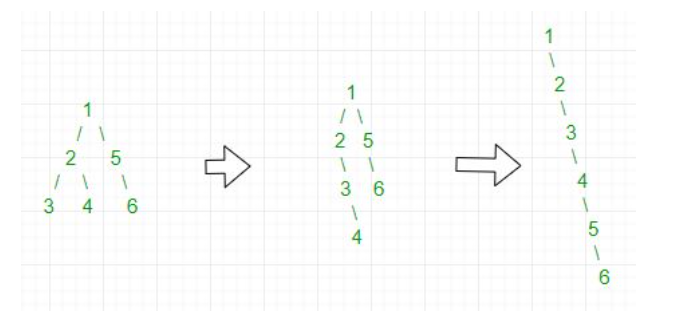
\includegraphics[scale=0.39]{pics/flat.png} 
\end{center}


	\par Truncate a binary tree to remove nodes that lie on a path having a sum less than k
\begin{itemize}
	\item Only node on a path, should use postorder. 
	\item Only print(or not print) or keep (or delete), should return bool
	\item calculate sum, should input a parameter sum
	\item \textbf{When delete leaf, parent will become leaf, That is why we have to use postorder}
	
	\item You have to use reference to pointer. 
\end{itemize}

\begin{lstlisting}
void trunc(Node* &curr, int k, int sum){
	if (curr == nullptr) { // base case: empty tree
		return;
	}
	
	// update sum of nodes in the path from the root node to the current node
	sum = sum + (curr->data);
	
	// Recursively truncate left and right subtrees
	trunc(curr->left, k, sum);
	trunc(curr->right, k, sum);
	
	// Since we are doing postorder traversal, the subtree rooted at the current
	// node may be already truncated, and the current node is a leaf
	// if the current node is a leaf node and its path from the root node has a sum
	// less than the required sum, remove it
	if (sum < k && isLeaf(curr)){
		
		delete(curr);  // free the memory allocated to the current node
		
		curr = nullptr; // set current node to null (node is passed by reference)
	}
};
\end{lstlisting}

	\par These two methods have common points: we both modify tree from bottom to top. When we modify current noe, we assume that all the child tree has finished. One use in-order, other use post-order. (Why? think about later.)



%\subsubsection{Traversal + other data structure}
%\begin{itemize}
%	\item Maximum Path Sum in a Binary Tree.(Global variable)
%	\begin{lstlisting}[breaklines]
%		For each node there can be four ways that the max path goes through the node:
%		1. Node only
%		2. Max path through Left Child + Node
%		3. Max path through Right Child + Node
%		4. Max path through Left Child + Node + Max path through Right Child
%		
%		The idea is to keep trace of four paths and pick up the max one in the end. An important thing to note is, root of every subtree need to return maximum path sum such that at most one child of root is involved. This is needed for parent function call. In below code, this sum is stored in 'max_single' and returned by the recursive function.
%	\end{lstlisting}
%\end{itemize}



\subsubsection{Other}

		
	\par Given the root of a binary tree, return all root-to-leaf paths in any order. ( you need root == nullptr, also need to judge if it's leaf node). That is an interesting example.  

\begin{lstlisting}
void pathTree(TreeNode* root, string path, vector<string> & result){
	if(root == nullptr){
		return;
	}
	if(path ==""){
		path = to_string(root->val);
	}
	else{
		path+="->";
		path+=to_string(root->val);
	}
	if(root->left == nullptr && root->right == nullptr){
		result.push_back(path);
		return;
	}
	
	pathTree(root->left, path, result);
	pathTree(root->right, path, result);
}

vector<string> binaryTreePaths(TreeNode* root) {
	string s = "";
	vector<string> result;
	pathTree(root, s, result);
	return result;
}
\end{lstlisting}


	\par In order without recursive, 
\begin{lstlisting}[frame=single, language=c++]
// An iterative process to print preorder traversal of Binary tree
void iterativePreorder(node *root){
    if (root == NULL) // Base Case
       return;
 
    // Create an empty stack and push root to it
    stack<node *> nodeStack;
    nodeStack.push(root);
 
    /* Pop all items one by one. Do following for every popped item
       a) print it
       b) push its right child
       c) push its left child
    Note that right child is pushed first so that left is processed first */
    while (nodeStack.empty() == false)    {
        // Pop the top item from stack and print it
        struct node *node = nodeStack.top();
        printf ("%d ", node->data);
        nodeStack.pop();
 
        // Push right and left children of the popped node to stack
        if (node->right)
            nodeStack.push(node->right);
        if (node->left)
            nodeStack.push(node->left);
    }
}
\end{lstlisting}

\par Idea: A common implementation of DFS, without check two unvisited condition. Because tree is a 1) minimally connected graph and having only one path between any two vertices. 2) no loop. 

%\item For search tree, look for lowest common ancestor(LCA). 
%\begin{lstlisting}[frame=single, language=c++]
%Node *LCA(Node *root, Node *p, Node *q) {
%  if (!root || !p || !q) return NULL;
%  if (max(p->data, q->data) < root->data)
%    return LCA(root->left, p, q);
%  else if (min(p->data, q->data) > root->data)
%    return LCA(root->right, p, q);
%  else
%    return root;
%}
%
%\end{lstlisting}

	\par Determine whether a binary tree is a subtree of another binary tree. both inorder and preorder together identify a tree quniquely.

	\par \textbf{Can be changed into a binary tree problem!}
	
\begin{itemize}
	\item print all subsequence, select current or don't select
	\item stair case, walk one or two
	\item house robbery
	\item All possible combine in array. 
	
\begin{lstlisting}[frame=single, language=c++]	
Input:  digits[] = { 1, 2, 2, 1 }	
{1, 2, 2, 1} 
{1, 2, 21} 
{1, 22, 1} 
{12, 2, 1} 
{12, 21} 
\end{lstlisting}
\end{itemize}



\section{Graph}
\subsection{Basic}

	\par A Tree is just a restricted form of a Graph. They fit with in the category of Directed Acyclic Graphs (or a DAG). So Trees are DAGs with the restriction that a child can only have one parent.

	\par Graphs are generally search breath first or depth first. The same applies to Tree.

	\par Basic represent way: \textbf{adjacency list} and \textbf{adjacency matrix}: 
\begin{center}
	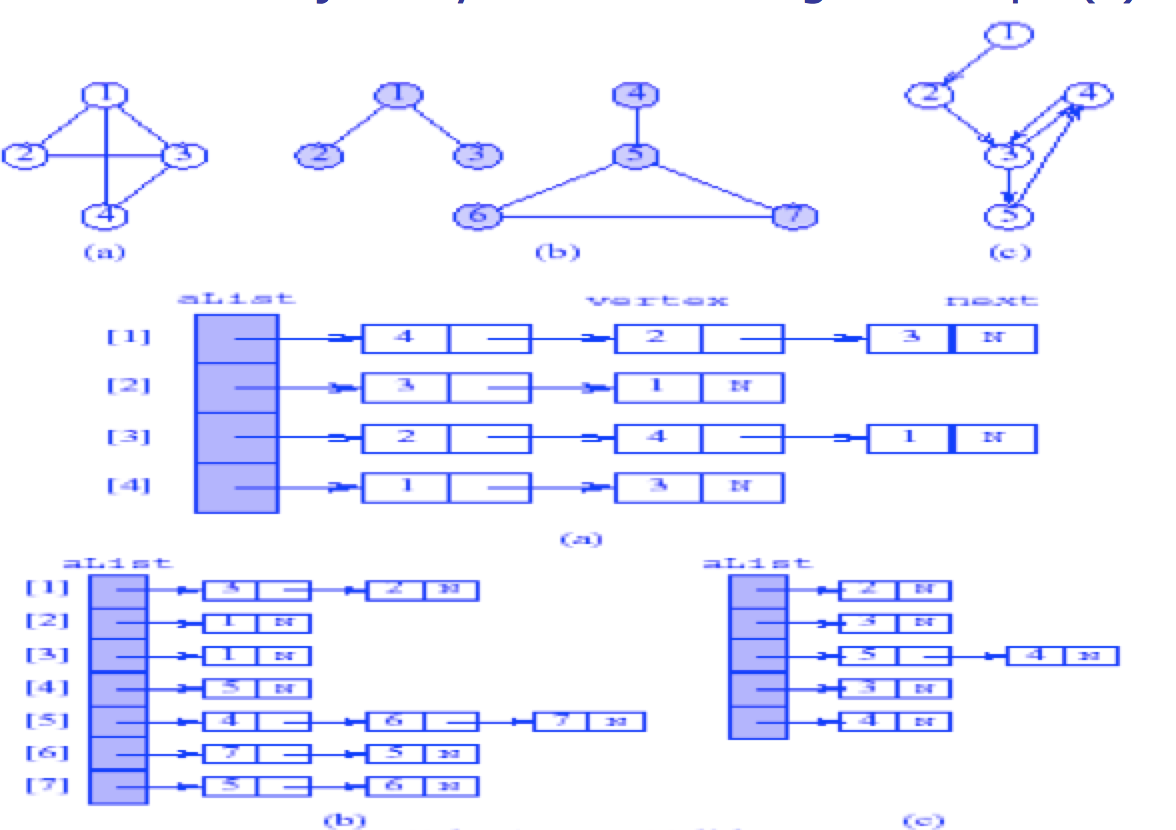
\includegraphics[scale=0.6]{pics/adjacency.png}
\end{center}


	\par You want to mirror the problem using a tree-like structure:For this we have boost graph library. The BGL currently provides two graph classes and an edge list adaptor: adjacency\_list, adjacency\_matrix and edge\_list.  The adjacency\_list class is the general purpose "swiss army knife" of graph classes.


\subsection{DFS and BFS}
\subsubsection{DFS}

	\par DFS has three versions 1) recursive 2) recursive to loop version. 3) uniform version.
	
\begin{itemize}
	
	\item Recursive version:
\begin{lstlisting}[frame=single, language=c++]
DFS(current){
  visit current;
  for all(next to current){
     if(unvisited(next)){
          DFS(next);
      }
   }
}
\end{lstlisting} 

\item Recursive to loop
\begin{lstlisting}[frame=single, language=c++]
DFS(start){
 S.push(start)  
  while(!S.empty()){
    current = top();
    visit current;
    If (current has one unvisited next){ 
         stack.push(next);
    }   
    else{
        stack.pop()
    }
}
}
\end{lstlisting} 

\item Unified version:
\begin{lstlisting}[frame=single, language=c++]
DFS(start){
 S.push(start)  
  while(!S.empty()){
    current = S.pop
    if(unvisited(current){
          visit current.
          for all(next to current and unvisited)
             S.push(next);
    }
  }
 }
\end{lstlisting} 
\end{itemize}

	\par  Why we need two "unvisited" words in DFS unified version.  
\begin{itemize}
\item When we pop node from S, then we visit it, then we add all adjacent nodes to S, In this way, When we pop 1 from S, we add 2, 3 to S. at this time, 3 is unvisited, then when we pop 2 from S, we will add 4, 3 to S. so there are two 3 in the S. 
\item Based on, we need to first unvisit to avoid visit 3 twice

\item When we reach 3; 1,2,4 have been visited, so when we want to add all 3 adjacent, we need second unvisited to avoid 1,2,4 to S.  
\end{itemize}
\begin{verbatim}
    1
  /   \
 2-----3
  \   /
    4      
\end{verbatim}

\par DFS is an algorithm to search a hierarchical structure. But, pre-order traversal seems to be something similar also. So, what is the difference between the two?? DFS says:
\begin{enumerate}
\item If element found at root, return success.
\item If root has no descendants, return failure
\item Recursive DFS on left subtree: success if element found
\item If not, Recursive DFS on right subtree: success if element found
\end{enumerate}

Pre-order Traversal says:
\begin{enumerate}
\item Visit the root
\item Recursive pre-order on left subtree
\item Recursive pre-order on right subtree
\end{enumerate}


\subsubsection{BFS}


\par There are two version of BFS:
\begin{itemize}
\item Form DFS unify version, We can change S(stack) to Q(queue) and get unified version. \textbf{That is why we call it unified version}
\begin{lstlisting}[frame=single, language=c++]
BFS(start){
 Q.push(start)  
  while(!Q.empty()){
    current = Q.pop
    if(unvisited(current){
          visit current.
          for all(next to current and unvisited)
             Q.push(next);
    }
  }
 }
\end{lstlisting} 

\item Common version:  Unified version will have multi-copy vertex in the queue. We can improve it as below:  1) when you add it to queue, visit it. In this way, avoid add multi-copy vertex in queue 2) Because All the vertex in queue is visited, when you pop it, you don't need to judge if it's visisted. 
\begin{lstlisting}[frame=single, language=c++]
DFS(start){
 D.push(start)  
  while(!D.empty()){
    current = D.pop  //2) no if here
    for all(next to current and unvisited){
         visit current.  //1) push and visit at the same time. 
         D.push(next);
     }
  }
 }
\end{lstlisting} 

\item conclusion:
\begin{enumerate}
	
\item  \textbf{Conclusion, just remember unified version. 1) pop current, push neighbor, 2) check two unvisited}
\item unified version will push two nodes into stack or queue, so for BFS, you can visit and push at the same time, in this way, you don't need to check current if it is unvisited. 

\item For DFS, you can't use this way, because you can only visit only one neighbor, or it will become BFS. so each time, you just push one node into stack. It leads to two other versions. recursive version, and loop version. 
\end{enumerate}


\end{itemize}

	\par Path is saved in the stack.  when you quit while loop. just pop up each position from stack, then you get a path. But for BFS, you need extra information to save parent information. 


\subsection{Spanning tree}

	\par 	BFS and DFS will produce spanning tree. 
	\par The minimum spanning tree can be obtained in polynomial time: Kruskal's algorithm, Prim's algorithm and Sollin's algorithm.


	\par Kruskal algorithm:
\begin{lstlisting}[frame=single, language=c++]
KRUSKAL(G):
 A = empty
 foreach v in G.V:
    MAKE-SET(v)
 foreach (u, v) ordered by weight(u, v), increasing:
    if FIND-SET(u) != FIND-SET(v):
       A = A  {(u, v)}
       UNION(u, v)
 return A
\end{lstlisting}
\begin{description}
	\item[Source code:] union find algorithm.
\end{description}


\subsection{Application}

	\par detect a cycle in the graph. \textbf{Undirected graph, not directed graph}.  The key point is just find visited[i], but if visited[i] is parent, then it's not a cycle. The whole logic is not complex. 

\begin{center}
	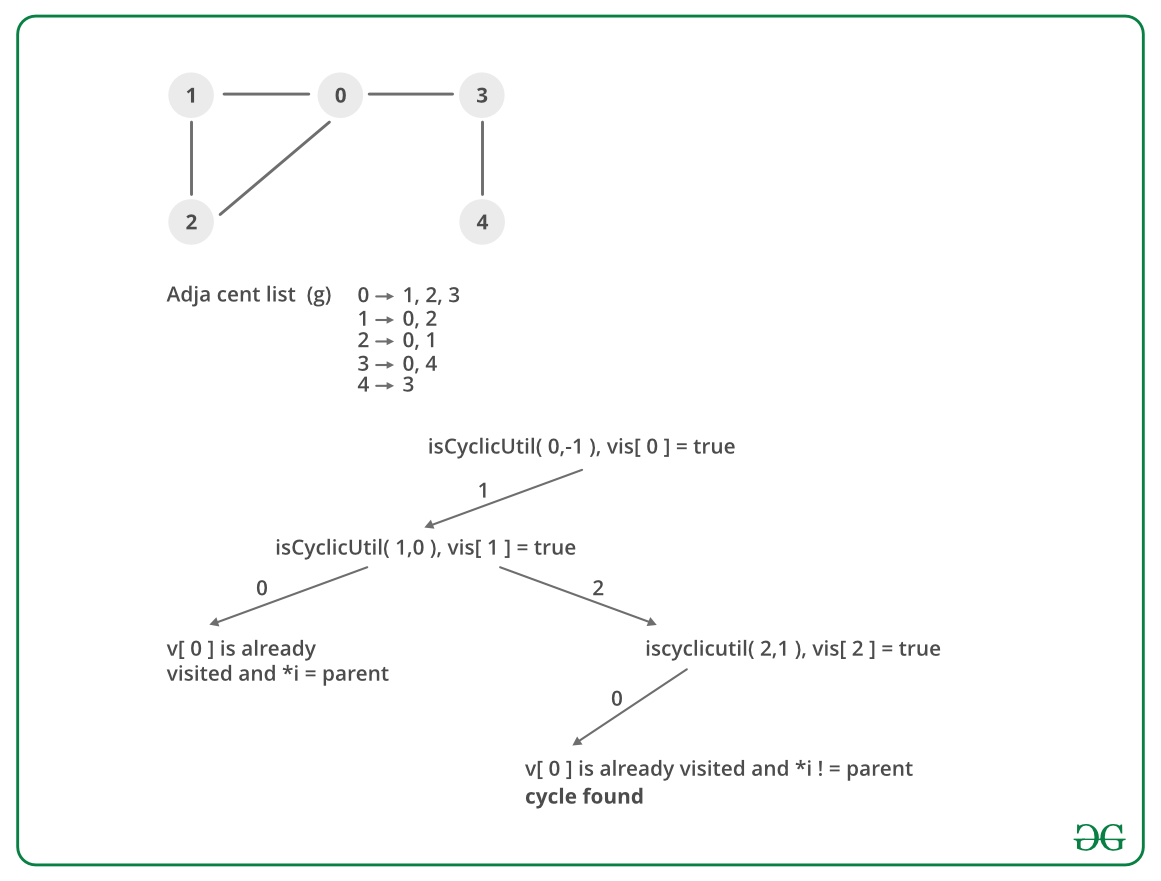
\includegraphics[width=0.7\linewidth]{pics/dc.png}
\end{center}

\begin{lstlisting}[frame=single, language=c++]
// A recursive function that uses visited[] and parent to detect
// cycle in subgraph reachable from vertex v.
bool Graph::isCyclicUtil(int v, bool visited[], int parent){
    visited[v] = true; // Mark the current node as visited
 
    // Recur for all the vertices adjacent to this vertex
    list<int>::iterator i;
    for (i = adj[v].begin(); i != adj[v].end(); ++i){
        // If an adjacent is not visited, then recur for that adjacent
        if (!visited[*i])        {
           if (isCyclicUtil(*i, visited, v))
              return true;
        }
//If an adjacent is visited and not parent of current vertex, then there is a cycle.
        else if (*i != parent)
           return true;
    }
    return false;
}
\end{lstlisting}



	\par Direct graph detect cycle. \textbf{need to add a onPath to detect cycle, different with undirected graph.} When we want to push node to stack, don't judge if we have visited them or not?  (undirected graph use visited[], directed graph use onPath[] )
	
\begin{lstlisting}
boolean[] onPath;
boolean[] visited;
boolean hasCycle = false;
void traverse(List<Integer>[] graph, int s) {
	if (onPath[s]) {
		// find cycle
		hasCycle = true;
	}
	if (visited[s] || hasCycle) {
		return;
	}
	visited[s] = true;

	onPath[s] = true;
	for (int t : graph[s]) {
		traverse(graph, t);
	}
	onPath[s] = false;
}
\end{lstlisting}



\section{Other customized data structure}

\subsection{union find}

	\par It is also called as "Online Equivalence class"
	
	\par definition of Equivalence relationship
	\begin{itemize}
		\item a ~ a. (Reflexivity)
		\item a ~ b if and only if b ~ a. (Symmetry)
		\item if a ~ b and b ~ c then a ~ c. (Transitivity)
	\end{itemize}
	
	\par online equivalence class, also known union-find question.  
	\begin{itemize}
		\item method 1: use array  
\begin{center}
	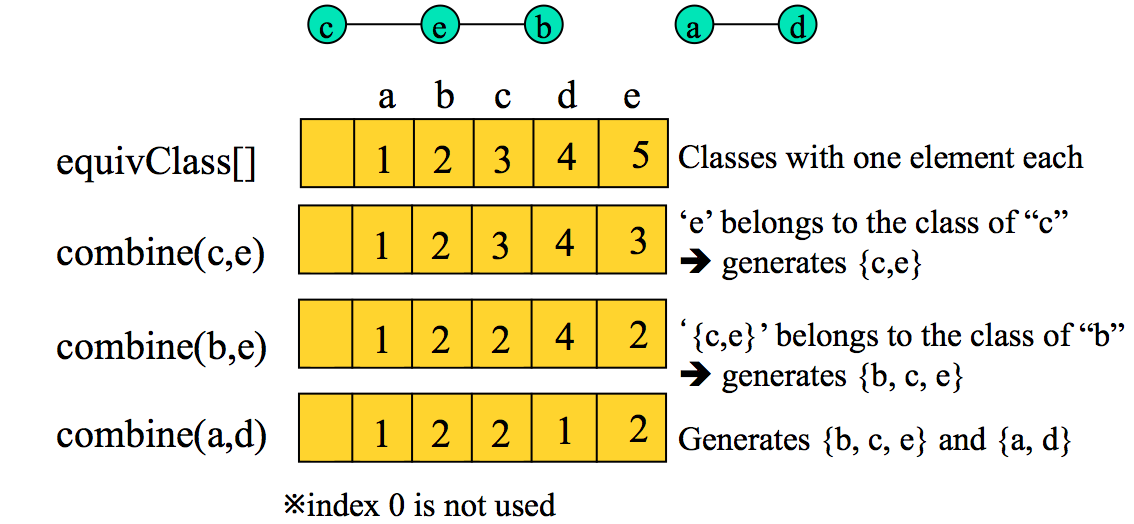
\includegraphics[scale=0.55]{pics/online_1.png} 
\end{center}
		
		
		\item method 2: stimulate pointer
\begin{center}
	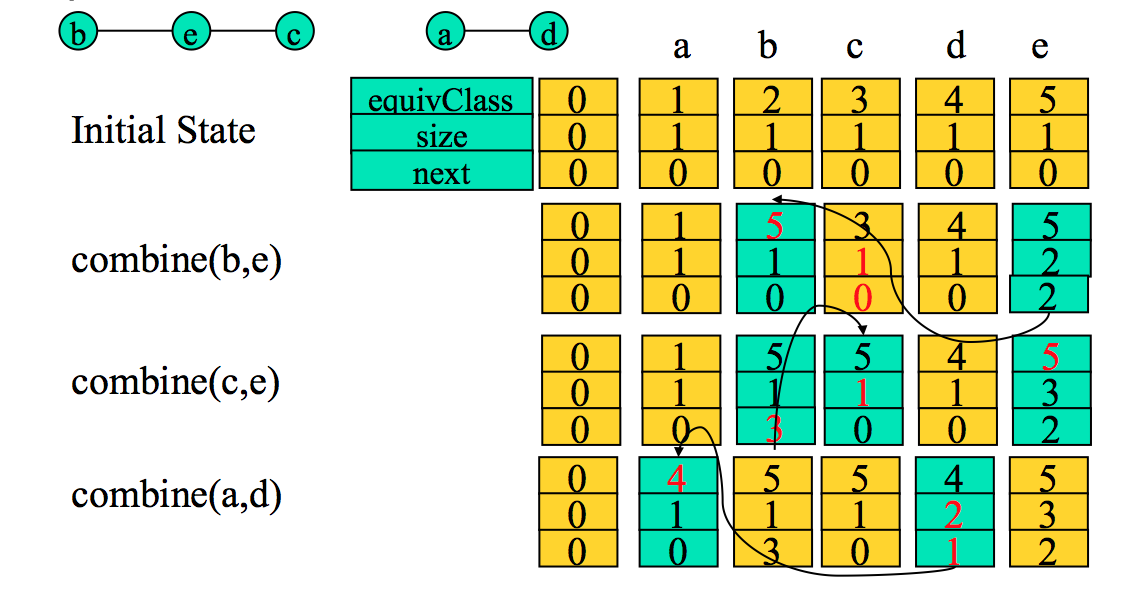
\includegraphics[scale=0.55]{pics/online_2.png}  
\end{center}

\begin{lstlisting}
class UF { 
	// Number of connected components
	private int count;
	// Stores the parent node of each node
	private int[] parent;
	
	// n is the number of nodes in the graph
	public UF(int n) {
		this.count = n;
		parent = new int[n];
		for (int i = 0; i < n; i++) {
			parent[i] = i;
		}
	}
	
	// Connects node p and node q
	public void union(int p, int q) {
		int rootP = find(p);
		int rootQ = find(q);
		
		if (rootP == rootQ)
			return;
		
		parent[rootQ] = rootP;
		count--;  // Merges two connected components into one
	}
	
	// Checks if node p and node q are connected
	public boolean connected(int p, int q) {
		int rootP = find(p);
		int rootQ = find(q);
		return rootP == rootQ;
	}
	
	public int find(int x) {
		if (parent[x] != x) {
			parent[x] = find(parent[x]);
		}
		return parent[x];
	}
	
	// Returns the number of connected components in the graph
	public int count() {
		return count;
	}
}
\end{lstlisting}
		
	\end{itemize}
	
	
\subsection{LRU and LFU}

	\par  LRU is hash + list. (listedhashmap)
	\par LFU is hash + heap. hashMap<key, pair{value, frequent}>. we still need key data structure to manage the frequency hashMap<frequent, hashLinkSet> freqToKeys.  freqToKeys is key to this question. 
	
	\par In LRU and LFU, The key data structure is LinkedHashMap, in LFU, it use LinkedSetMap, in fact, LinkedSetMap still use the LinkedHashMap behind the scene. 
\begin{center}
	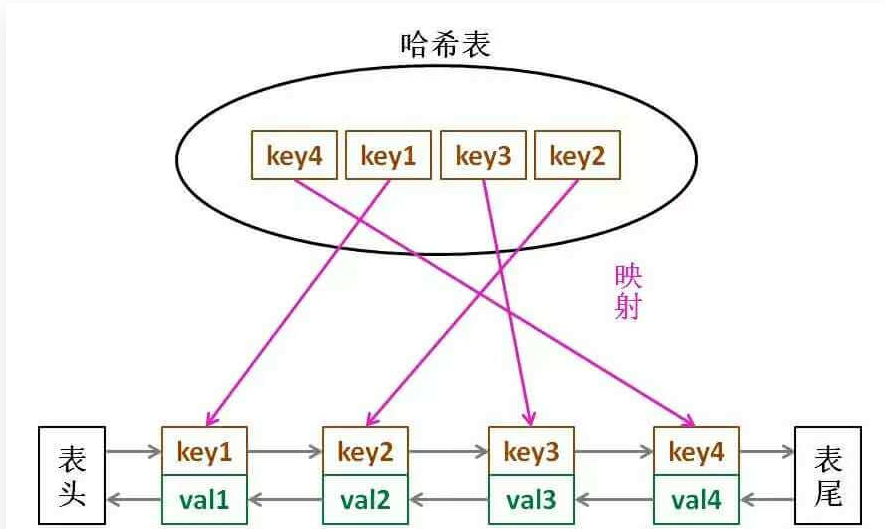
\includegraphics[width=0.7\linewidth]{pics/LinkedHashMap}
\end{center}
	
	
\subsection{O(1) insert, delete and getRandom}
Insert, delete get random O(1)  hash +vector(no need to keep vector sort). When you want to delete, swap it with the last element in the vector, then delete it.  \textbf{Most of complex data structure need hash + list/vector combine, it's a good clue}
	

\begin{itemize}
	
	\item C++ does not offer a collection template with the behavior that would mimic Java's LinkedHashMap<K,V>, so you would need to maintain the order separately from the mapping.
	
	This can be achieved by keeping the data in a std::list<std::pair<K,V>>, and keeping a separate std::unordered\_map<k,std::list<std::pair<K,V>>::iterator> map for quick look-up of the item by key:
	
	\begin{enumerate}
		\item On adding an item, add the corresponding key/value pair to the end of the list, and map the key to the iterator std::prev(list.end()).
		
		\item On removing an item by key, look up its iterator, remove it from the list, and then remove the mapping.
		
		\item On replacing an item, look up list iterator from the unordered map first, and then replace its content with a new key-value pair.
		
		\item On iterating the values, simply iterate std::list<std::pair<K,V>>.
	\end{enumerate}
	
	
\end{itemize}


\chapter{Algorithm}

	\par Big O notation. Remember below English words: constant, logarithmic (log n), linear (n)  linearithmic (n*log(n)) , quadratic $2^{n}$ (2 to the power of n), polynomial(quadratic cubic),  exponential $c^{n}$.  factorial $n!$.  O($10^{N}$): trying to break a password by testing every possible combination (assuming numerical password of length N).  traveling salesman problem(TSP)is factorial $n!$.  Both factorial and exponential are non-polynomial(NP). 

	\par verb|https://webusers.imj-prg.fr/~jan.nekovar/co/en/en.pdf| list some common mathematical English.  

	\par space complexity is much simple, usually, we only use O(1), O(n) and O($n^{2}$), we don't use other forms very often.  


\section{Math and geometry basic}
\subsection{Geometry}

	\par If three points make a triangle?
\begin{lstlisting}
// Calculation the area of triangle. We have skipped
// multiplication with 0.5 to avoid floating point computations
// if a is 0, don't make a triangle.
int a = x1 * (y2 - y3) + x2 * (y3 - y1) + x3 * (y1 - y2);
\end{lstlisting}

	\par Judge three points are in the same line?
\[
\dfrac{y_{2}-y_{1}}{x_{2}-x_{1}}  = \dfrac{y_{3}-y_{1}}{x_{3}-x_{1}}
\]

	\par Get one points in the triangle. 

\[
x = \dfrac{\dfrac{x_{1}+x_{2}}{2}+x_{3}}{2}
\]

\par If two rectangles overlap? l1: Top Left coordinate of first rectangle. r1: Bottom Right coordinate of first rectangle. l2: Top Left coordinate of second rectangle. r2: Bottom Right coordinate of second rectangle. 1) One rectangle is above top edge of other rectangle. 2) One rectangle is on left side of left edge of other rectangle.

\begin{lstlisting}[frame=single, language=c++]
// Returns true if two rectangles (l1, r1) and (l2, r2) overlap
bool doOverlap(Point l1, Point r1, Point l2, Point r2){
    // If one rectangle is on left side of other
    if (l1.x > r2.x || l2.x > r1.x)
        return false;
    // If one rectangle is above other
    if (l1.y < r2.y || l2.y < r1.y)
        return false;
    return true;
}
\end{lstlisting}


\subsubsection{Convex hull}

\begin{enumerate}
\item Find a point C that is inside the convex hull of S
( (sum of x coordinates)/ n, (sum of y coordinates)/n )
\item Sort S by polar angle and within polar angle by distance from C. Use atan2(y-Cy , x-Cx) c++ function.
\item Create a doubly linked circular list of points using above order
Let right link to the next point in the order and left link to the previous point

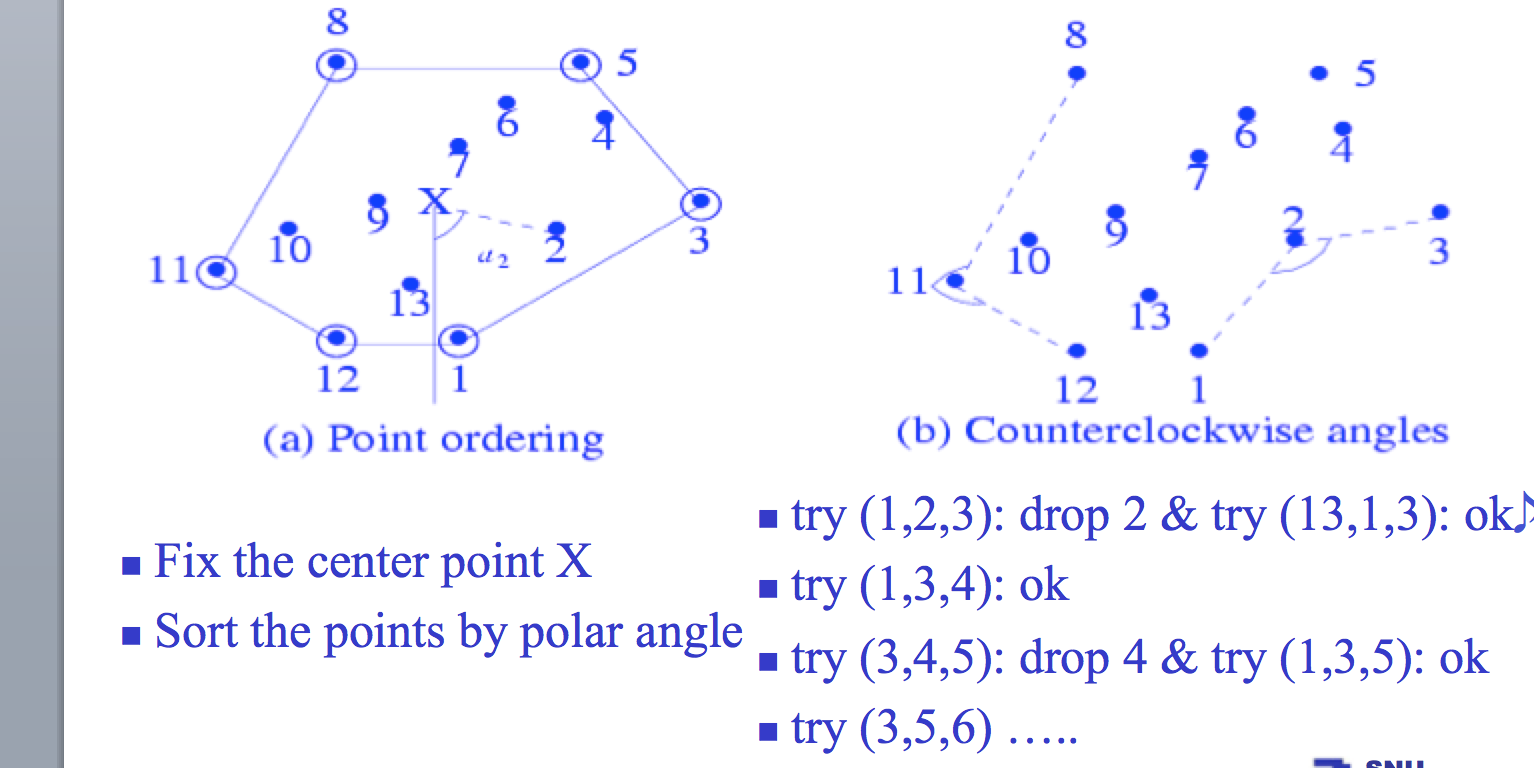
\includegraphics[scale=0.4]{pics/convex.png} \newline
\item Let p be the point that the smallest y-coordinate 
   (break a tie, if any, by selecting the one with largest x-coordinate)
   
\item use Law of cosines to calculate  angle formed by x, rx and rrx
\[
c^{2} = a^{2}+b^{2}-2ab\cos\lambda
\]

\begin{lstlisting}[frame=single, language=c++]
 for (x = p; rx = point to the right of x; x != rx) {
       rrx = point to the right of rx;
       if (angle formed by x, rx, and rrx is <=180 degrees) {
           delete rx from the list;
           rx = x; 
           x = point on left of rx;
       } 
       else { 
       x = rx; rx = rrx;}
   } 
\end{lstlisting}

\item For convex hull problem, you can use double link list to store all the extreme points. Because it need to use three consequence points to measure the degree to judge if it's less than 180 degrees. So double link list is the best data structure to use. 

\end{enumerate}


\subsection{Permutation and combination}

	\par repeated / unrepeated (Permutation/Combination)

	\par repeated permutation: Three number, how many permutation $10^3$. Another Three position, For each position, you can select 10 options and fill it.  If three position, For each position, you can selet 2 options and fill it. You get powerset problem $2^3$ \{a,b, c\} all the subset. 

	\par unrepeated permutation: $n! = factorial function$

	\par unrepeated combination:  
\begin{center}
	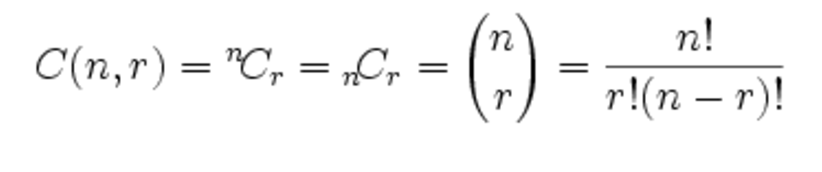
\includegraphics[scale=0.4]{pics/UC.png}
\end{center}	
 
	\par repeated combination: 
\begin{center}
	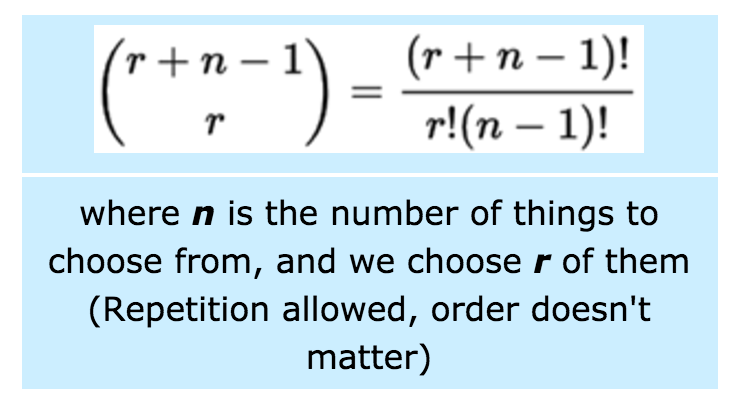
\includegraphics[scale=0.38]{pics/RC.png} 
\end{center}

	\par Detail can been seen here: https://www.mathsisfun.com/combinatorics/combinations-permutations.html




\subsection{Bit}

	\par Basic operations are: and, or, xor, not, right shift, left shit. 
\begin{lstlisting}[frame=single, language=c++]	
& | ^ ! << >> //six operators related with bits.

number |= 1UL << n; // set
number &= ~(1UL << n); //clear
number ^= 1UL << n;  //toggle, ^= can be used for toggle. 
\end{lstlisting}

	\par Many C compilers choose which right shift to perform depending on what type of integer is being shifted; often signed integers are shifted using the arithmetic shift, and unsigned integers are shifted using the logical shift.
	
\begin{lstlisting}[frame=single, language=c++]	
a|b|c|d //after we right shift, we change it to below
x|a|b|c
1) with a logical shift put 0 in x
2) with a arithmetic shift put a in x
\end{lstlisting}	
	
	\par XOR is exclusive or, You can think that it's subset of OR, for OR, if both bits are 1, the result is 1. but In XOR, we exclusive this possible,  You can think that it's "pure" or.  Based on previous definition. There are two characteristics:
\begin{lstlisting}
x^x = 0
x^0 = x
\end{lstlisting}
	from previous two examples, we can use it to find any number occur even number in the array. 
		
	\par change the last 1 to zeor. The basic idea is very interesting. 
\begin{lstlisting}[frame=single, language=c++]	
n&(n-1);
//110100-> 110000

//when we n-1: 110100, the right most 1 will become 0, all zeor after 
//right most 1 will become 1. 
110100
110011
*--	
\end{lstlisting}	
	
	\par Based on previous trip, we can test if a number is power of 2. There is only one 1 in the binary formation.
	
\begin{lstlisting}[frame=single, language=c++]	
bool isPowerOfTwo(int n) {
	if (n <= 0) return false;
	return (n & (n - 1)) == 0;
}		
\end{lstlisting}	
	
	\par Hamming weight,  Hamming weight of an integer is defined as the number of set bits in its binary representation. 
\begin{lstlisting}[frame=single, language=c++]	
int hammingWeight(uint32_t n) {
	int res = 0;
	while (n != 0) {
		n = n & (n - 1); //change n, you need to assign new value back to n. 
		res++;
	}
	return res;
}	
\end{lstlisting}	

	\par As noted in this answer, n\&(n-1) unsets the last set bit.
So, if we unset the last set bit and xor it with the number; by the nature of the xor operation, the last set bit will become 1 and the rest of the bits will return 0
\begin{lstlisting}
int set_bit = n ^ (n&(n-1));
\end{lstlisting}


\subsection{Usage of modulus \%}

\par Some applicatoin you can use with modulus (reminder).
\begin{itemize}
\item circular queue
\item hash
\item to know the last three digit. 
\end{itemize}

We usually use the % operator to calculate the modulus (remainder) to simulate a circular effect:
\begin{lstlisting}
int[] arr = {1,2,3,4,5};
int n = arr.length, index = 0;
while (true) {
	// Looping through a circular array
	print(arr[index % n]);
	index++;
}

int[] nextGreaterElements(int[] nums) {
	int n = nums.length;
	int[] res = new int[n];
	Stack<Integer> s = new Stack<>();
	// Doubling the array length to simulate a circular array
	for (int i = 2 * n - 1; i >= 0; i--) {
		// Modulo operation for index i, the rest follows the template
		while (!s.isEmpty() && s.peek() <= nums[i % n]) {
			s.pop();
		}
		res[i % n] = s.isEmpty() ? -1 : s.peek();
		s.push(nums[i % n]);
	}
	return res;
}	
\end{lstlisting}

\section{Two pointers}

\par two pointers are very popular algorithms in many 

\begin{center}
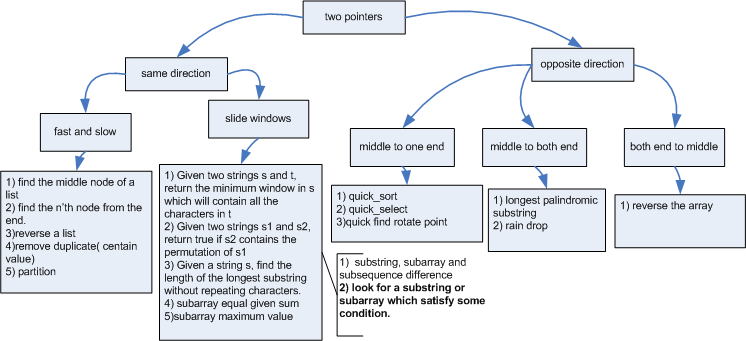
\includegraphics[scale=0.6]{pics/two_pointers.png}
\end{center}



\subsection{Middle to both ends}

	\par The longest palindrome substring
	
\begin{lstlisting}[breaklines]
string palindrome(string& s, int l, int r) {
	// check if it out boundary
	while (l >= 0 && r < s.size()
	&& s[l] == s[r]) {
		// both side move
		l--; r++;
	}
	// return result
	return s.substr(l + 1, r - l - 1);
}

string longestPalindrome(string s) {
	string res;
	for (int i = 0; i < s.size(); i++) {
		// s[i] is middle
		string s1 = palindrome(s, i, i);
		// s[i] and s[i+1] 
		string s2 = palindrome(s, i, i + 1);
		// res = longest(res, s1, s2)
		res = res.size() > s1.size() ? res : s1;
		res = res.size() > s2.size() ? res : s2;
	}
	return res;
}
\end{lstlisting}
	
	\par rain drop
	
\begin{lstlisting}[breaklines]
int trap(vector<int>& height) {
	if (height.empty()) return 0;
	int n = height.size();
	int res = 0;
	// memo
	vector<int> l_max(n), r_max(n);
	// base case
	l_max[0] = height[0];
	r_max[n - 1] = height[n - 1];
	// calculate l_max from left to right
	for (int i = 1; i < n; i++)
	l_max[i] = max(height[i], l_max[i - 1]);
	// calculate r_max from right to left
	for (int i = n - 2; i >= 0; i--) 
	r_max[i] = max(height[i], r_max[i + 1]);
	
	// calculate the last answer.
	for (int i = 1; i < n - 1; i++) 
	res += min(l_max[i], r_max[i]) - height[i];
	return res;
}
\end{lstlisting}



\subsection{slow and fast}

	\par remove duplicate
\begin{lstlisting}[breaklines]
int removeDuplicates(int[] nums) {
	if (nums.length == 0) {
		return 0;
	}
	int slow = 0, fast = 0;
	while (fast < nums.length) {
		if (nums[fast] != nums[slow]) {
			slow++;
			// maintain nums[0..slow] without duplicate
			nums[slow] = nums[fast];
		}
		fast++;
	}
	// length should be  + 1
	return slow + 1;
}
\end{lstlisting}

	\par partition
\begin{lstlisting}[breaklines]
template<class ForwardIt, class UnaryPredicate>
ForwardIt partition(ForwardIt first, ForwardIt last, UnaryPredicate p)
{
	first = std::find_if_not(first, last, p);
	if (first == last) return first;
	
	for (ForwardIt i = std::next(first); i != last; ++i) {
		if (p(*i)) {
			std::iter_swap(i, first);
			++first;
		}
	}
	return first;
}
\end{lstlisting}

	\par Note here, in removeDuplication, we ++ first, then assign, but in partition, we swap first, then ++. you need to know that slow pointer is pointing by these two methods. 

% remove and partition has the same idea, remove uses overwrite, partition uses swap, that is all. 
	

\subsection{slide windows}

	\par Code template of slide windows. Slide windows is suitable for some sub-string problem. 

\begin{lstlisting}[breaklines]
int left = 0, right = 0;

while (right < n) {`
	// increase windows
	window.add(a[right]);
	right++;
	
	//update windows
	//.......
	
	while (window needs shrink) {
		// decrease window
		window.remove(s[left]);
		left++;
		
		//update windows here.
		//......
	}
}			
\end{lstlisting}

	\par An example. minimal substring in source which includes all the letters of in target. leetcode 76.
	s = "ADOBECODEBANC", t = "ABC, output "BANC"
\begin{lstlisting}
string minWindow(string s, string t) { 
	unordered_map<char, int> need, window;
	for (char c : t) need[c]++;
	
	int left = 0, right = 0;
	int valid = 0;
	// Variables to record the starting index and length of the minimum window substring
	int start = 0, len = INT_MAX;
	while (right < s.size()) {
		// `c` is the character that will enter the window
		char c = s[right];
		right++; 	// Expand the window
		if (need.count(c)) { // Update the data inside the window
			window[c]++;
			if (window[c] == need[c])
			valid++;
		}
		
		// Check if the left side of the window needs to shrink
		while (valid == need.size()) {
			// Update the minimum window substring here
			if (right - left < len) {
				start = left;
				len = right - left;
			}
			// `d` is the character that will exit the window
			char d = s[left];
			// Shrink the window
			left++;
			// Update the data inside the window
			if (need.count(d)) {
				if (window[d] == need[d])
				valid--;
				window[d]--;
			}                    
		}
	}
	// Return the minimum window substring
	return len == INT_MAX ? "" : s.substr(start, len);
}
\end{lstlisting}
	

\section{Recursive}
\subsection{Basic}

	\par Consider an array/string: \texttt{{1,2,3,4}}
\begin{lstlisting}
Subarray: contiguous sequence in an array i.e.{1,2},{1,2,3}

Subsequence: Need not to be contiguous, but maintains order i.e. {1,2,4}

Subset: Same as subsequence except it has empty set i.e. {1,3},{}

Given an array/sequence of size n, possible
Subarray = n*(n+1)/2
Subseqeunce = (2^n) -1 (non-empty subsequences)
Subset = 2^n
\end{lstlisting}
	

	\par recursive is not an algorithm, it's just a method. D\&C, DP, backtrack, bound and boundary all use recursive in their implementation, but different ways. 
	
	\par First, the inline specification on a function is just a hint. The compiler can (and often does) completely ignore the presence or absence of an inline qualifier. With that said, a compiler can inline a recursive function, much as it can unroll an infinite loop. It simply has to place a limit on the level to which it will "unroll" the function.

	\par One recursive(Factorial),  Two recursive call( Hanoti) (Tree), Multi Recursive (Permutation)

	\par result is single (Factorial), Result is many steps,(Hanoti) (Maze), Result is a set( permutation). you can see that 1) any recursive function should at least one input parameter, and this parameter should to be pass sub-problem. 2) for return value, it has two different kind, if result is single value, you should return a value, such as Factorial. If result is set(permutation) or many steps(in-order traversal of treeor Hanoi tree), you can declare your function as void. 3) Some functions need input another parameter, such as level information in the tree or position information in the permutation. 4) Base case can be understood differently, most of time base case is 0 or null, but for permutation, base case is i==n.  most subproblem, i decrease, but for permutation, for each subproblem i increase. 
	
\begin{itemize}
\item single result 
\begin{lstlisting}[frame=single, language=c++]
int Factorial(int n){
if (n == 1) 
     return 1;
 return n*Factorial(n-1);
}
\end{lstlisting}

	\item result is serial steps (Hanoti) DFS(Maze)
\begin{lstlisting}[frame=single, language=c++]
FUNCTION MoveTower(disk, source, dest, spare):
IF disk == 0, THEN:
    move disk from source to dest
ELSE:
    MoveTower(disk - 1, source, spare, dest)   // Step 1 above
    move disk from source to dest              // Step 2 above
    MoveTower(disk - 1, spare, dest, source)   // Step 3 above
END IF
\end{lstlisting}

	\item  Result is a set( permutation)

\end{itemize}

	\par It includes direct recursive and indirect recursive. direct recursive is R() call R() again in it's funciton body. It has two parts: \textbf{1)base and 2) recursive component}


\subsection{Solution space }

\par Why this basic conception is so important, Because you can use these four to describe solution space. repeated permutation can be use in 0/1 backpack problem.  LCS problem.  

\par Nearest point pair's solution space is n*(n-1). It's $n^2$. A good hint is that it can be reduce $n*log(n)$. So We should consider D\&C (divide and conquer)

\par 0/1 packback's solution's space is $2^n$, A good hint is that I can be reduce to $n^c$. (c is constant) by dynamic programming. 

\par If there is not D\&C or DP, you have to use branch and bound or backtracking. Such as TSP traveling sales problem

\par If you need optimal answer, You need to traversal the whole solution space. ( such as TSP and 0/1 backpacking). If you don't need optimal answer, you don't need to do that, In these two conditions, you all need to \textbf{backtracking.}

\par Why I can't use DP to TSP, but I can use DP to 0/1?  

\par Recursion is a mathematical induction. 

\par Modeling is mapping your problem to a abstract structure.

\begin{itemize}
	\item Permutation: arrangement, tour, ordering sequence
	\item subset: cluster, collection, committee, group, packaging, selection
	\item tree:hieracrchy, dominance, ancestor/descendant, taxonomy
	\item graphs: network, circuit, web, relationship
	\item points
	\item polygon
	\item string 
\end{itemize}

\par Some typical applications, you need to remember them.
\begin{itemize}
	\item 5 cities, TSP, time complexity is n! (5! = 120)
	
	\item 5 number, whole set partition.  bell number, for 5, last result is 42. please see set partition number in recursive section.
	
	\item 5 object, 0/1 backpack,  Subset, time complexity is $2^n$ ($2^5$=32)
	
	\item 5 icecream, 3 spoon,  combination, (c(5, 3) = 10). combination is subset(number of element is 3) of subset, they are different. 
	
\end{itemize}
	
	
\subsection{Basic recursive pattern}

	\par You should understand Big O here. For example:
	\begin{itemize}
		\item O(n) is found max and min
		
		\item O(n*n) is bubble sort
		
		\item O(n*n*n) is solutions for a multi-variable equation: 3x+4y+5z = 108, then get all x, y z.
		
		\item O(n*logn) is quick sort. binary search. 
		
		\item O($2^{n}$) print all subsequences
		
		\item catalan number. print all parentheses.
		
		\item O($n!$) print all permutation.
	\end{itemize}
		
	\par Print all subsequences, why is power(2,n)?

\begin{lstlisting}[frame=single, language=c++]
void sub(string& s, int i, int j, string res) {
	if (i == j) {
		cout << res << endl;
		return;
	}
	sub(s, i + 1, j, res); //don't select current character
	
	res.push_back(s[i]); //select current character.
	sub(s, i + 1, j, res);
}	
\end{lstlisting}	
	
	\par We can use another method to resolve this quesiton. That is bucket perspective, above code is ball perspective. 
	
\begin{lstlisting}
void backtrack(int[] nums, int start) {	
	// pre-order, every node is a subset. such as, empty subset[]
	res.add(new LinkedList<>(track));

	for (int i = start; i < nums.length; i++) {
		track.addLast(nums[i]); // make a choice
		
		// Control the traversal of branches using the start parameter to avoid generating duplicate subsets.
		backtrack(nums, i + 1);
		
		track.removeLast(); // revoke a choice
	}
}
\end{lstlisting}
	
	In this tree, each edge is choice, each node is an answer, for n = 3, there are 8 nodes in below graph. We call it back track tree. 
	


\begin{minipage}{.5\textwidth}		
	\begin{center}
		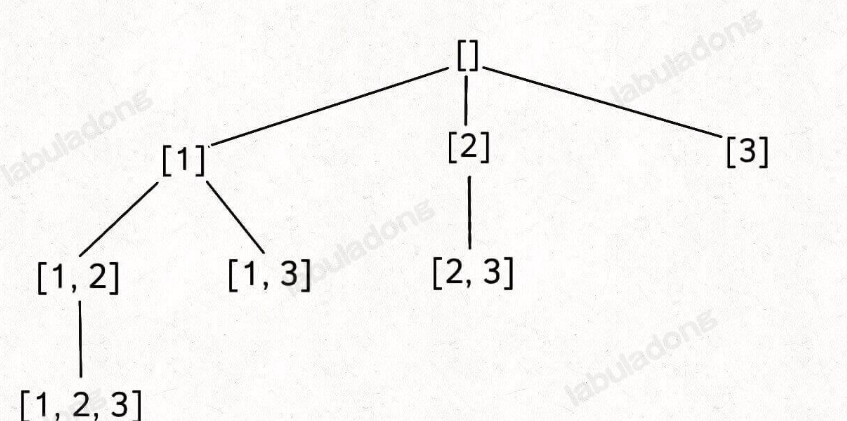
\includegraphics[width=0.9\linewidth]{pics/path1.png} 
	\end{center}
\end{minipage}	
\begin{minipage}{.5\textwidth}		
	\begin{center}
		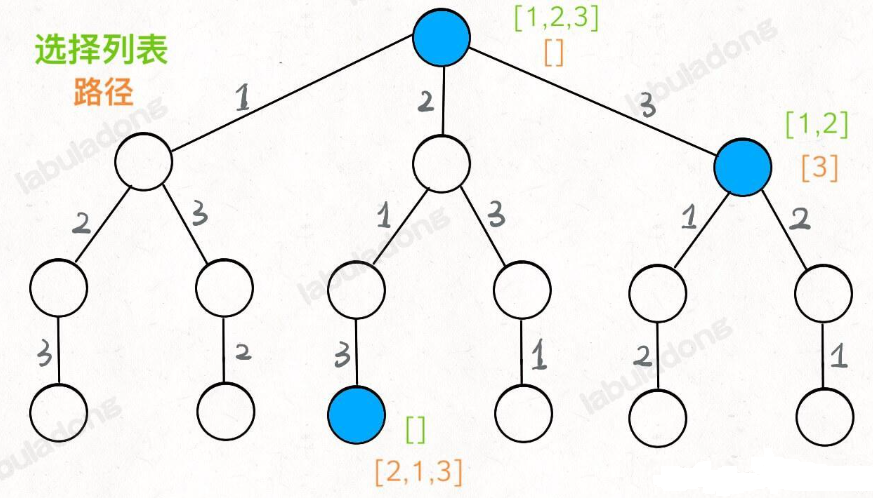
\includegraphics[width=0.9\linewidth]{pics/path.png}
	\end{center}
\end{minipage}	
		
	\par A similar idea is to LIS problem. it's also $2^n$
	you can think in this way, previous one is 2*f(n-1), below is f(n-1) f(n-2)...f(1)
	but f(n-2)...f(1) is just another f(n-1), so equal 2*f(n-1). Detail is we have a lot of overlap problem.
	Time complexity is power(2,n) The time complexity of this recursive approach is exponential as there is a case of overlapping subproblems as explained in the recursive tree diagram above.
	\begin{center}
		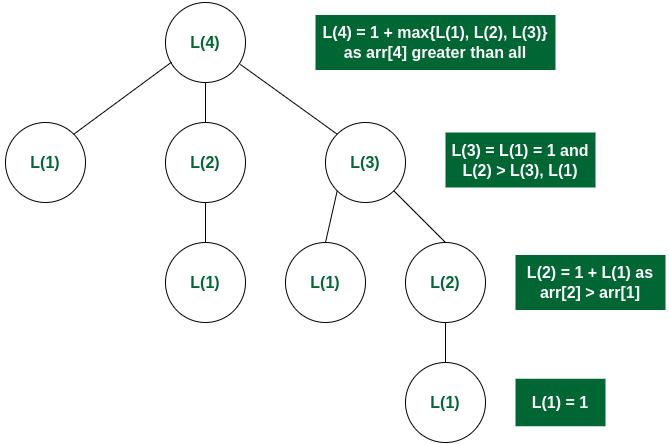
\includegraphics[width=0.5\linewidth]{pics/lis}
	\end{center}
	
\begin{lstlisting}[frame=single, language=c++]
int _lis( int arr[], int n, int *max_ref){
	if (n == 1) /* Base case */
	return 1;
	
	// 'max_ending_here' is length of LIS ending with arr[n-1]
	int res, max_ending_here = 1;
	
	/* Recursively get all LIS ending with arr[0],
	arr[1] ... arr[n-2]. If arr[i-1] is smaller
	than arr[n-1], and max ending with arr[n-1]
	needs to be updated, then update it */
	for (int i = 1; i < n; i++){
		res = _lis(arr, i, max_ref);
		if (arr[i-1] < arr[n-1] && res + 1 > max_ending_here)
		max_ending_here = res + 1;
	}
	
	// Compare max_ending_here with the overall max. And update the overall max if needed
	if (*max_ref < max_ending_here)
		*max_ref = max_ending_here;
	
	// Return length of LIS ending with arr[n-1]
	return max_ending_here;
}	
\end{lstlisting}	
	
	
	\par If the answer is one, such as LIS, the result should be in the root node, we should use post order, If the answer are a lot , the result shoudl be in leaf node, we should use base case. such as all possible subsequence. 
	
	
	\par Given a set A = {1, 2, 3, . . ., n }. It is called a partition of the set A if the following conditions follow: 1) The union of all the sets is the set A. 2) The intersection of any two sets is an empty set.

\begin{center}
	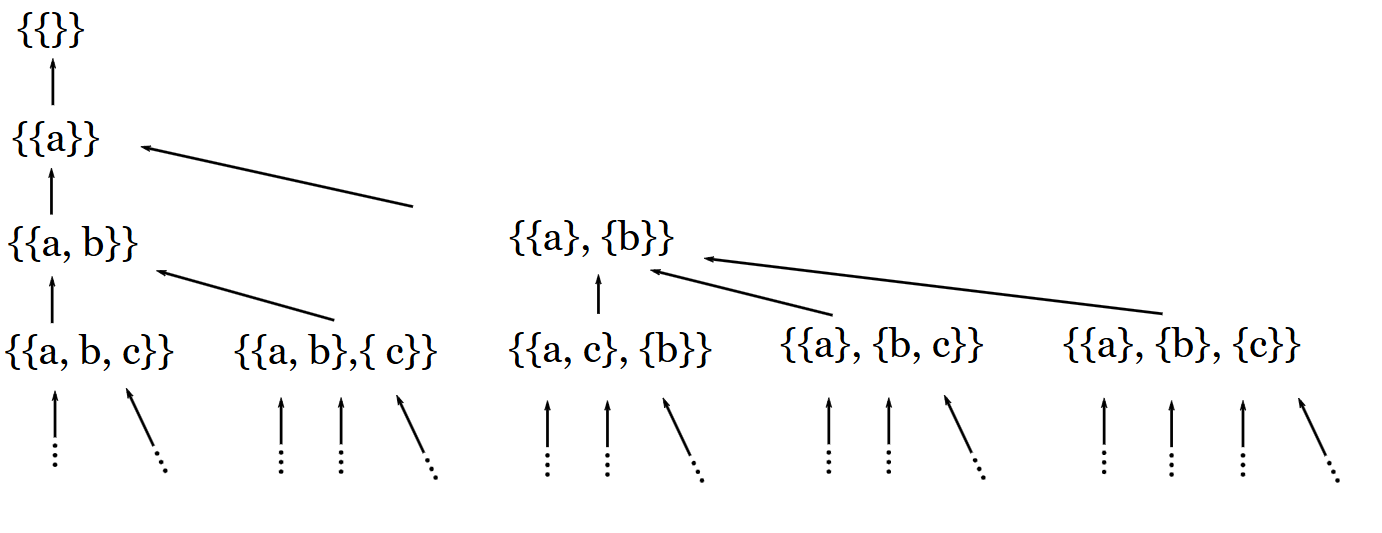
\includegraphics[scale=0.25]{pics/bell.png}
\end{center}
	
\begin{lstlisting}
// Function to print a partition
void printPartition(vector<vector<int> > ans)
{
	for (auto i : ans) {
		cout << "{ ";
			for (auto element : i) {
				cout << element << " ";
			}
			cout << "} ";
	}
	cout << endl;
}

// Function to generate all partitions
void Partition(vector<int> set, int index, vector<vector<int> >& ans){
	
	// If we have considered all elements in the set print the partition
	if (index == set.size()) {
		printPartition(ans);
		return;
	}
	
	// For each subset in the partition add the current element to it and recall
	for (int i = 0; i < ans.size(); i++) {
		ans[i].push_back(set[index]);
		Partition(set, index + 1, ans);
		ans[i].pop_back();
	}
	
	// Add the current element as a singleton subset and recall
	ans.push_back({ set[index] });
	Partition(set, index + 1, ans);
	ans.pop_back();
}

// Function to generate all
// partitions for a given set
void allPartitions(vector<int> set){
	vector<vector<int> > v;
	Partition(set, 0, v);
}


int main(){
	int n = 5;
	vector<int> set(n);
	for (int i = 0; i < n; i++) {
		set[i] = i + 1;
	}
	
	// Generate all partitions of the set
	allPartitions(set);
	return 0;
}
\end{lstlisting}

\begin{lstlisting}
{ 1 2 3 4 5 } 
{ 1 2 3 4 } { 5 } 
........
{ 1 2 4 } { 3 5 } 
{ 1 } { 2 } { 3 } { 4 } { 5 } 
\end{lstlisting}
	
	\par Catalan number, all possible parentheses combination. (It's not good implementation, some child problems have been calcualted many time.  You should use dynamic programming to remember the child problems result. but child program result is very big.  It's a question for ALL , not for ONE result. So backtrace algorithm is more good for this questions. 
	
	\par Re-interpreting the symbol X as an open parenthesis and Y as a close parenthesis, Cn counts the number of expressions containing n pairs of parentheses which are correctly matched:
\begin{lstlisting}
	((()))     (()())     (())()     ()(())     ()()()
\end{lstlisting}	
	
	Cn is the number of different ways n + 1 factors can be completely parenthesized (or the number of ways of associating n applications of a binary operator, as in the matrix chain multiplication problem). For n = 3, for example, we have the following five different parenthesizations of four factors:
	
\begin{lstlisting}	
	((ab)c)d    (a(bc))d    (ab)(cd)     a((bc)d)     a(b(cd))
\end{lstlisting}	
	
\begin{lstlisting}[frame=single, language=c++]
vector<string> ap(string& s, int i, int j) {
	vector<string> result;
	if (i == j-1 && i<s.size()) {
		result.push_back(s.substr(i,1));
		return result;
	}
	for (int k = i; k < j-1; ++k) {
		vector<string> v1 = ap(s, i, k+1);
		vector<string> v2 = ap(s, k+1 , j);
		
		string rs;
		for (auto e : v1) {
			for (auto e1 : v2) {
				rs = "(";
				rs +=  e;
				rs += e1;
				rs += ")";
				result.push_back(rs);
			}
		}
	}
	return result;
}

string s = "abcd";
auto com = ap(s, 0, 4);

for (auto e : com) {
	cout << e << endl;
}

(a(b(cd)))
(a((bc)d))
((ab)(cd))
((a(bc))d)
(((ab)c)d)	
\end{lstlisting}	
	
	\par The same idea is to build binary search tree
	
\begin{lstlisting}[frame=single, language=c++]
// Recursive function to return a list of tree pointers of all possible
// binary trees having the same inorder sequence as `in[start, end]`
vector<Node*> generateBinaryTrees(vector<int> &in, int start, int end)
{
	// create an empty list to store the root of the constructed binary trees
	vector<Node*> trees;
	
	// base case
	if (start > end)
	{
		trees.push_back(nullptr);
		return trees;
	}
	
	// consider each element in the inorder sequence as the root
	for (int i = start; i <= end; i++)
	{
		// recursively find all possible left subtrees for root `i`
		vector<Node*> left_subtrees = generateBinaryTrees(in, start, i - 1);
		
		// recursively find all possible right subtrees for root `i`
		vector<Node*> right_subtrees = generateBinaryTrees(in, i + 1, end);
		
		// do for each combination of left and right subtrees
		for (Node* l: left_subtrees)
		{
			for (Node* r: right_subtrees)
			{
				// construct a binary tree with i'th element as the root and whose
				// left and right children point to `l` and `r`, respectively
				Node* tree = new Node(in[i], l, r);
				
				// add this tree to the output list
				trees.push_back(tree);
			}
		}
	}
	
	return trees;
}	
\end{lstlisting}	
	
	
	
\begin{lstlisting}
void subset(int arr[], vector<int>& result, int k) {
	if (k == 6) {
		cout << "one answer is ( ";
		for (int i = 0; i < result.size(); i++) {
			cout << result[i] << " ";
		}
		cout << ")" << endl;
		return;
	}
	result.push_back(arr[k]);
	subset_bucket(arr, result, k + 1);
	result.pop_back();
	subset_bucket(arr, result, k + 1);
	return;
}	
\end{lstlisting}

	\par permutation, It is also worth noting that when you make a recursive call, you advance down an individual branch of the tree, and an additional branch is added with every iteration of a 'for' or 'while' loop. One confusing thing about this problem is the second swap after the recursive call to permute. This can be interpreted as 'unswap,' and is required because the char array is passed by reference, not by value, and every time you swap elements in the array the change is visible down stream.

\begin{center}
	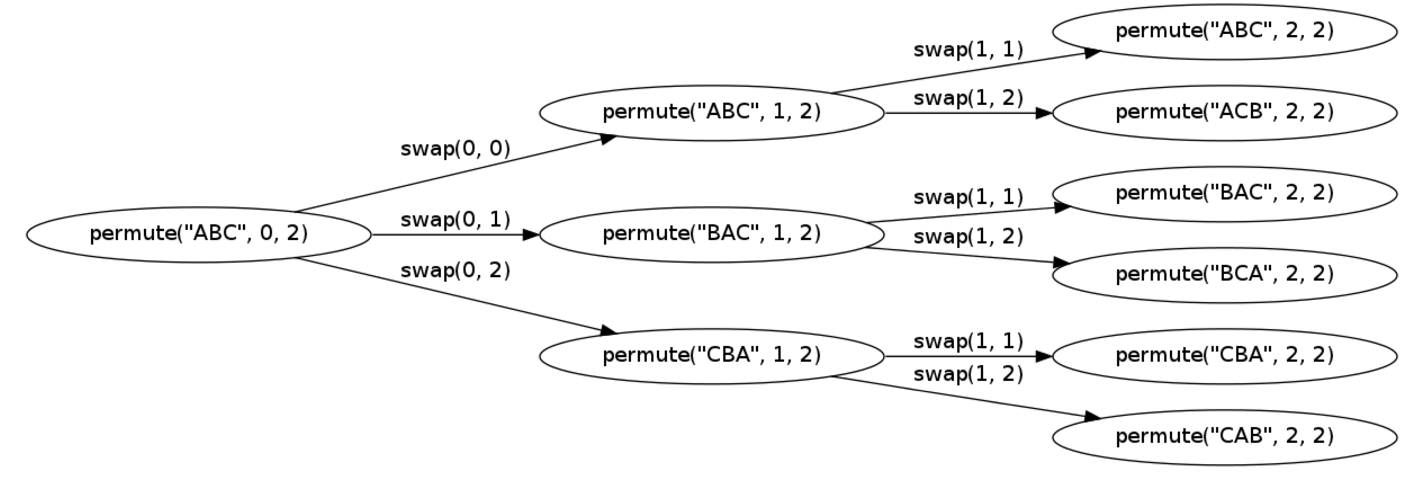
\includegraphics[scale=0.25]{pics/permutation.png}
\end{center}


\begin{lstlisting}[frame=single, language=c++]
void permute(char a[], int i, int n){
	int j;
	if (i == n)
	cout << a << endl;
	else   {
		for (j = i; j <= n; j++)       {
			swap(a[i], a[j]);          
			permute(a, i+1, n);
			swap(a[i], a[j]);
		}
	}
} 		
\end{lstlisting}

	\par compared with subset code, You will find that they are all recursive. permutation is n!
\begin{lstlisting}
permute(i)
for(j...)  //calculate j times same size(i+1) sub problem.
permute(i+1)  //similar with n*f(n-1)		
\end{lstlisting}


\section{Sort}


\subsection{Kth element}

	\par There is a few options to implement Kth element:
	\begin{itemize}
		\item n*log(n) sort
		\item n*k partial select
		\item n*log(k) heap 
		\item quick select, average O(n)
	\end{itemize}

\par k small number, use maxium heap(default)
\begin{lstlisting}
std::priority_queue<int> pq;
for(auto e: arr){
	if(pq.size()<3){
		pq.push(e);
	}
	else if(pq.top()>e){
		pq.push(e);
		pq.pop();
	}
}

while(pq.size()>0){
	cout<<pq.top()<<endl;
	pq.pop();
}		
\end{lstlisting}

	\par Basic idea is \textbf{quick select}, but we use median of median method to get good pivot, to make at the worst 30-70 partition. Pay attention to the k value need to be adjusted when you call a function recursively. 
	
\begin{itemize}
	\item WE should use left close, and right close method to deal with Divide conquer array problem. It will make your code a little easier. 
	
	\item k-1, index is based on 0, but k is based on 1, that is why we need k-1 in line 18
\end{itemize}	
	
\begin{lstlisting}
int partition(vector<int>& arr, int l, int r) {
	int x = arr[r], i = l;
	for (int j = l; j <= r - 1; j++) {
		if (arr[j] <= x) {
			swap(arr[i], arr[j]);
			i++;
		}
	}
	swap(arr[i], arr[r]);
	return i;
}

int quickselect(vector<int>& A, int left, int right, int k){
	//p is position of pivot in the partitioned array
	int p = partition(A, left, right);
	
	//k equals pivot got lucky
	if (p == k-1){
		return A[p];
	}
	//k less than pivot
	else if (k - 1 < p){
		return quickselect(A, left, p - 1, k);
	}
	//k greater than pivot
	else{
		return quickselect(A, p + 1, right, k);
	}
}

vector<int> A = {1,3,8,2,4,9,7};
int k = 5;
cout<<quickselect(A, 0, 6, 5); //output is 7
\end{lstlisting}
	
	\par Stable\_partition. The whole idea is just like merge sort, Pay attention here, merge sort is also stable sort. 
\begin{lstlisting}
#include <algorithm>

template <typename Iterator, typename Predicate>
Iterator my_stable_partition(Iterator first, Iterator last, Predicate predicate) {
	auto n = std::distance(first, last);
	if (n <= 1) {
		if (n == 1 && predicate(*first))
			++first;
		return first;
	}
	auto middle = first;
	std::advance(middle, n / 2);
	auto a = my_stable_partition(first, middle, predicate);
	auto b = my_stable_partition(middle, last, predicate);
	return std::rotate(a, middle, b);
}	
\end{lstlisting}
	
	\par median of medians (advance part, skip it if you don't have enough time.)
\begin{lstlisting}[frame=single, language=c++, basicstyle=\scriptsize]
int array[] = { 1,12,3,4,1,      5,2,7,8,88,      5,2,32,1,35,   -1,7,5,38,-11 };

int insertSort(int left, int right) {
	for (int i = left + 1; i <= right; i++) {
		int temp = array[i], j;
		for (j = i; j > left && array[j - 1] > temp; j--) array[j] = array[j - 1];
		array[j] = temp;
	}
	return (left + right) >> 1;
}

int BFPRT(int, int, int);

int getPivotIndex(int left, int right) {
	if (right - left < 5) return insertSort(left, right);
	int back = left - 1;
	for (int i = left; i + 4 < right; i += 5) {
		std::cout << "i" << i <<" "<< right<<std::endl;
		int index = insertSort(i, i + 4);
		std::swap(array[++back], array[index]);
	}
	return BFPRT(left, back, ((left + back) >> 1) + 1);
}


int partition(int left, int right, int pivotIndex) {
	std::swap(array[right], array[pivotIndex]);
	int mid = left;
	for (int i = left; i < right; i++) {
		if (array[i] < array[right])
		std::swap(array[i], array[mid++]);
	}
	std::swap(array[right], array[mid]);
	return mid;
}

int BFPRT(int left, int right, int k) {
	int pivotIndex = getPivotIndex(left, right);
	int mid = partition(left, right, pivotIndex);
	int count = mid - left + 1;
	if (count == k) {
		return mid;
	}
	else if (count > k) {
		return BFPRT(left, mid - 1, k);
	}
	else {
		return BFPRT(mid + 1, right, k - count);
	}
}

int main() {
	int k = 5;
	int length = sizeof(array) / sizeof(array[0]);
	for (int i = 0; i < length; i++) {
		std::cout << array[i] << "  ";
	}
	std::cout << std::endl << " " << k << " ";
	std::cout << array[BFPRT(0, length - 1, k)] << std::endl;
	return 0;
}
	
\end{lstlisting}


\subsection{Simple sort}

	
	\par All sort algorithm don't compare equal relationship. So some algorithm is Stable, and other is not stable. Bubble is simple source code stable sorting. All the sorting is from minimum to maximum default.

 

	\par for all sort comparsion, there is good ref website: \newline  https://www.toptal.com/developers/sorting-algorithms/selection-sort

	\par Selection sort is an in-place comparison sort. O(n2). The algorithm finds the minimum value, swaps it with the value in the first position.  And repeat From the comparisons presented here, one might conclude that selection sort should never be used. It does not adapt to the data in any way (notice that the four animations above run in lock step), so its runtime is always quadratic. However, selection sort has the property of minimizing the number of swaps. In applications where the cost of swapping items is high, selection sort very well may be the algorithm of choice. Selection sort only need O(n) write, so if write is expensive operation, you need to use it. 
\begin{lstlisting}[frame=single, language=c++]
For(int size=n ;size>1;size--){
	Int j = Max(a,size);
	Swap(a[j],a[size-1]);
}
\end{lstlisting}

	\par Insertion sort is suitable for small list and mostly sorted list. Although it is one of the elementary sorting algorithms with O(n2) worst-case time, insertion sort is the algorithm of choice either when the data is nearly sorted (because it is adaptive) or when the problem size is small (because it has low overhead). For these reasons, and because it is also stable, insertion sort is often used as the recursive base case (when the problem size is small) for higher overhead divide-and-conquer sorting algorithms, such as merge sort or quick sort. Insertion sort is also stable sort. 

\begin{lstlisting}[frame=single, language=c++]
For(int I = 0;i<n;i++){
Int iv = a[i];
Insert(a,I, iv);
}
Insert(a[],int n,int lv){
For(int I = n-1;i>=0&&lv<a[i];i--)
    A[i+1]=a[i]  //move each element from tail to head one by one
A[i]  = lv;  //insert here. 
}
\end{lstlisting}

	\par Bubble sort is stable. Bubble sort can stops after reaching a sorted array. In the best case (already sorted), every insert requires constant time. So Bubble and insert can reach O(n) time in Best context. Bubble sort has many of the same properties as insertion sort, but has slightly higher overhead. In the case of nearly sorted data, bubble sort takes O(n) time, but requires at least 2 passes through the data (whereas insertion sort requires something more like 1 pass).
\begin{lstlisting}[frame=single, language=c++]
For (int I = n;i>0;i--){
	For(int j= 0;j<I;j++)
		If(a[j]<a[j+1]) swap(a[j],a[j+1]);
}
\end{lstlisting}


	\par In insertion sort elements are bubbled into the sorted section, while in bubble sort the maximums are bubbled out of the unsorted section.

\begin{lstlisting}
	//insert sort
	sorted  | unsorted
	1 3 5 8 | 4 6 7 9 2
	1 3 4 5 8 | 6 7 9 2
	
	bubble sort
	unsorted  | biggest
	3 1 5 4 2 | 6 7 8 9
	1 3 4 2 | 5 6 7 8 9
\end{lstlisting}

\par Difference between insertion sort and selection sort? The real question is the speed of comparison vs. copying. The time a selection sort will win is when a comparison is a lot faster than copying. Just for example, let's assume two fields: a single int as a key, and another megabyte of data attached to it. In such a case, comparisons involve only that single int, so it's really fast, but copying involves the entire megabyte, so it's almost certainly quite a bit slower. Since the selection sort does a lot of comparisons, but relatively few copies, this sort of situation will favor it. The insertion sort does a lot more copies, so in a situation like this, the slower copies will slow it down quite a bit.

\par As far as worst case for a insertion sort, it'll be pretty much the opposite -- anything where copying is fast, but comparison is slow. There are a few more cases that favor insertion as well, such as when elements might be slightly scrambled, but each is still within a short distance of its final location when sorted. In another word, insertion sort is more efficient than selection sort when the input array is partially sorted or almost sorted.

\par If the data doesn't provide a solid indication in either direction, chances are pretty decent that insertion sort will work out better.

\subsection{quick sort}

\subsubsection{Quick sort}

	\par Three quick heapSort, MergeSort, quickSort. The time complexity are all (Olog(n)). MergeSort need O(N) extra space, When you merge two lists, this shortcoming can be avoid.

	\par partition 
\begin{lstlisting}[frame=single, language=c++]
/* This function takes last element as pivot, places
   the pivot element at its correct position in sorted
    array, and places all smaller (smaller than pivot)
   to left of pivot and all greater elements to right
   of pivot */
   
partition (arr[], low, high){
    // pivot (Element to be placed at right position)
    pivot = arr[high];   
    i = (low - 1)  // Index of smaller element
    for (j = low; j <= high- 1; j++)    {
        // If current element is smaller than or
        // equal to pivot
        if (arr[j] <= pivot)        {
            i++;    // increment index of smaller element
            swap arr[i] and arr[j]
        }
    }
    swap arr[i + 1] and arr[high])
    return (i + 1)
}
\end{lstlisting}

\begin{center}
	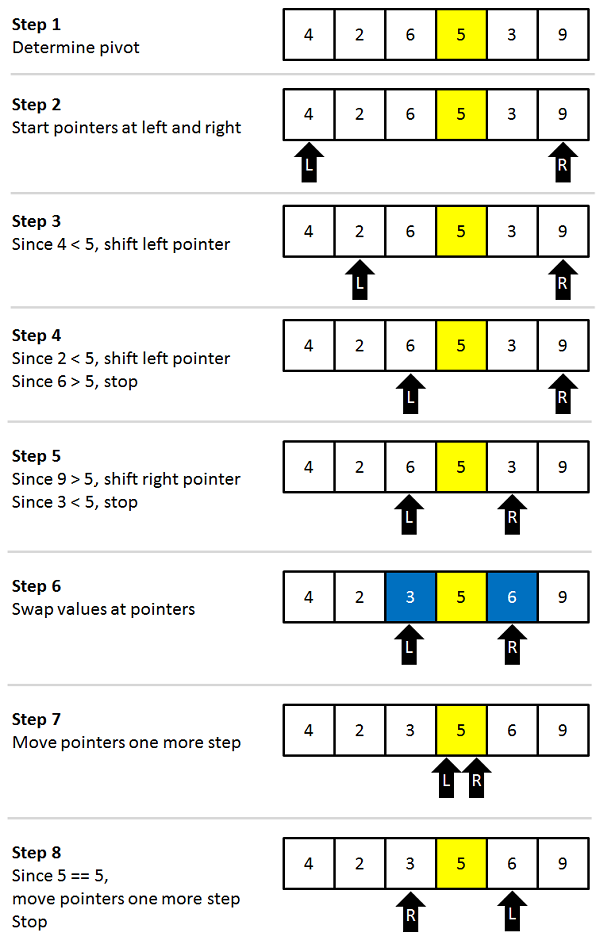
\includegraphics[scale=0.45]{pics/qsort1.png} 
\end{center}

\begin{center}
	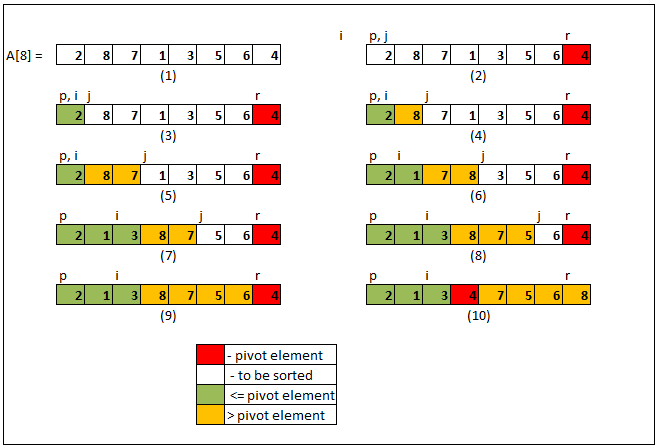
\includegraphics[scale=0.45]{pics/qsort2.png}
\end{center}



\par Quick sort need random access ability.  

\begin{center}
	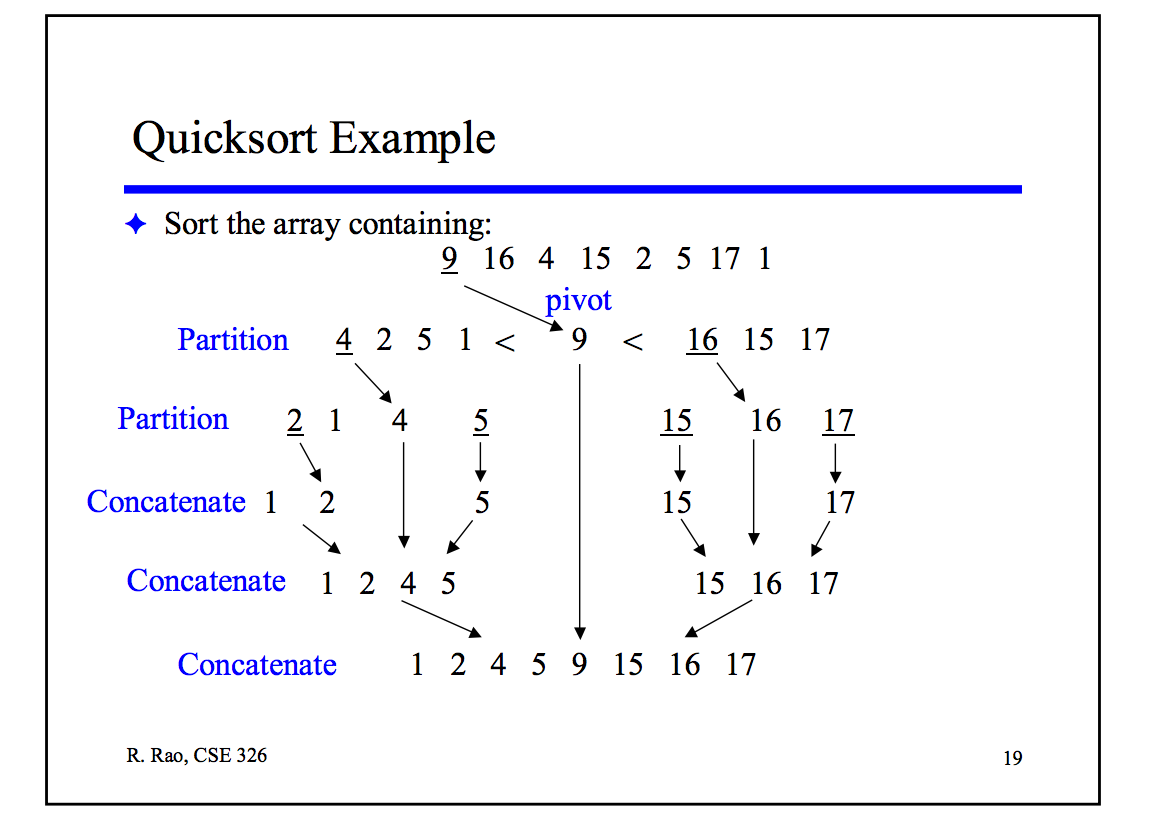
\includegraphics[scale=0.45]{pics/quick_sort.png} 
\end{center}

\begin{center}
	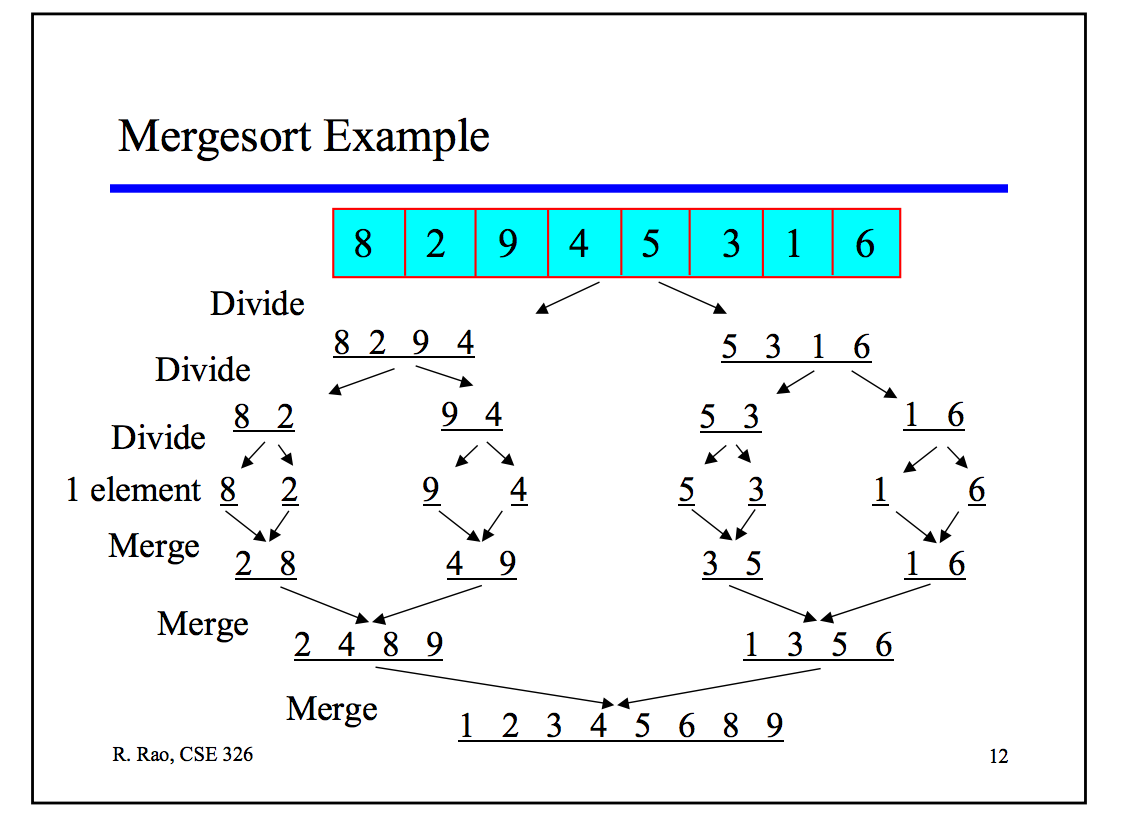
\includegraphics[scale=0.45]{pics/merge_sort.png}
\end{center}




\subsubsection{Merge sort}

	\par Merge sort is often preferred for sorting a linked list. The slow random-access performance of a linked list makes some other algorithms (such as quicksort) perform poorly, and others (such as heapsort) completely impossible. MergeSort(headRef)
	
\begin{verbatim}
	1) If head is NULL or there is only one element in the Linked List 
	then return.
	2) Else divide the linked list into two halves.  
	FrontBackSplit(head, &a, &b); /* a and b are two halves */
	3) Sort the two halves a and b.
	MergeSort(a);
	MergeSort(b);
	4) Merge the sorted a and b (using SortedMerge() discussed here) 
	and update the head pointer using headRef.
	*headRef = SortedMerge(a, b);
\end{verbatim}
\textbf{Idea: 1) No random access 2) recursive}

\begin{lstlisting}[frame=single, language=c++] 
/* sorts the linked list by changing next pointers (not data) */
void MergeSort(struct node** headRef)
{
	struct node* head = *headRef;
	struct node* a, b;
	
	/* Base case -- length 0 or 1 */
	if ((head == NULL) || (head->next == NULL)){
		return;
	}
	
	/* Split head into 'a' and 'b' sublists */
	FrontBackSplit(head, &a, &b); 
	
	/* Recursively sort the sublists */
	MergeSort(&a);
	MergeSort(&b);
	
	/* answer = merge the two sorted lists together */
	*headRef = SortedMerge(a, b);
}		
\end{lstlisting}

\begin{lstlisting}[frame=single, language=c++] 
/* See http://geeksforgeeks.org/?p=3622 for details of this function */
struct node* SortedMerge(struct node* a, struct node* b){
	struct node* result = NULL;	
	/* Base cases */
	if (a == NULL)
	return(b);
	else if (b==NULL)
	return(a);
	
	/* Pick either a or b, and recur */
	if (a->data <= b->data){
		result = a;
		result->next = SortedMerge(a->next, b);
	}
	else{
		result = b;
		result->next = SortedMerge(a, b->next);
	}
	return(result);
}	
\end{lstlisting}
\begin{description}
	\item[Source code:] \textbf{Idea: recursive}
\end{description}

	\par Inplace merge
\begin{lstlisting}
void swapNums(vector<int>&ivNums, int lo, int hi){
	--hi;
	while (lo<hi)
	{
		swap(ivNums[lo++], ivNums[hi--]);
	}
}

void MergeInPlace(vector<int>&ivNums, int lo, int mid, int hi){
	int i = lo, j = mid;
	while (j<hi)//stop when the latter half is empty
	{
		while (i < j&&ivNums[i] <= ivNums[j])
		{
			++i;
		}
		while (j<hi&&ivNums[i] > ivNums[j])
		{
			++j;
		}
		//just std::rotate
		swapNums(ivNums, i, j);
		swapNums(ivNums, i, i + j - mid);
		swapNums(ivNums, i + j - mid, j);
		
		//reset the boundary and continue.
		i = i + j - mid;
		mid = j;
	}
}
\end{lstlisting}

\begin{center}
	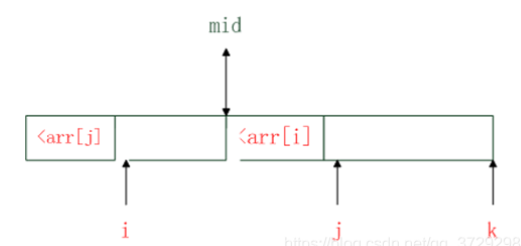
\includegraphics[scale=0.45]{pics/inplace}
\end{center}

\subsubsection{heap sort}

\par The most import thing is heapify, 0then push the maxium element to the 0 index, then swap to the last position, then heapify the (0, len-1), then (0, len-2)....
\begin{lstlisting}
// To heapify a subtree rooted with node i which is
// an index in arr[]. n is size of heap
void heapify(int arr[], int n, int i)
{
	int largest = i; // Initialize largest as root Since we are using 0 based indexing
	int l = 2 * i + 1; // left = 2*i + 1
	int r = 2 * i + 2; // right = 2*i + 2
	
	// If left child is larger than root
	if (l < n && arr[l] > arr[largest])
	largest = l;
	
	// If right child is larger than largest so far
	if (r < n && arr[r] > arr[largest])
	largest = r;
	
	// If largest is not root
	if (largest != i) {
		swap(arr[i], arr[largest]);
		
		// Recursively heapify the affected sub-tree
		heapify(arr, n, largest);
	}
}

// main function to do heap sort
void heapSort(int arr[], int n)
{
	// Build heap (rearrange array)
	for (int i = n / 2 - 1; i >= 0; i--)
	heapify(arr, n, i);
	
	// One by one extract an element from heap
	for (int i = n - 1; i >= 0; i--) {
		// Move current root to end
		swap(arr[0], arr[i]);
		
		// call max heapify on the reduced heap
		heapify(arr, i, 0);
	}
}

\end{lstlisting}



\subsubsection{introsort}

\par This is the method used in STL.

\begin{lstlisting}[frame=single, language=c++]
// A Utility function to perform intro sort
void IntrosortUtil(int arr[], int * begin, int * end, int depthLimit){
	// Count the number of elements
	int size = end - begin;
	
	// If partition size is low then do insertion sort
	if (size < 16){
		InsertionSort(arr, begin, end);
		return;
	}
	
	// If the depth is zero use heapsort
	if (depthLimit == 0){
		make_heap(begin, end+1);
		sort_heap(begin, end+1);
		return;
	}
	
	// Else use a median-of-three concept to
	// find a good pivot
	int * pivot = MedianOfThree(begin, begin+size/2, end);
	
	// Swap the values pointed by the two pointers
	swapValue(pivot, end);
	
	// Perform Quick Sort
	int * partitionPoint = Partition(arr, begin-arr, end-arr);
	IntrosortUtil(arr, begin, partitionPoint-1, depthLimit - 1);
	IntrosortUtil(arr, partitionPoint + 1, end, depthLimit - 1);
	
	return;
}	
\end{lstlisting}	


\subsection{Bucket and radix sort}


\par Bucket sort is not comparison algorithm.  we must know the maximum value in the unsorted array and how many objects in the unsorted array. If maximum value is not big, and objects is a lot. such as all student score (<100) in a country(1000000). At this time, we can use Bucket sort. 
	
\par Firstly, we must know how to handle duplicates. Secondly,  Thirdly, we must have enough memory. If you sort telephone which will not allow duplicated value, you can build an bit array. And set bit 1 if there are number exist. It will save a lot of memories.   For duplicate, you can store a link in each bucket. (array item)

\par Radix sort is cousin of Bucksort. BucketSort is more efficient for 'Dense' arrays, while RadixSort can handle sparse (well, not exactly sparse, but spaced-out) arrays well. Use \% operator to get radix each digit. 

\par $ 1\sim n^c-1$, such as $ 1\sim10^3-1 $  You can use 10 as radix, and sort it 3 times. 

\subsubsection{Bucket sort}
	
	\par Basic step:  Here, Link list is best option to implement a bucket. Because Nobody will now how many elements will be put into the each bucket. 
	\begin{enumerate}
		\item Set up an array of initially empty "buckets".
		\item Scatter: Go over the original array, putting each object in its bucket. 
		\item Sort each non-empty bucket.(Optional )
		\item Gather: Visit the buckets in order and put all elements back into the original array.
	\end{enumerate}
	


\subsubsection{Radix sort}


	\par r is radix, $x\%r, (x\%r^{2})/r, (x\%r^{3})/r^{2}$  get each digit from least significant digit (LSD) radix sorts to most significant digit. 
	
\begin{lstlisting}[frame=single, language=c++]
int i ;
int k;
while(i%10){
	k = i%10;
	i = i/10;
}	
\end{lstlisting}	
	
	\begin{enumerate}
		\item according to r, prepare two arrays buckets A, B. 
		\item Sort according to one position and put them into A array buckets. 
		\item loop through A array buckets, and get next position digit. and then according to its value put into B array buckets.
		\item swap A,B two array, then goto step 2.
	\end{enumerate}
	
	\par Difference between radix sort and quick sort. Quicksort/Introsort is more flexible:Quicksort and Introsort work well with all kinds of data. All you need for sorting is the possibility to compare items. This is trivial with numbers but you can sort other data as well. Radix sort on the other hand just sorts things by their binary representation. It never compares items against each other. Radix sort needs more memory. All radix sort implementations that I've seen use a secondary buffer to store partial sorting results. This increases the memory requirements of the sorting algorithm. That may not be a problem if you only sort a couple of kilobytes, but if you go into the gigabyte range it makes a huge difference. If I remember right a in place radix-sort algorithm exist on paper though.
	
\begin{lstlisting}
void countSort(int arr[], int n, int exp){
	
	int output[n];  // Output array
	int i, count[10] = { 0 };
	
	// Store count of occurrences in count[]
	for (i = 0; i < n; i++)
	count[(arr[i] / exp) % 10]++;
	
	// Change count[i] so that count[i] now contains actual position
	// of this digit in output[]
	for (i = 1; i < 10; i++)
	count[i] += count[i - 1];
	
	// Build the output array
	for (i = n - 1; i >= 0; i--) {
		output[count[(arr[i] / exp) % 10] - 1] = arr[i];
		count[(arr[i] / exp) % 10]--;
	}
	
	// Copy the output array to arr[], so that arr[] now contains sorted
	// numbers according to current digit
	for (i = 0; i < n; i++)
	arr[i] = output[i];
}

// The main function to that sorts arr[] of size n using Radix Sort
void radixsort(int arr[], int n){
	
	// Find the maximum number to know number of digits
	int m = getMax(arr, n);
	
	// Do counting sort for every digit. Note that instead of passing digit
	// number, exp is passed. exp is 10^i where i is current digit number
	for (int exp = 1; m / exp > 0; exp *= 10)
		countSort(arr, n, exp);
}	
\end{lstlisting}	
	
	\par In order to understand previous code, you need to understand counting sort, Detail can be found here: //
	
	https://www.geeksforgeeks.org/counting-sort/
	//
	it use prefix sum(std::partial\_sum). it's also interesting application of std::partial\_sum, you need to remember it. 

\subsection{Summary}
\par You can compare sorting algorithms against the following criteria:
\begin{itemize}
	\item Time Complexity (Big-O notation). You should note that best-case, worst-case and average run-time can have different time complexity. For example best-case for Bubble Sort is only O(n), making it faster than Selection Sort when the original list is mostly in order (not many elements out of place).
	\item Memory Complexity. How much more memory is required to sort a list as n grows?
	
	\item Stability. Does the sort preserve the relative ordering of elements that have equivalent sort values? (For example if you were sorting a list of catalog items by their price, some elements may have equal prices. If the catalog was originally sorted alphabetically by item name, will the chosen sort algortihm preserve the alphabetical ordering within each group of equal-priced items.)
	
	\item Best/Worst/Averavge number of comparisons required. Important when compare operations are expensive. (For example: comparing efficiencies of alternative designs where efficiency is calculated via some simulation or otherwise complex calculation).
	
	\item Best/Worst/Average number of swap operations required. Important when swap operations are expensive. (For example: sorting shipping containers that must be physically moved on the deck of a ship)
	
	\item Code size. Bubble-sort is known for its small code footprint.
\end{itemize}


\section{Greedy}

\par Idea of Greedy:
\begin{itemize}
\item Solve a problem by making a sequence of decisions.

\item Decisions are made one by one in some order.

\item Each decision is made using a greedy criterion. At each stage we make a decision that appears to be the best at the time.

\item A decision, once made, is (usually) not changed later. 
\end{itemize}


\par	You need a \textbf{greedy criterion} to make a local decision. For examples: making change, 0/1 knappack,  activity selection (largest subset) sorted according to their finishing time, topological orders. Dijkstra, Kruskal, prim and collin.

\par Applications: Container Loading, 0/1 knapsack problem, Topological sorting, Bipartite cover, Single-source shortest paths, Minimum-cost spanning trees. 


\subsubsection{Intervals questions}

	\par \textbf{two basic tricks, sort, then do something when it overlap}.


	\par Meeting room questions. 
	\begin{enumerate}
		\item Minimum empty time. That is 0/1 knapback problem.
		\item Two group collision intervals.
	\end{enumerate}
	

	\par Overlap (three questions):
	
\begin{enumerate}
	\item Non-overlap number. one meeting room, maximum meeting number. Sort by end time, delete(ignore) if overlap. 
\begin{lstlisting}
public int intervalSchedule(int[][] intvs) {
	if (intvs.length == 0) return 0;
	// sort
	Arrays.sort(intvs, new Comparator<int[]>() {
		public int compare(int[] a, int[] b) {
			return a[1] - b[1];
		}
	});
	
	int count = 1;
	int x_end = intvs[0][1];
	for (int[] interval : intvs) {
		int start = interval[0];
		if (start >= x_end) {
			// find next non-overlap interval, 
			//update x_end. 
			count++;
			x_end = interval[1];
		}
	}
	return count;
}	
\end{lstlisting}
	
	
	\item Maximum overlap number. Minimum meeting room numbers. sort by start time. you can use scan line.  
\begin{itemize}
	\item Sort the intervals by their start times.
	
	\item Use a min-heap to keep track of the end times of meetings currently using a room.
	
	\item Iterate through the sorted intervals and for each interval:
	
	\begin{enumerate}
		\item If the room due to free up the earliest is free, remove it from the heap.
		
		\item Add the current meeting's end time to the heap.
		
		\item The size of the heap at any point will give the number of rooms required at that time.	
	\end{enumerate}
\end{itemize}

\begin{lstlisting}
// Function to find the minimum number of meeting rooms required
int minMeetingRooms(vector<vector<int>>& intervals) {
	if (intervals.empty()) return 0;
	
	// Sort the intervals by start time
	sort(intervals.begin(), intervals.end(), [](const vector<int>& a, const vector<int>& b) {
		return a[0] < b[0];
	});
	
	// Min-heap to keep track of end times
	priority_queue<int, vector<int>, greater<int>> minHeap;
	
	// Add the end time of the first meeting
	minHeap.push(intervals[0][1]);
	
	for (int i = 1; i < intervals.size(); ++i) {
		// If the room due to free up the earliest is free, remove it from the heap
		if (intervals[i][0] >= minHeap.top()) {
			minHeap.pop();
		}
		// Add the current meeting's end time to the heap
		minHeap.push(intervals[i][1]);
	}
	
	// The size of the heap is the number of rooms required
	return minHeap.size();
}

int main() {
	vector<vector<int>> intervals = {{5, 10}, {0, 30}, {15, 20}};
	cout << "Minimum number of meeting rooms required: " << minMeetingRooms(intervals) << endl;
	return 0;
}
\end{lstlisting}
	
	
	\item Merge overlap. sort by left. If overlap, then update right point; if non-overlap, find a new current intervals. 

\begin{lstlisting}
vector<vector<int>> mergeOverlap(vector<vector<int>>& arr) {
	
	// Sort intervals based on start values
	sort(arr.begin(), arr.end());
	
	vector<vector<int>> res;
	res.push_back(arr[0]);
	
	for (int i = 1; i < arr.size(); i++) {
		vector<int>& last = res.back();
		vector<int>& curr = arr[i];
		
		// If current interval overlaps with the last merged
		// interval, merge them 
		if (curr[0] <= last[1]) 
		last[1] = max(last[1], curr[1]);
		else 
		res.push_back(curr);
	}
	
	return res;
}

int main() {
	vector<vector<int>> arr = {{7, 8}, {1, 5}, {2, 4}, {4, 6}};
	vector<vector<int>> res = mergeOverlap(arr);
	
	for (vector<int>& interval: res) 
	cout << interval[0] << " " << interval[1] << endl;
	
	return 0;
}
\end{lstlisting}

\end{enumerate}
	
	\par Interval cover. (two questions)
\begin{enumerate}

	\item Minimum cover

\begin{lstlisting}
int videoStitching(int[][] clips, int T) {
	if (T == 0) return 0;
	// Sort in ascending order by the start point, and in descending order if the start points are the same.
	Arrays.sort(clips, (a, b) -> {
		if (a[0] == b[0]) {
			return b[1] - a[1];
		}
		return a[0] - b[0];
	});
	// Keep track of the number of selected short videos
	int res = 0;
	
	int curEnd = 0, nextEnd = 0;
	int i = 0, n = clips.length;
	while (i < n && clips[i][0] <= curEnd) {
		// Greedily select the next video within the interval of the res-th video.
		while (i < n && clips[i][0] <= curEnd) {
			nextEnd = Math.max(nextEnd, clips[i][1]);
			i++;
		}
		// Find the next video and update curEnd.
		res++;
		curEnd = nextEnd;
		if (curEnd >= T) {
			// The interval [0, T] can already be assembled.
			return res;
		}
	}
	// Unable to continuously assemble the interval [0, T].
	return -1;
}	
\end{lstlisting}

	\item Erase cover. Once find overlap, update right,  find non-overlap, update left and right. 

\begin{lstlisting}
int removeCoveredIntervals(int[][] intvs) {
	// Sort in ascending order by the start point, and in descending order if the start points are the same.
	Arrays.sort(intvs, (a, b) -> {
		if (a[0] == b[0]) {
			return b[1] - a[1];
		}
		return a[0] - b[0]; 
	});
	
	// Record the start and end points of the merged intervals.
	int left = intvs[0][0];
	int right = intvs[0][1];
	
	int res = 0;
	for (int i = 1; i < intvs.length; i++) {
		int[] intv = intvs[i];
		// Case 1: Find the covering intervals.
		if (left <= intv[0] && right >= intv[1]) {
			res++;
		}
		// Case 2: Find the overlapping intervals and merge them.
		if (right >= intv[0] && right <= intv[1]) {
			right = intv[1];
		}
		// Case 3: Completely non-overlapping, update the start and end points.
		if (right < intv[0]) {
			left = intv[0];
			right = intv[1];
		}
	}
	
	return intvs.length - res;
}	
\end{lstlisting} 
	
\end{enumerate}	
	


\subsection{Application}


\par  Machine Scheduling, \textbf{sort all task according to start time, and minheap of machine end time. }

\par Container Loading and 0/1 knapsack problem are different. For 0/1 knapsack problem, we consider the value and weight together,  For greed algorithm, it change time complexity from $2^{n}$to $n.log(n)$, but 583/600 is withing 10\%, so it's very practical algorithm.  Don't underestimate it. 

\par Topological sorting: 
\begin{verbatim}
1) Select any one among vertices having no incoming edge
2) Put the node into the solution &  Remove the node and its outgoing edges from the graph
4) Repeat the above steps until no nodes remain

You need to InDegree[n] array to save and update all the vetex InDegree, and stack to store all the vetex which indegree is 0.  
\end{verbatim}


\par Bipartite-cover problems are NP-hard
\begin{verbatim}
A greedy method to develop a fast heuristic
Construct the cover A’ in stages
Select a vertex of A  using the greedy criterion:
Select a vertex of A that covers the largest # of uncovered vertices of B
\end{verbatim}

\par Dijkstra algorithm.  
\begin{center}
	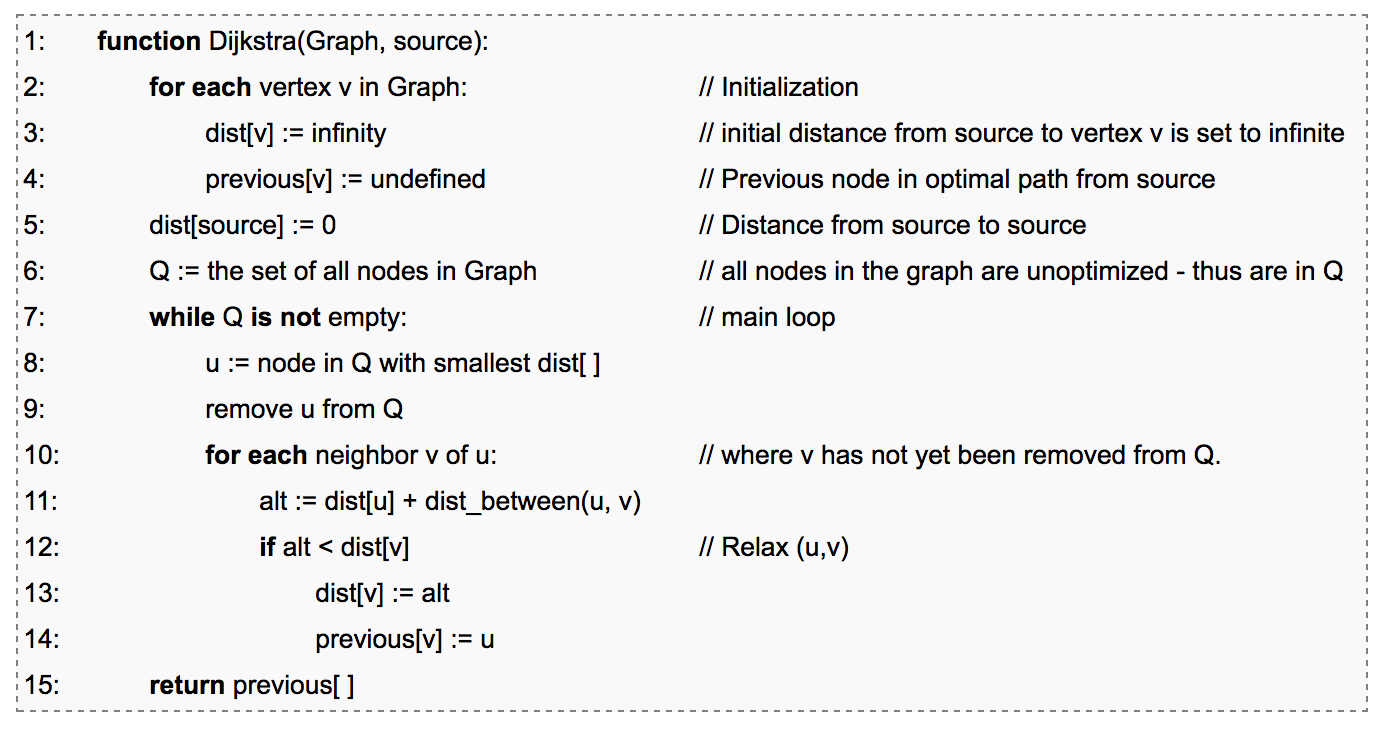
\includegraphics[scale=0.45]{pics/Dijkstra.png} 
\end{center}

\begin{itemize}
\item The greedy idea lies in line 8
\item In line 8, it must shortest path to this vetex,  Because if it's not, There is shorter path, then, according to we select min in line 8, shorter one will be selected first, and this value HAS BEEN updated before. 
\item $O(n^{2})$
\item the shortest value is saved, it's also idea of dynamic programming.
\item Just like vertabi, you can think that they are the same. 
\end{itemize}


\section{Divide Conquer}
\subsection{Binary search}

	\par A binary search (or divide-and-conquer) idea can be applied to the problem of finding the closest pair of points on a plane. By utilizing a subproblem, you can prune some candidate points. Another application is using merge sort to count the number of smaller elements to the right of each element, which is introduced by labuladong. The fundamental idea is still binary search, but the specifics come from the fact that merge sort maintains order, and this characteristic can be used to count the number of smaller elements on the right. This is a rather unique application.
	
	\par The key idea here is leveraging the sorting order inherent in merge sort to solve a problem related to counting elements, and it also shows the pruning advantage in divide-and-conquer algorithms.
	
	\par Binary search

\begin{lstlisting}[frame=single, language=c++]
int binarySearch(int arr[],int target, int i, int j) {
	int left = i;
	int right = j;
	while ( left<= right) {
		int mid = (left+right)/2;
		if (arr[mid] > target)
			right = mid - 1;
		else if (arr[mid] < target)
			left = mid + 1;
		else if (arr[mid] == target)
			return mid;
	}
	return -1;
} 
\end{lstlisting}

\begin{lstlisting}[frame=single, language=c++]
int left_bound(int arr[],int target, int i, int j) {
	int left = i;
	int right = j;
	while ( left<= right) {
		int mid = (left+right)/2;
		if (arr[mid] > target)
			right = mid - 1;
		else if (arr[mid] < target)
			left = mid + 1;
		else if (arr[mid] == target)
			right = mid-1;  //1) reduce to right in order to find left bound
	}
	
	if (left > j || arr[left] != target)
		return -1;  //3) in order to return left, left will go to the right boundary, 
	return left; //2) return left.   
}
\end{lstlisting}	


\begin{lstlisting}[frame=single, language=c++]
int right_bound(int arr[],int target, int i, int j) {
	int left = i;
	int right = j;
	while ( left<= right) {
		int mid = (left+right)/2;
		if (arr[mid] > target)
			right = mid - 1;
		else if (arr[mid] < target)
			left = mid + 1;
		else if (arr[mid] == target)
			left = mid+1;  //1) step left to find right bound
	}
	
	if (right < 0 || arr[right] != target)
		return -1;  //3) in order to return right, right will be too small
	return right; //2) return right.   
}	
\end{lstlisting}
	
	\par Three methods summary are below:
\begin{itemize}
	\item close left and right
	\item left bound reduce right, right bount add left;
	\item left bound return left, right bound return right.
	\item left may be too big, right maybe too small. 
	\item if no found, 
\begin{lstlisting}[frame=single, language=c++]
//if we want to find 4, then right point to 3, left point to 5
//when we quit while loop. 
//so left_bount return the 5 (smallest bigger than target),  
//right bount return 3( biggest smaller than target.)
right left
  3    5
\end{lstlisting}	


\begin{center}
		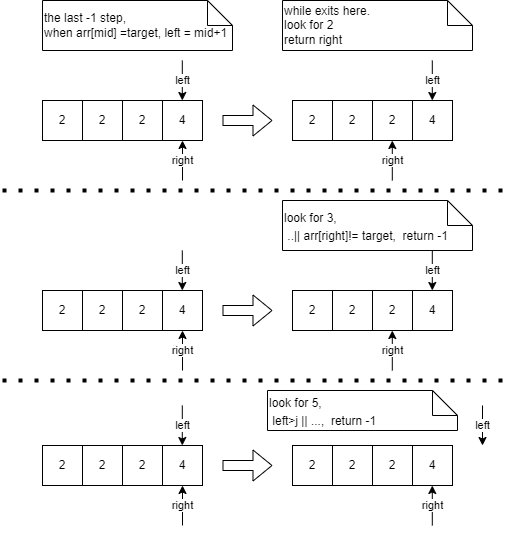
\includegraphics[width=0.7\linewidth]{pics/binary_search.drawio.png}
\end{center}

\end{itemize}

	\par Right boundary logic can be used to found square root. 
\begin{lstlisting}
int mySqrt(int x) {
	int l = 0;
	int r = x/2;
	while(l<=r){
		int mid = l + (r-l)/2;
		int temp = mid*mid;
		if(temp<x){
			l = mid+1;
		}
		else if(temp>x){
			r = mid-1;
		}
		else if(temp == x){
			r = mid;
			break;
		}
	}
	return r; //round down value, for 8, result is 2
	return l; //round up value, for 8, result is 3
}
------
l
2 3    // (l+r)/2 is till l
  r   
------
  l
2 3   //so ++l, 
  r
------
  l
2 3   //mid>x, so --r; l<r, while end.
r     //at this time l points 3, r points 2.
\end{lstlisting}

\subsection{Other }

%\item binary search:
%\begin{enumerate}
%\item only compare once, just  
%\item avoid s+e overflow.
%\item s will catch up e in the end, then break while loop 
%\item check a[m] == k outside of while
%\end{enumerate}
%
%\begin{lstlisting}[frame=single, language=c++]
%while(s<e) {
%    //m=(s+e)/2;
%    m = s/2+e/2 + s&e&1;
%    if(a[m]<k)
%        s = m+1;
%    else 
%       e = m;
%}
%if(a[m] == k) 
%       return ture; 
%\end{lstlisting}


	\par An element in a sorted array can be found in O(log n) time via binary search. But suppose we rotate an ascending order sorted array at some pivot unknown to you beforehand. So for instance, 1 2 3 4 5 might become 3 4 5 1 2. Devise a way to find an element in the rotated array in O(log n) time.

The basic idea is DC(divided conquer.) 
\begin{enumerate}
	\item Use DC, The first part is end condition. For this question, the end atomic condition is e-b == 1(only two elements in it)
	\item If use array, better use index directly.
	\item When you have last atomic condition, you need to decide boundary  b, (e-b)/2, e. \textbf{When you decide boundary , you have to make half part of contents still includes answer. That is very useful hint for you to decide boundary value}
\end{enumerate}

\begin{lstlisting}[breaklines]
size_t find_rot(const vector<int> &vi, int b, int e){
	if (e-b ==1){
		return b;		
	}
	int pivot = b + (e-b)/2;
	cout<<"pivot"<<pivot<<endl;
	if (vi[b]<vi[pivot]){ 
		return find_rot(vi, pivot, e);
	}
	else{
		return find_rot(vi, b, pivot);
	}
}	
\end{lstlisting}
\begin{description}
	\item[label] \textbf{If you can divide it according certain condition, then you can use DC}
\end{description}



\section{Backtracking}
\subsection{Basic}

	Backtracking is particularly useful for solving problems where you need to explore all possible solutions, but you can prune certain paths that are unlikely to lead to a valid solution (i.e., "backtrack" when a partial solution cannot be completed). Problems suitable for backtracking typically involve making a sequence of decisions and can be described as "constraint satisfaction" problems.

\par Here are common types of questions suitable for backtracking:

\begin{itemize}
	\item Combinatorial Problems
Permutations and Combinations: Finding all permutations or combinations of a set of numbers or characters.
Example: Generate all permutations of a given array of numbers.
Subsets: Generating all subsets of a set.
Example: Finding all subsets of a given set of numbers (power set).

	\item  Constraint Satisfaction Problems (CSPs)
Sudoku Solver: Filling in numbers on a Sudoku board while satisfying the row, column, and grid constraints.
N-Queens Problem: Placing N queens on an N×N chessboard so that no two queens attack each other.
Crossword Puzzle Filler: Filling a crossword grid while ensuring valid word placements.

	\item Graph and Tree Search Problems
Maze Solver: Finding a path from start to finish in a maze.
Hamiltonian Path/Cycle: Finding a path or cycle in a graph that visits every vertex exactly once.
Word Search: Searching for words in a grid of characters by moving horizontally, vertically, or diagonally.

	\item  Partitioning Problems
Partition to K Equal Sum Subsets: Partitioning an array into K subsets such that the sum of elements in each subset is equal.
Palindrome Partitioning: Partitioning a string into substrings, where each substring is a palindrome.

	\item  Combinatorial Optimization Problems
Knapsack Problem: Finding combinations of items that maximize value without exceeding the capacity of a knapsack (although dynamic programming is often more efficient for this problem).
Job Scheduling: Scheduling jobs on a limited number of resources (machines) without conflicts.

	\item String Matching
Regular Expression Matching: Checking if a string matches a given pattern with wildcard characters.

	\item  Puzzle Solving
Crossword or Word Puzzle: Solving word puzzles by filling blanks with valid words from a dictionary.
Solving Puzzles like the 8-Puzzle: Rearranging pieces on a grid to reach a specific target configuration.

\end{itemize}

\par In all these cases, backtracking explores the possible decisions recursively but abandons a path (backtracks) if it becomes clear that it cannot yield a valid solution, thus reducing unnecessary computation.

	
	\par The basic backtracking code
\begin{lstlisting}[frame=single, language=c++]
result = []
def backtrack(track, select_list):
	if end_condition:
		result.add( track)
		return

	for option in select_list:
		select one
		backtrack(track, select_list)
		revert the select	
\end{lstlisting}

	\par below is DFS. There is two different: 1) In DFS, we don't need to records all the path, so just don't use track. 2) DFS need to check if unvisited. but most backtrack problem deal with multi-branch tree problem(such as permutation or eight queen problem), so usually we don't check if node is unvisited. The basic idea is the same. 
\begin{lstlisting}[frame=single, language=c++]
DFS(current){
	visit current;
	for all(next to current){
		if(unvisited(next)){
			DFS(next);
		}
	}
}	
\end{lstlisting} 

	\par If we don't want to return all the result, but one, we can change it to below code. 
\begin{lstlisting}[frame=single, language=c++]
result = []
bool backtrack(track, select_list):
	if end_condition:
		result.add(track)
		return true;
	
	for option in select_list:
		select one
		if(backtrack(track, select_list))
			return true;
		revert the select	
\end{lstlisting}
\begin{description}
	\item[Line9-10] This if will stop the recursive and return the true direct to the root.
\end{description}

	\par If we want to remember all the result, we need to List<List>. List inside remember a track, List outside remember all the valid resule. 

\begin{lstlisting}
List<List<Integer>> res = new LinkedList<>();
 //remember recursive path
LinkedList<Integer> track = new LinkedList<>();

public List<List<Integer>> subsets(int[] nums) { // main function
	backtrack(nums, 0);
	return res;
}


void backtrack(int[] nums, int start) {
	res.add(new LinkedList<>(track));
	for (int i = start; i < nums.length; i++) { // main frame
		track.addLast(nums[i]); // select
		backtrack(nums, i + 1); //  use start to trim
		track.removeLast(); // unselect
	}
}


\end{lstlisting}


\subsection{permutation, combination and subset}
\subsubsection{no duplicate, single select}

	\par Two important tree structures.
\begin{center}
	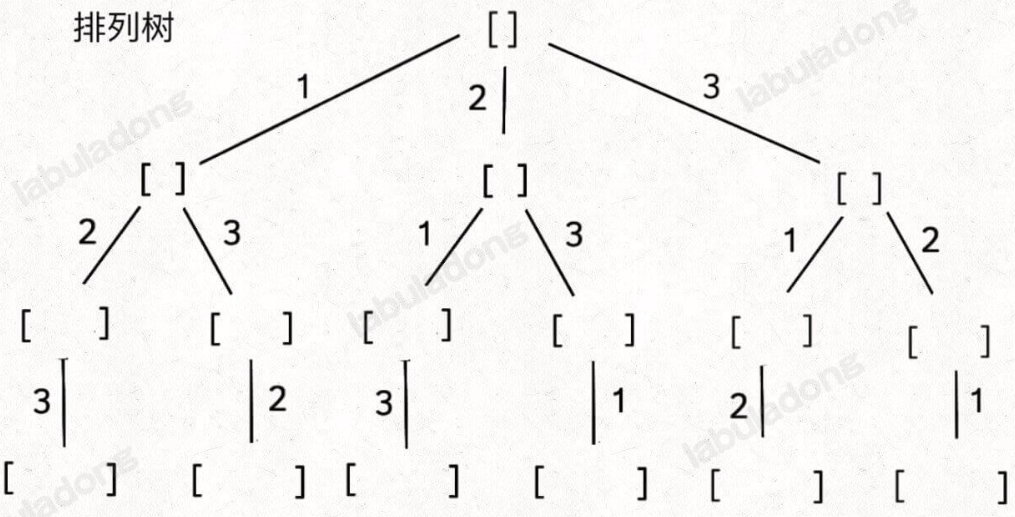
\includegraphics[width=0.5\linewidth]{pics/per}
\end{center}

\par Combination can be seen as a child question of subset.  permutation n!,  subset is $2^n$,  combination is c(n, k). six elements.  5! = 120,  $2^5$ = 32.  c(5, 2) = 10. 

\begin{minipage}{.5\textwidth}		
	\begin{center}
		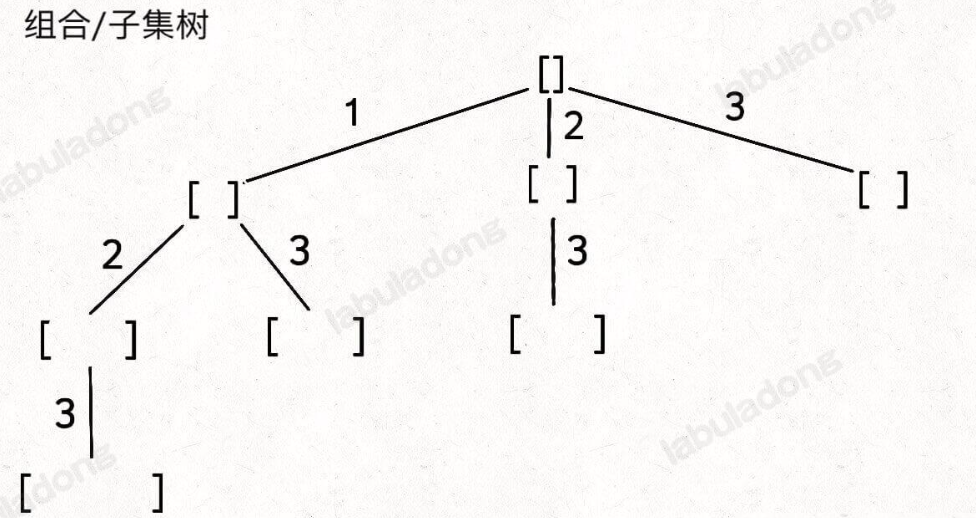
\includegraphics[width=0.8\linewidth]{pics/com} 
	\end{center}
\end{minipage}	
\begin{minipage}{.5\textwidth}		
	\begin{center}
		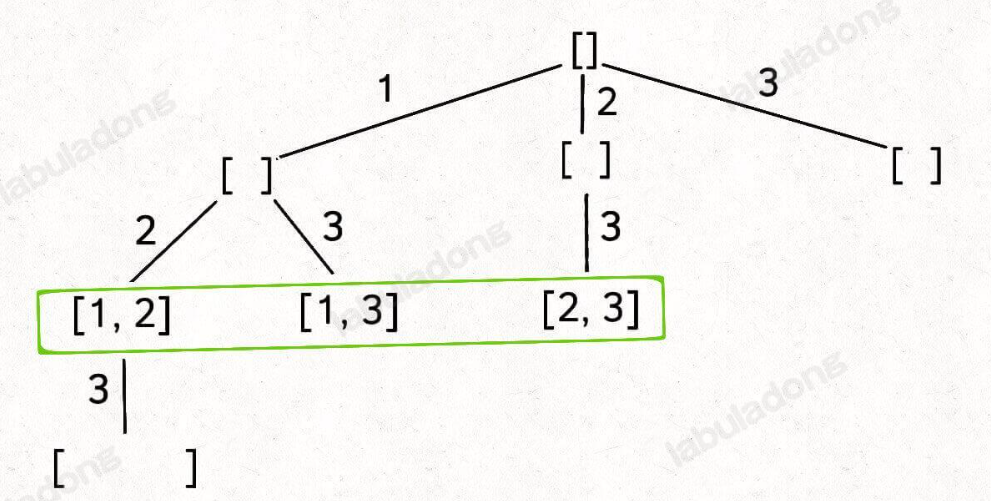
\includegraphics[width=0.8\linewidth]{pics/subset}
	\end{center}
\end{minipage}

	\par \textbf{Subset problem}. 
\begin{enumerate}
	\item Each node(from current node to root,including root(empty set)) is an answer
	\item Don't need base case here.  when i>=len, for will return without any execution.
	\item Refer the combination tree figure to help to understand this code
\end{enumerate}
	
\begin{lstlisting}
void sub(int arr[], int len, int start, vector<int>& result) {
	cout << "one answer is ( ";
	for (int i = 0; i < result.size(); i++) {
		cout << result[i] << " ";
	}
	cout << ")" << endl;
	
	for (int i = start; i < len; ++i) {
		result.push_back(arr[i]);  
		sub(arr, len, i + 1, result);
		result.pop_back();
	}
}

sub(arr, 3, 0, result)
\end{lstlisting}
	
	\par \textbf{Combination problem}, the same idea as subset, just add a parameter k. When one answer length is k, print it out. 
	
\begin{lstlisting}
void com(int arr[], int len, int start, int k, vector<int>& result){
	if (result.size() == k) {
		cout << "one answer is ( ";
		for (int i = 0; i < result.size(); i++) {
			cout << result[i] << " ";
		}
		cout << ")" << endl;
	}
	
	for (int i = start; i < len; ++i) {
		result.push_back(arr[i]);  
		com(arr, len, i + 1, k, result);
		result.pop_back();
	}
}	
\end{lstlisting}

	\par \textbf{Permutation problem}. 
	
\begin{itemize}
	\item Base case is size == len
	\item You must use used array here to remember which element you have used. 
\end{itemize}
\begin{lstlisting}
void per(int arr[], int len, int used[], vector<int>& result) {
	if (result.size() == len) {
		cout << "one answer is ( ";
		for (int i = 0; i < result.size(); i++) {
			cout << result[i] << " ";
		}
		cout << ")" << endl;
	}
	for (int i = 0; i < len; ++i) {
		if (used[i] == 1)
			continue;
		result.push_back(arr[i]); 
		used[i] = 1;
		per(arr, len, used, result);
		result.pop_back();
		used[i] = 0;
	}
}	
\end{lstlisting}
	\par For permutation problem, there is another easy implementation. You don't need extra result vector, but you have to use swap. They use the same basic backtrack idea.
\begin{lstlisting}
//all permutation. here there is a trick, we don't need track, but the basic idea is the same. 
void permute(char a[], int i, int n){
	int j;
	if (i == n){  //end_condition, 
		cout << a << endl;
		return;
	}
	
	for (j = i; j <= n; j++){  // all options in select_list
		swap(a[i], a[j]);     //select one
		permute(a, i+1, n);
		swap(a[i], a[j]);    //revoke select.
	}
} 	
\end{lstlisting}



\subsubsection{No duplicate, multi select}

	\par The basic idea is just like before, for combination, we use i+1 to call recursion implementation single select, if you can multi select, just use i here. In order to avoid dead loop, this questions need a target to end loop, A typical question is coin problem.
	
\begin{lstlisting}
void sub_multi_select(int arr[], int len, int start, vector<int>& result, int target) {
	auto sum = std::accumulate(result.begin(), result.end(), 0);
	if (sum > target)
	return;
	if (sum == target) {
		cout << "one answer is ( ";
		for (int i = 0; i < result.size(); i++) {
			cout << result[i] << " ";
		}
		cout << ")" << endl;
	}
	
	for (int i = start; i < len; ++i) {
		result.push_back(arr[i]);
		sub_multi_select(arr, len, i, result, target);  //Pay attention here, not pass i+1, but pass i. 
		result.pop_back();
	}
}

int arr[3] = { 1,2,5};
vector<int> result;
sub_multi_select(arr, 3, 0, result, 10);

one answer is ( 1 1 1 1 1 1 1 1 1 1 )  //Ten result
......
one answer is ( 1 1 2 2 2 2 )
one answer is ( 1 2 2 5 )
one answer is ( 2 2 2 2 2 )
one answer is ( 5 5 )
\end{lstlisting}

\begin{center}
	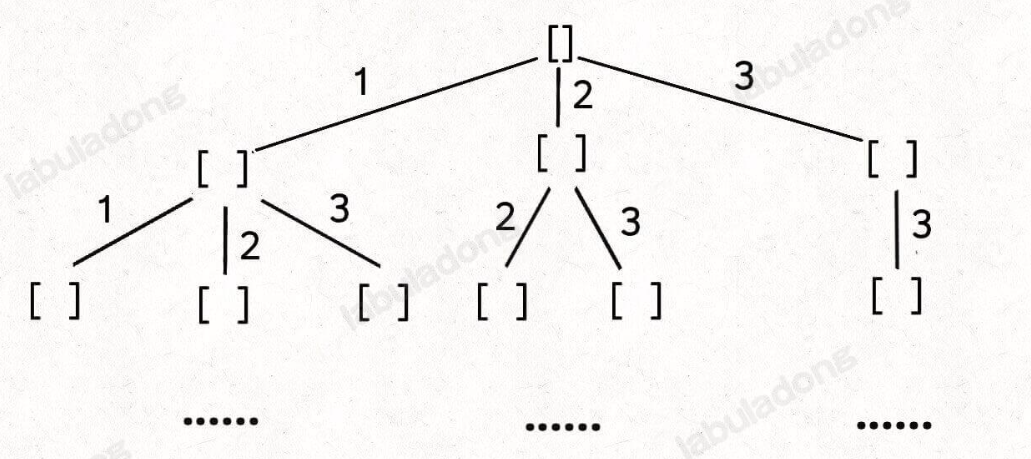
\includegraphics[width=0.5\linewidth]{pics/sub_multi}
\end{center}

	\par multi select permutation, Code is very easy, don't use used array. The time complexity is power(n, n). That is the only question which has so high time complexity. 
	


\subsubsection{Duplicate, single select}

	
	\par For combination, need to sort, then trim(prune) a branch which doesn't meet condition. 
\begin{lstlisting}
....
for (int i = start; i < len; ++i) {
	if(i>start && arr[i] == arr[i-1]) // trimming happens in these two 
	continue;                     // statements, so we need to sort first. 
	result.push_back(arr[i]);  
	sub(arr, len, i + 1, result);
	result.pop_back();
}	
....	
\end{lstlisting}

\begin{center}
	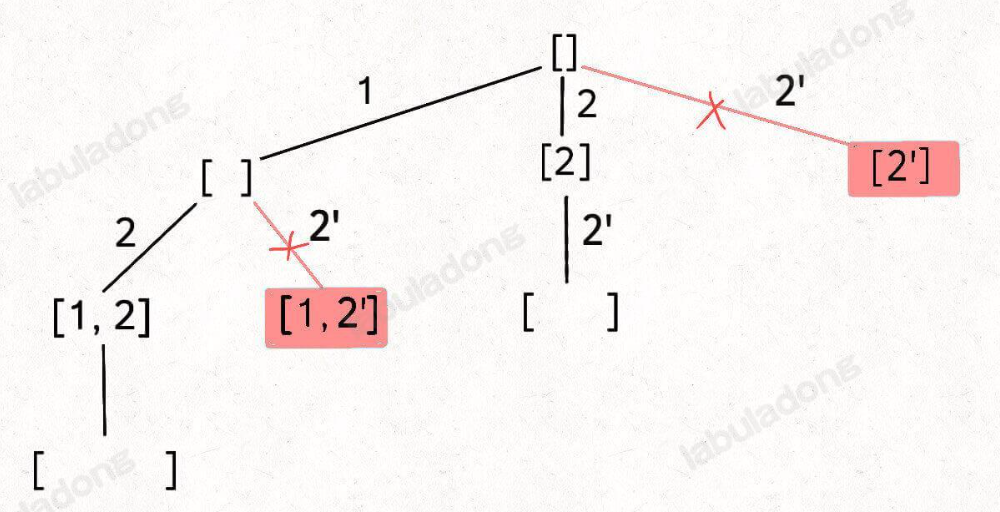
\includegraphics[width=0.5\linewidth]{pics/com_duplicate}
\end{center}
	

	\par For permutation, need to sort, then trim (prune) a branch which doesn't meet condition. 
\begin{lstlisting}
	....
	for (int i = start; i < len; ++i) {
		if(i>start && arr[i] == arr[i-1] && !used[i-1]) // trimming happens in these two 
			continue;                                // statements, so we need to sort first. 
		result.push_back(arr[i]);  
		sub(arr, len, i + 1, result);
		result.pop_back();
	}	
	....
\end{lstlisting}

	\par How to understand \verb|!used[i-1]|? 
	\begin{center}
		\includegraphics[width=0.5\linewidth]{pics/per_duplicate}
	\end{center}
	


\subsubsection{Parenthesis}

	\par The trimming idea can be applied in parenthesis problem, the basic problem is also permutation problem, but you need to trimming the branch. 
	anytime, left parenthesis should be greater or equal right parenthesis. 
	
\begin{lstlisting}
vector<string> generateParenthesis(int n) {
	vector<string> res;  //all results
	string track;
	backtrack(n, n, track, res); // left and right parenthesis number are both n
	return res;
}

void backtrack(int left, int right, string& track, vector<string>& res) {
	
	if (right < left) return; //left is less right, illegal.
	
	if (left < 0 || right < 0) return;
	// all is 0, get a legal result.
	if (left == 0 && right == 0) {
		res.push_back(track);
		return;
	}
	
	track.push_back('(');  // try to put a left 
	backtrack(left - 1, right, track, res);
	track.pop_back(); 
	
	track.push_back(')');  // try to put a right.
	backtrack(left, right - 1, track, res);
	track.pop_back(); 
}
// output is ((()))     (()())     (())()     ()(())     ()()()
\end{lstlisting}

\subsubsection{Summary}
	
	\par Four code compare: They are the most common used code template for back trace, you need to understand and 
\begin{enumerate}
	\item code 1: multi tree, call backtrace(i),  backtrace(i-1), backtrace(i-2)... This will cause a multi branch tree, and the first level has n branches, The second level has n-1 branches, untill the last level has only 1 branches.   O(n*n)
\begin{lstlisting}
	for(i ..n )
	backtrace( i+1)
\end{lstlisting}
	
	\begin{center}
		\includegraphics[width=0.5\linewidth]{pics/sub}
	\end{center}
	
	\item code 2: multi tree, on each level,  i, i-1,  i-2 backtrace O(n!)
\begin{lstlisting}
	for(j = i ..n )  // on i level, each backtrace trun (n-i) times. 
		backtrace( i+1)
\end{lstlisting}

	\includegraphics[scale=0.25]{pics/permutation.png}

	\item code 3: binary tree, global result, need reverse
	
	\item code 4: binary tree, stack partial result, don't need reverse. global result.
\end{enumerate}


\subsection{Interview questions}

	\par Eight queen
	
\begin{lstlisting}
vector<vector<string>> res;
vector<vector<string>> solveNQueens(int n) {
	
	// '.' is  void, 'Q' is queen
	vector<string> board(n, string(n, '.'));
	backtrack(board, 0);
	return res;
}


void backtrack(vector<string>& board, int row) {
	// base case
	if (row == board.size()) {
		res.push_back(board);
		return;
	}
	
	int n = board[row].size();
	for (int col = 0; col < n; col++) {
		// exclude
		if (!isValid(board, row, col)) {
			continue;
		}
		// make decision
		board[row][col] = 'Q';
		// go deeper
		backtrack(board, row + 1);
		// reverse
		board[row][col] = '.';
	}
}	
\end{lstlisting}	
	


	\par k equal subset.
	
\begin{lstlisting}
class Solution {
	public:
	bool canPartitionKSubsets(vector<int>& nums, int k) {
		int sum = accumulate(nums.begin(), nums.end(), 0);
		if (sum % k != 0) return false;
		sort(nums.begin(), nums.end(), greater<int>());
		vector<bool> visited(nums.size(), false);
		return helper(nums, k, sum / k, 0, 0, visited);
	}
	bool helper(vector<int>& nums, int k, int target, int start, int curSum, vector<bool>& visited) {
		if (k == 1) return true;
		if (curSum > target) return false; //return false is used to trim branch
		if (curSum == target) return helper(nums, k - 1, target, 0, 0, visited);  
		for (int i = start; i < nums.size(); ++i) {
			if (visited[i]) continue;
			visited[i] = true;
			if (helper(nums, k, target, i + 1, curSum + nums[i], visited)) return true;
			visited[i] = false;
		}
		return false;
	}
};	
\end{lstlisting}	
	

\section{Dynamic programming}
\subsection{Basic Idea}
	
	\par The basic question can be asked: can(bool), min or count(one number), all(list or vector). \textbf{Usually, can and all can be used backtracking algorithm, but man/min is a typical indication of greed or dynamic programming.}
	
	\par The difference between dynamic programming and greedy algorithms is that with dynamic programming, the sub-problems overlap. That means that by memorizing" solutions to some sub-problems, you can solve other sub-problems more quickly. 
	
	\par Three key words in dynamic programming are: state, transition and choice. state is most time defined by question directly,  the most difficult question is \textbf{How the current states is transitioned through choices from previous states, which is the transition equation}. If the state is defined in terms of the problem and you find it difficult to write the transition equation, then you must redefine the state; one example is Given an integer array nums, find the 
	subarray with the largest sum, and return its sum. (https://leetcode.com/problems/maximum-subarray/description/)
	
	
	\par The top-down approach is generally recursive (but less efficient) and more intuitive to implement as it is often a matter of recognizing the pattern in an algorithm and refactoring it as a dynamic programming solution.The bottom-up approach is generally iterative (and more efficient), but less intuitive and requires us to solve (and know!) the smaller problems first then use the combined values of the smaller problems for the larger solution. We refer to top-down solutions as memorization and bottom-up as tabulation.
	
	
%	\par If we don’t need to solve all the problems and are just looking for the optimal solution, memorization is better.
%	
%	\par If we do need to solve all the problems, that means we are going to make a lot of recursive calls, and tabulation is better.
	
	\par The caveat is that memorization is generally more intuitive to implement especially when we don’t know the solution to subproblems, whereas tabulation requires us to know the solutions, or bottom, in advance, in order to build our way up.
	
	\par In Divide and Conquer, the sub-problems are independent of each other while in case of Dynamic Programming, the sub-problems are not independent of each other (Solution of one sub-problem may be required to solve another sub-problem). Divide and Conquer works by dividing the problem into sub-problems, conquer each sub-problem recursively and combine these solutions. solves a problem by combining the solutions to sub-problems
	
	\begin{itemize}
		\item Partition the problem into non-overlapping sub-problems
		
		\item Solve the sub-problems recursively
		
		\item Combine their solutions to solve the original problem
	\end{itemize}
	
	
	\par Dynamic Programming is a technique for solving problems with overlapping subproblems. Each sub-problem is solved only once and the result of each sub-problem is stored in a table ( generally implemented as an array or a hash table) for future references. These sub-solutions may be used to obtain the original solution and the technique of storing the sub-problem solutions is known as memoization.
	
	\par You may think of DP = recursion + re-use
	
	
	\par The principle of optimality. No matter what the first decision, the remaining decisions must be optimal with respect to the state that results from this first decision
	Dynamic programming may be used only when the principle of optimality holds. Useful when the sub-problems are overlapping
	
	Solve an optimization problem by caching  sub-problem solutions rather than recomputing them
	
	\begin{itemize}
		\item Verify that the principle of optimality holds  \newline
		\includegraphics[scale=0.45]{pics/Recurrence.png} \newline
		
		\item Set up the dynamic-programming recurrence equations
		\item Solve the dynamic-programming recurrence equations for the value of the optimal solution
		\item Perform a traceback step in which the solution itself is constructed
	\end{itemize}
	
\subsection{Three questions}

	\par Write a function to return the minimum number of jumps to reach the end of the array (starting from the first element). Below is Min jump question
	
\begin{lstlisting}[numbers=none]
int arr[] = {1, 3, 5, 8, 9, 2, 6, 7, 6, 8, 9};

int minj(int arr[], int last){		
	if (last ==1 && arr[last]>=1){
		return 1;
	}
	
	int min = last;
	for(int i = last-1; i>=0;i--){
		if (i+arr[i]>=last){
			int step = 1+minj(arr,i);
			if( step<min){
				min = step;
			}
		}    
	}
	return min;
}		
\end{lstlisting} 		
	
	
	\par Below is getting all questions.  
\begin{lstlisting}[numbers=none]
int arr[] = {1, 3, 5, 8, 9, 2, 6, 7, 6, 8, 9};

vector<vector<int> >  minj(int arr[], int last){	
	if (last ==1 && arr[last]>=1){
		vector<int> v1 = {1};
		vector<vector<int> > v = {v1};
		return v;
	}	
	vector<vector<int> > result;
	
	int min = last;
	for(int i = last-1; i>=0;i--){
		if (i+arr[i]>=last){
			vector<vector<int> > result1 = minj(arr,i);
			for(auto e: result1){
				e.push_back(arr[i]);
				result.push_back(e);
			}
		}
	}
	return result;
}					
\end{lstlisting} 	
	
	\par below is Can questions.  
\begin{lstlisting}[numbers=none]
int arr[] = {1, 3, 5, 8, 9, 2, 6, 7, 6, 8, 9};

bool  minj(int arr[], int last){
	
	if (last ==1 && arr[last]>=1){
		return true;
	}
	
	bool result = false;
	
	for(int i = last-1; i>=0;i--){
		if (i+arr[i]>=last){
			result = true && minj(arr,i);
			if(result)
			break;
		}
	}
	return result;
}		
\end{lstlisting} 	
	
	\par Conclusion:
	\begin{itemize}
		\item can and min is little easy, min return one number, can return one bool. 
		
		\item "all" type question need return a list, because each answer is a list, so here we return vector< vector >. 
		
		\item "all" type question is suitable Top-bottom method. can and min is suitable for bottom-top method.
	\end{itemize}
	

\subsection{one dimension}
	
	\par Longest Increasing Subsequence, top bottom method. There are a lot of overlap problem, so efficient is not good.
	
\begin{lstlisting}[numbers=none]
int _lis( int arr[], int n, int *max_ref){
	if (n == 1) /* Base case */
	return 1;
	
	// 'max_ending_here' is length of LIS ending with arr[n-1]
	int res, max_ending_here = 1;
	
	/* Recursively get all LIS ending with arr[0], arr[1] ... arr[n-2]. If arr[i-1] is smaller
	than arr[n-1], and max ending with arr[n-1] needs to be updated, then update it */
	for (int i = 1; i < n; i++){
		res = _lis(arr, i, max_ref);
		if (arr[i-1] < arr[n-1] && res + 1 > max_ending_here)
		max_ending_here = res + 1;
	}
	
	// Compare max_ending_here with the overall
	// max. And update the overall max if needed
	if (*max_ref < max_ending_here)
		*max_ref = max_ending_here;
	
	// Return length of LIS ending with arr[n-1]
	return max_ending_here;
}	
\end{lstlisting}	
	
	\par Longest Increasing Subsequence, bottom-top method. There are no overlap problem, so efficiency is better.
	
\begin{lstlisting}[numbers=none]
int lis( int arr[], int n ){
	int lis[n];
	lis[0] = 1;  
	
	/* Compute optimized LIS values in
	bottom up manner */
	for (int i = 1; i < n; i++ ){
		lis[i] = 1;
		for (int j = 0; j < i; j++ ) 
		if ( arr[i] > arr[j] && lis[i] < lis[j] + 1)
		lis[i] = lis[j] + 1;
	}
	// Return maximum value in lis[]
	return *max_element(lis, lis+n);
}	
\end{lstlisting}	
	
	
	\par House robber
\begin{lstlisting}[numbers=none]
for (i ->n)
	for(j->i)
		max(dp[j]...)
\end{lstlisting}	
	
	
	\par Can target string be built by input string, top-bottom.
	
\begin{lstlisting}[numbers=none]
vector<string> input = {"ab", "abc", "cd", "def", "abcd", "ef" , "c"};
string target = "abcdef";

vector<vector<string> > ac(string target, const vector<string> & in ){
	if (target.size() == 0){
		return vector<vector<string>> {{}};
	}
	
	vector<vector<string>> last_result;
	for(auto i: input){
		if (target.find(i) == 0){
			string sub = target;
			sub.erase(0, i.size());
			vector<vector<string>> re = ac(sub, in);
			for(auto j : re){
				j.push_back(i);
				last_result.push_back(j);
			}
		}
	}
	return last_result;
}	
\end{lstlisting} 	
	
	\par How many way can target string be built by input string, top-bottom.
\begin{lstlisting}[numbers=none]
vector<string> input = {"purp", "p", "ur", "le", "purpl"};
string target = "purple";

int ac(string target, const vector<string> & in ){	
	int arr[7] = {1, 0, 0, 0, 0, 0, 0};
	for(int i = 0;i<7;i++){
		for (auto s: input){
			int length = s.length();
			if(target.substr(i, length) == s)
			{
				arr[i+length] += arr[i];
			}		
		}
	}	
	return arr[6];
}	
\end{lstlisting} 	
	


\subsubsection{conclusion}

	\par For this problem, first, decide to use one dimension dp (lis array in previous example). Then dp definition(state) should be match with your questions, here, state is the length of LIS. 
	
	\par dp and recursive use the same state. For example, dp and return value of recursive are both length of LIS.
	
\begin{lstlisting}[numbers=none]
for (i ->n) // A common template
for(j->i)
max(dp[j]...)	
\end{lstlisting}	
	

\subsection{Two dimension}

%	\par why palindrome and matrix need two dimension array. 
%\begin{lstlisting}
%for(int l = 2; l<n ; l++)
%	for(int i = 0; i<n -1;i++)
%		int j = 1+i-1 ...
%\end{lstlisting}	
%	
%	\includegraphics[scale=0.25]{pics/dp.drawio.png}
	
	
	\par The basic idea is below: 
\begin{center}
	\includegraphics[scale=0.65]{pics/two_dimension.png} 
\end{center}
	
	
	\par LCS problem 
\begin{lstlisting}[frame=single, language=c++]
/* Returns length of LCS for X[0..m-1], Y[0..n-1] */
int lcs( char *X, char *Y, int m, int n ) 
{ 
	int L[m + 1][n + 1]; 
	int i, j; 
	
	/* Following steps build L[m+1][n+1] in 
	bottom up fashion. Note that L[i][j] 
	contains length of LCS of X[0..i-1]
	and Y[0..j-1] */
	
	for (i = 0; i <= m; i++) { 
		for (j = 0; j <= n; j++) { 
			if (i == 0 || j == 0)  
			L[i][j] = 0;   
			//base case, the first row and the first column are all zero
			
			else if (X[i - 1] == Y[j - 1]) 
			L[i][j] = L[i - 1][j - 1] + 1; 
			
			else
			L[i][j] = max(L[i - 1][j], L[i][j - 1]); 
		} 
	} 
	
	/* L[m][n] contains length of LCS 
	for X[0..n-1] and Y[0..m-1] */
	
	return L[m][n]; 
} 		
\end{lstlisting}	
	
	\par minimal edit distance problem 
\begin{lstlisting}[frame=single, language=c++]
int min(int x, int y, int z) { return min(min(x, y), z); }
int editDistDP(string str1, string str2, int m, int n)
{
	// Create a table to store results of subproblems
	int dp[m + 1][n + 1];
	
	// Fill d[][] in bottom up manner
	for (int i = 0; i <= m; i++) {
		for (int j = 0; j <= n; j++) {
			// If first string is empty, only option is to
			// insert all characters of second string
			if (i == 0)
			dp[i][j] = j; // Min. operations = j
			
			// If second string is empty, only option is to
			// remove all characters of second string
			else if (j == 0)
			dp[i][j] = i; // Min. operations = i
			
			// If last characters are same, ignore last char
			// and recur for remaining string
			else if (str1[i - 1] == str2[j - 1])
			dp[i][j] = dp[i - 1][j - 1];
			
			// If the last character is different, consider
			// all possibilities and find the minimum
			else
			dp[i][j] = 1 + min(dp[i][j - 1], // Insert
			dp[i - 1][j], // Remove
			dp[i - 1][j - 1]); // Replace
		}
	}
	
	return dp[m][n];
}		
\end{lstlisting}	
	
	\par longest panlindrom subsequence (LPS)
\begin{lstlisting}[frame=single, language=c++]
// Returns the length of the longest palindromic subsequence in seq
int lps(char *str)
{
	int n = strlen(str);
	int i, j, cl;
	int L[n][n];  // Create a table to store results of subproblems
	
	// Strings of length 1 are palindrome of lentgh 1
	for (i = 0; i < n; i++)
	L[i][i] = 1;
	
	// Build the table. Note that the lower diagonal values of table are
	// useless and not filled in the process. The values are filled in a
	// manner similar to Matrix Chain Multiplication DP solution (See
	// https://www.geeksforgeeks.org/matrix-chain-multiplication-dp-8/). cl is length of
	// substring
	for (cl=2; cl<=n; cl++){
		for (i=0; i<n-cl+1; i++){
			j = i+cl-1;
			if (str[i] == str[j] && cl == 2)
			L[i][j] = 2;
			else if (str[i] == str[j])
			L[i][j] = L[i+1][j-1] + 2;
			else
			L[i][j] = max(L[i][j-1], L[i+1][j]);
		}
	}
	return L[0][n-1];
}		
\end{lstlisting}	
	
	
	\par Matrix multiply 
\begin{lstlisting}[frame=single, language=c++]
int MatrixChainOrder(int p[], int n){
	/* For simplicity of the program, one
	extra row and one extra column are
	allocated in m[][]. 0th row and 0th
	column of m[][] are not used */
	int m[n][n];
	
	int i, j, k, L, q;
	
	/* m[i, j] = Minimum number of scalar
	multiplications needed to compute the
	matrix A[i]A[i+1]...A[j] = A[i..j] where
	dimension of A[i] is p[i-1] x p[i] */
	
	// cost is zero when multiplying
	// one matrix.
	for (i = 1; i < n; i++)
	m[i][i] = 0;
	
	// L is chain length.
	for (L = 2; L < n; L++){
		for (i = 1; i < n - L + 1; i++){
			j = i + L - 1;
			m[i][j] = INT_MAX;
			for (k = i; k <= j - 1; k++){
				
				// q = cost/scalar multiplications
				q = m[i][k] + m[k + 1][j]
				+ p[i - 1] * p[k] * p[j];
				if (q < m[i][j])
				m[i][j] = q;
			}
		}
	}
	
	return m[1][n - 1];
}		
\end{lstlisting}	
	
	\par knapsack capacity
\begin{lstlisting}[frame=single, language=c++]
int knapSack(int W, int wt[], int val[], int n)
{
	int i, w;
	int K[n + 1][W + 1];
	
	// Build table K[][] in bottom up manner
	for(i = 0; i <= n; i++)
	{
		for(w = 0; w <= W; w++)
		{
			if (i == 0 || w == 0)
			K[i][w] = 0;
			else if (wt[i - 1] <= w)
			K[i][w] = max(val[i - 1] +
			K[i - 1][w - wt[i - 1]],
			K[i - 1][w]);
			else
			K[i][w] = K[i - 1][w];
		}
	}
	return K[n][W];
}		
\end{lstlisting}	
	
	\par egg drop
\begin{lstlisting}[frame=single, language=c++]
int eggDrop(int n, int k){
	/* A 2D table where entery
	eggFloor[i][j] will represent
	minimum number of trials needed for
	i eggs and j floors. */
	int eggFloor[n + 1][k + 1];
	int res;
	int i, j, x;
	
	// We need one trial for one floor and 0
	// trials for 0 floors
	for (i = 1; i <= n; i++) {
		eggFloor[i][1] = 1;
		eggFloor[i][0] = 0;
	}
	
	// We always need j trials for one egg
	// and j floors.
	for (j = 1; j <= k; j++)
	eggFloor[1][j] = j;
	
	// Fill rest of the entries in table using
	// optimal substructure property
	for (i = 2; i <= n; i++) {
		for (j = 2; j <= k; j++) {
			eggFloor[i][j] = INT_MAX;
			for (x = 1; x <= j; x++) {
				res = 1 + max(
				eggFloor[i - 1][x - 1],
				eggFloor[i][j - x]);
				if (res < eggFloor[i][j])
				eggFloor[i][j] = res;
			}
		}
	}
	
	// eggFloor[n][k] holds the result
	return eggFloor[n][k];
}	
\end{lstlisting}	
	
	\par below is dp implementation of knapsack. 
\begin{lstlisting}
int knapsack_dp() {
	int W = 10;
	int N = 5;
	int val[] = {40, 50, 100, 95, 30};
	int wt[] = { 2, 4, 2, 5, 3 };
	int dp[6][11];
	for (int i = 0; i <= N; i++) {
		for (int w = 0; w <= W; w++) {
			if (i == 0)
			dp[i][w] = 0;
			if (w == 0)
			dp[i][w] = 0;
		}
	}
	for (int i = 1; i <= N; i++) {
		for (int w = 1; w <= W; w++) {
			if (w - wt[i - 1] < 0) {
				
				dp[i][w] = dp[i - 1][w];
			}
			else {
				
				dp[i][w] = max(
				dp[i - 1][w - wt[i - 1]] + val[i - 1],
				dp[i - 1][w]
				);
			}
		}
	}
	
	for (int i = 1; i <= N; i++) {
		for (int w = 1; w <= W; w++) {
			cout << dp[i][w] << " ";
		}
		cout << endl;
	}
	
	return dp[N][W];
}
// 0 40 40 40 40 40 40 40 40 40
// 0 40 40 50 50 90 90 90 90 90
// 0 100 100 140 140 150 150 190 190 190
// 0 100 100 140 140 150 195 195 235 235
// 0 100 100 140 140 150 195 195 235 235	
\end{lstlisting}



\subsection{three dimension}
	\par A typical question is stock buy and sell. 
\begin{lstlisting}
for (int i = 0; i < n; i++) 
for (int k = max_k; k >= 1; k--) {
	if (i - 1 == -1) {
		// deal i = -1  base case
		dp[i][k][0] = 0;
		dp[i][k][1] = -prices[i];
		continue;
	}
	dp[i][k][0] = Math.max(dp[i-1][k][0], dp[i-1][k][1] + prices[i]);
	dp[i][k][1] = Math.max(dp[i-1][k][1], dp[i-1][k-1][0] - prices[i]);   // k-1 here. three dimension array, go to the next level, please refer the below picture.
}
return dp[n - 1][max_k][0];	
\end{lstlisting}	
	
\begin{center}
	\includegraphics[width=0.7\linewidth]{pics/stock.png} 
\end{center}
	

\subsection{Summary}


	\par The general form of a dynamic programming problem is to find the optimal value. Since the goal is to find the optimal value, what is the core issue? The core issue in solving dynamic programming problems is enumeration. The steps are: define the base case, clarify the "states," clarify the "choices," and define the meaning of the dp array/function. I summarize this theory as "one model with three characteristics."
	
	\par First, let's look at what "one model" refers to. It describes the model of problems that dynamic programming is suited for solving. I define this model as the "optimal solution model with multi-stage decision-making." Let me explain this in detail.
	
	\par Dynamic programming is typically used to solve optimization problems. The process of solving such problems involves going through multiple decision stages. Each decision stage corresponds to a set of states. We then search for a sequence of decisions that, when followed, results in the optimal value we seek.
	
	\par Now, let's explore what the "three characteristics" are. They are optimal substructure, no aftereffect, and overlapping subproblems. These concepts are somewhat abstract, so I'll explain them one by one:
	
	\par Optimal Substructure
	Optimal substructure means that the optimal solution to the problem contains the optimal solutions to its subproblems. In other words, we can derive the optimal solution of the problem from the optimal solutions of its subproblems. When we map optimal substructure to the dynamic programming problem model we defined earlier, it means that the states in the later stages can be derived from the states in the earlier stages.
	
	\par No after effect (or Memorylessness)
	This has two meanings. The first is that when deriving the state of a later stage, we only care about the state values of the earlier stages, not how those states were derived step by step. The second meaning is that once the state of a certain stage is determined, it is not affected by decisions made in later stages. No after effect is a relatively "relaxed" requirement. As long as the dynamic programming problem model mentioned earlier is satisfied, the no after effect property will generally hold.
	
	\par Overlapping Subproblems
	This concept is easier to understand. As mentioned several times in the previous section, in summary, it means that different decision sequences may reach the same stage, potentially resulting in repeated states.
	
		
	\par Define the base case: This is simple. Clearly, when the target amount is 0, the algorithm should return 0, because no coins are needed to reach the target amount.
	
	\par Identify the "state": This refers to the variables that change between the main problem and subproblems. Since the number of coins is unlimited and the coin denominations are given by the problem, the only variable that changes as the solution progresses toward the base case is the target amount. Thus, the only "state" is the target amount (amount).
	
	\par Determine the "choices": These are the actions that lead to changes in the state. Why does the target amount change? Because you are selecting coins. Each time you choose a coin, it effectively reduces the target amount. Therefore, all the coin denominations represent your "choices."
	
	\par Clarify the definition of the dp function/array: In this case, we're discussing a top-down approach, so there will be a recursive dp function. Generally, the function's parameters are the variables that change during state transitions (the "state"), as mentioned earlier. The function's return value is what the problem asks us to calculate. For this problem, there is only one state—the target amount—and the problem asks us to compute the minimum number of coins needed to reach the target amount.
	
	\par Of course, this isn’t strictly a dynamic programming problem. It aims to illustrate that the optimal substructure is not unique to dynamic programming; most problems that involve finding an optimal value have this property. On the flip side, if the optimal substructure property is present, it usually means you’re asked to find an optimal value. When you encounter challenging optimization problems, thinking about dynamic programming is often the right approach—that’s the pattern.
	
	Dynamic programming involves the following steps:
	
	Transform the current problem into subproblems: Once you break it down into subproblems, define the state transition equation, which explains how the solution to the current problem is derived from the combination (or transformation) of the subproblems.
	
	Decide whether to use top-down DP (subproblem, subproblem state 1, subproblem state 2, etc.) or bottom-up DP: For example, dp[subproblem], dp[subproblem state 1], dp[subproblem state 2], etc.
	
	Determine the traversal direction and base case based on the meaning of the dp function.
	
	Apply the template code to implement the solution.
	
	
	Below are some common examples: the egg-drop problem, subsequence problems and finding the minimum. The 0/1 knapsack problem and stock trading problem.
	
	Why does the n-floor egg-drop problem require considering all subproblems from 0 to i-1 for each i, while the stock trading problem only needs to consider the previous state?  One thing to note is that in the stock trading problem, k represents the maximum number of allowed transactions, not the number of transactions already completed. It’s a way of describing the state.
	
	\par \textbf(Based on the problem, define the dp, then take dp[i-1] and try to see if you can combine dp[i-1] to form dp. Generally, there are two possibilities: either it involves all previous states (as in the egg-drop problem), or it involves just the previous two states (as in the stock trading problem). The current state can transition from buying or not buying.)"
	
	
	\par Four questions: matrix multiply, shoot ballon, gambling(piles stone, take from left and right) and maxium panlinmon subsequecne. The answer is located in the top-right corner of a 2D array, and you need to use diagonal traversal or reverse traversal. The transition equations are almost identical.
	
\begin{lstlisting}
for (int i = n; i >= 0; i--) {
	// j from left to right
	for (int j = i + 1; j < n + 2; j++) {
		// "Which balloon is the last to be burst?"
		
		for (int k = i + 1; k < j; k++) {
			// choose the best option
			dp[i][j] = Math.max(
			dp[i][j], 
			dp[i][k] + dp[k][j] + points[i]*points[j]*points[k]
			);
		}
	}
}	
\end{lstlisting}	
	
	\par Two questions: Regular expressions and edit distance: The result is in the bottom-right corner, and a forward traversal is needed. The subfunction represents an edit or match operation.
\begin{lstlisting}
bool dp(string& s, int i, string& p, int j) {
	if (s[i] == p[j] || p[j] == '.') {
		// match
		if (j < p.size() - 1 && p[j + 1] == '*') {
			// 1.1 regex match 0 or more
			return dp(s, i, p, j + 2)
			|| dp(s, i + 1, p, j);
		} else {
			// 1.2 normal match 1 
			return dp(s, i + 1, p, j + 1);
		}
	} else {
		// not match 
		if (j < p.size() - 1 && p[j + 1] == '*') {
			// 2.1 regex match 0 times
			return dp(s, i, p, j + 2);
		} else {
			// 2.2 can't continue match
			return false;
		}
	}
}

// return s1[0..i] and s2[0..j] minimum edition distance
int dp(String s1, int i, String s2, int j) {
	// base case
	if (i == -1) return j + 1;
	if (j == -1) return i + 1;
	
	if (s1.charAt(i) == s2.charAt(j)) {
		return dp(s1, i - 1, s2, j - 1); // do nothing
	}
	return min(
	dp(s1, i, s2, j - 1) + 1,    // insert
	dp(s1, i - 1, s2, j) + 1,    // delete
	dp(s1, i - 1, s2, j - 1) + 1 // replace
	);
}		
\end{lstlisting}	
	

\begin{lstlisting}	
for (int i = 1; i <= n; ++i) {
	for (int j = 1; j <= min(i, m); ++j) {
		if (j == 1) {
			dp[i][j] = sum[i];
		} else {
			for (int k = 1; k <= i - 1; ++k) {
				dp[i][j] = min(dp[i][j], max(dp[k][j - 1], sum[i] - sum[k]));
			}
		}
	}
}
return dp[n][m]	
\end{lstlisting}	
	

	


\section{Branch and bound}

	\par \textbf{Backtracking mainly use BFS, not DFS.} 
\begin{itemize}
\item It is used to find all possible solutions available to the problem.

\item It traverse tree by DFS(Depth First Search).

\item It realizes that it has made a bad choice \& undoes the last choice by backing up.

\item It search the state space tree until it found a solution.

\item It involves feasibility function.
\end{itemize}


	\par Branch-and-Bound
\begin{itemize}
\item It is used to solve optimization problem.

\item It realizes that it already has a better optimal solution that the pre-solution leads to so it abandons that pre-solution.

\item It completely searches the state space tree to get optimal solution.

\item It involves bounding function.

\item Searches a solution space that is often organized as a tree (like backtracking)

\item Usually searches a tree in a breadth-first / least-cost manner (unlike backtracking)

\end{itemize}

	\par Difference between DFS and backtracking is:
\begin{itemize}
\item Backtracking is a more general purpose algorithm. Depth-First search is a specific form of backtracking related to searching tree or graphic structures. 
 
\item For a problem, solution space can be described as a tree or graphic structure, such as 0/1 backpack problem. at this time, backtracking use DFS to search the answer space, and use questions related condition to prune the sub-tree and com back. So in this way, you can think backtracking = DFS + prune. 
\end{itemize}

\par Difference between branch-bound  and backtracking is about size

\begin{itemize}
\item backtracking use stack and only add one child each time, so it use less memory compared with branch-bound

\item branch-bound store all possible child in queue, so if answer is near root, it will find answer quickly. 

\item win in size, but lose in time. backtracking will 1) find answer slower if answer is near the root, 2) branch-bound will find optimal answer. 
\end{itemize}

	\par Below I present three different methods to resolve 0-1 back pack problem. dp only can deal with integral weight. but branch-bound can deal with float value. This code can run and print out all the value, it can help you to understand the idea behind these two important algorithms. 

\par below is knapSack recursive implementation, it's also backtracking, different with using stack. The idea is same, you can see the code is simpler. 
\begin{lstlisting}
int knapSack(int W, int wt[], int val[], int n){
	if (n == 0 || W == 0) // Base Case
	return 0;
	
	// If weight of the nth item is more
	// than Knapsack capacity W, then
	// this item cannot be included
	// in the optimal solution
	if (wt[n - 1] > W)
	return knapSack(W, wt, val, n - 1);
	
	//There are two options, so there's no need to write a for-loop. Based on the options, change the state, pass the state into the recursive call, and take the maximum of the returned results.
	
	// Return the maximum of two cases:
	// (1) nth item included
	// (2) not included
	else
	
	return max(
	val[n - 1]
	+ knapSack(W - wt[n - 1], 
	wt, val, n - 1),
	knapSack(W, wt, val, n - 1));
}			
\end{lstlisting}	
	  
\begin{lstlisting}
// Structure for Item which store weight and corresponding value of Item
struct Item{
	float weight;
	int value;
};
// Node structure to store information of decision tree
struct Node{
	// level  --> Level of node in decision tree (or index in arr[]
	// profit --> Profit of nodes on path from root to this node (including this node)
	// bound ---> Upper bound of maximum profit in subtree of this node/
	int level, profit, bound;
	float weight;
};
// Comparison function to sort Item according to val/weight ratio
bool cmp(Item a, Item b){
	double r1 = (double)a.value / a.weight;
	double r2 = (double)b.value / b.weight;
	return r1 > r2;
}

// below is knapsack backtracking implementation.
int knapsack_back(int W, Item arr[], int n){
	sort(arr, arr + n, cmp); // sorting Item on basis of value per unit weight.
	
	stack<Node> S; // make a queue for traversing the node
	Node u, v;
	
	u.level = -1; // dummy node at starting
	u.profit = u.weight = 0;
	S.push(u);
	
	// One by one extract an item from decision tree compute profit of all 
	// children of extracted item and keep saving maxProfit int maxProfit = 0;
	while (!S.empty()){
		u = S.top();
		S.pop();
		// If it is starting node, assign level 0
		if (u.level == -1)
			v.level = 0;
		
		// If there is nothing on next level
		if (u.level == n - 1)
			continue;
		
		// Else if not last node, then increment level,
		// and compute profit of children nodes.
		v.level = u.level + 1;
		
		// Do the same thing,  but Without taking the item in knapsack
		v.weight = u.weight;
		v.profit = u.profit;
		S.push(v);
			
		// Taking current level's item add current level's 
		// weight and value to node u's weight and value
		v.weight = u.weight + arr[v.level].weight;
		v.profit = u.profit + arr[v.level].value;
		if(v.weight>W)
			continue;
		
		// If cumulated weight is less than W and profit 
		// is greater than previous profit, update maxprofit
		if (v.weight <= W && v.profit > maxProfit)
			maxProfit = v.profit;
			
		// If bound value is greater than profit, 
		// then only push into queue for further consideration
		S.push(v);
	}
	return maxProfit;
}

//------------------------------------------------------------------
// Returns bound of profit in subtree rooted with u.
// This function mainly uses Greedy solution to find
// an upper bound on maximum profit.
int bound(Node u, int n, int W, Item arr[]){
	// if weight overcomes the knapsack capacity, return 0 as expected bound
	if (u.weight >= W)
		return 0;
	
	// initialize bound on profit by current profit
	int profit_bound = u.profit;
	
	// start including items from index 1 more to current item index
	int j = u.level + 1;
	int totweight = u.weight;
	
	// checking index condition and knapsack capacity condition
	while ((j < n) && (totweight + arr[j].weight <= W)){
		totweight += arr[j].weight;
		profit_bound += arr[j].value;
		j++;
	}
	// If k is not n, include last item partially for  upper bound on profit
	if (j < n)
		profit_bound += (W - totweight) * arr[j].value / arr[j].weight;
	return profit_bound;
}

// Returns maximum profit we can get with capacity W
int knapsack_bb(int W, Item arr[], int n){
	// sorting Item on basis of value per unit weight.
	sort(arr, arr + n, cmp);
	queue<Node> Q; 	// make a queue for traversing the node
	Node u, v;

	u.level = -1;  // dummy node at starting
	u.profit = u.weight = 0;
	Q.push(u);
	
	// One by one extract an item from decision tree compute
	// profit of all children of extracted item and keep saving maxProfit
	int maxProfit = 0;
	while (!Q.empty()) {
		u = Q.front();
		Q.pop();
		if (u.level == -1)
			v.level = 0;
		
		// If there is nothing on next level
		if (u.level == n - 1)
			continue;
			
		// Else if not last node, then increment level,
		// and compute profit of children nodes.
		v.level = u.level + 1;
		
		// Taking current level's item add current level's 
		//weight and value to node u's weight and value
		v.weight = u.weight + arr[v.level].weight;
		v.profit = u.profit + arr[v.level].value;
		
		// If cumulated weight is less than W and profit 
		// is greater than previous profit, update maxprofit
		if (v.weight <= W && v.profit > maxProfit)
			maxProfit = v.profit;
		
		// Get the upper bound on profit to decide whether to add v to Q or not. If bound value 
		//is greater than profit, then only push into queue for further consideration
		v.bound = bound(v, n, W, arr);
		if (v.bound > maxProfit)
			Q.push(v);
		
		// Do the same thing,  but Without taking the item in knapsack
		v.weight = u.weight;
		v.profit = u.profit;
		v.bound = bound(v, n, W, arr);
		if (v.bound > maxProfit)
			Q.push(v);
	}
	return maxProfit;
}
int main(){
	int W = 10;   // Weight of knapsack
	Item arr[] = { {2, 40}, {3.14, 50}, {1.98, 100}, {5, 95}, {3, 30} };
	int n = sizeof(arr) / sizeof(arr[0]); //n object.
	
	knapsack_back(W, arr, n); //use backtracking 	
	knapsack_bb(W, arr, n); //use branch and bound
}
\end{lstlisting}
\par Below figure illustrates the backtracking
\begin{center}
	\includegraphics[scale=0.85]{pics/ks_bt.png}
\end{center}

\par Below figure illustrates the branch and bound
\begin{center}
	\includegraphics[scale=0.85]{pics/ks_bb.png}
\end{center}


\par Recursive 0-1 pack pack. This is back trace, but why don't we have reverse decision? because in eight queen, we use reference parameter pass it to function(all function share). Here, we use stack, in each level, we have saved the local variable( you can think that it has been reversed by poping stack.)  That is the difference.  Another important thing is that for 0-1 pack and eight queen,  we need a logically recursive tree. So we need to simulate a "level" conception.  \textbf{0-1 pack stack solution, we save level information to the each node. 0-1 recursive solution, we use int i (array index)as level information. in eight queen, we use row information as level information }. level is the level information in the recursive solution tree.  
\begin{lstlisting}
public int maxW = Integer.MIN_VALUE; 
// cw current weight, i: current item call with f(0, 0, a, 10, 100)
public void f(int i, int cw, int[] items, int n, int w) {
	if (cw == w || i == n) { // cw==w is full or select all items
		if (cw > maxW) maxW = cw;
		return;
	}
	f(i+1, cw, items, n, w);
	if (cw + items[i] <= w) {// bigger than w, give up
		f(i+1,cw + items[i], items, n, w);
	}
}
\end{lstlisting}


%	\par A example can be see in ref PPT. Container and ship problems. 
	
\section{Summary}

	\par \textbf{The most import rule:} Break the big problem down into atomic problems. If the atomic problem requires some global conditions, then include the necessary data and data structures. Write the logic to handle this atomic problem (you may need to use a if..else to handle different conditions inside this atomic problem). Then apply this atomic problem handling logic into \textbf{recursion} or \textbf{iteration}. Difference between recursive and iterate.
	
	\begin{itemize}
		\item Recursive: Simple, intuitive code unless care is taken to avoid recomputing previously computed values, the recursive program will have prohibitive complexity
		
		\item Iterative: Not require additional space for the recursion stack. To minimize run time overheads, and hence to reduce actual run time, dynamic programming recurrences are almost always solved iteratively. (no recursion).
	\end{itemize}
	

\begin{center}
	\includegraphics[scale=0.50]{pics/rule.drawio.png}
\end{center}

	\par Difference between backtracking and DP:
	\begin{itemize}
		\item Both backtracking and dynamic programming involve a series of decisions. The difference is that in backtracking, certain constraints must be satisfied during the decision-making process (such as in the N-Queens problem). If the constraints are not met, you need to undo that decision. Dynamic programming, on the other hand, deals with the global optimal solution. So for each decision, you typically compare and record the optimal solution for the subproblem in order to eventually derive the global optimal solution.
		
		\item Another difference is that backtracking often uses recursion, while dynamic programming uses iteration (usually over a 2D array). However, sometimes the two approaches can be combined, such as in the partition problem, where backtracking is primarily used, but you can also record solutions to subproblems (using dynamic programming techniques) to reduce the number of recursive calls.
		
		\item typical question for DP is stock buy and sell k time.  typical question for backtrack is k equal subset. They all involve extra k parameter. With k parameter, you can think that it's k level, on each level, there is tree or array structure. That is the most complex problem you can meet in the interview questions. With k, you can think it's multi layer, for back track, each layer has a tree (k equal subset). For dp, each layer has two dimension array.

\begin{center}
	\includegraphics[scale=0.45]{pics/dp_back.drawio.png}
\end{center}

		
	\end{itemize}
	
	  
\chapter{Interview preparation}


\section{Coding tips and traps}
\par Pay more attention to below points when you write C++ code:
\begin{itemize}
	\item for vector and array, pay attention to size-1 is the last index. also stick to left close and right ).  size/2 is what index?  
	
	\item Check variable name. 
	
	\item Return in lambda and recursive. 
	
	\item  Check if miss ; in the endl
	
	\item Add () if expression is complicated. 
	\item Pay left edge (0) and right edge ( last element)
	\item Understand index and length. 
\begin{lstlisting}
while(index<length)
\end{lstlisting}	
	\item When while exist, understand index position and what it represent?
	\item use auto as possible.
	
	\item if you want to loop from length to 0, index must be int. can't be size\_t, otherwise, --index will never small than 0. (Must remember)
	
	\textbf{Most of complex data structure need hash and list combine.}
	
	\item \textbf{try you best to write zero bug code}
\begin{lstlisting}
A fun(B)   //must have return type
{
	C;      //must have ;
	return //must have return statment
}	

class A{
	public: //must have public, private
};  //must have ; here.	
\end{lstlisting}	
	
	
\end{itemize}

\subsection{famous question}

	\par leetcode 263, 292, 463, 530 561, 572. 680, 696, 700, 766, 821, 942,  (change serial equal to adjacent equal ) need to come back to learn. 1037, 1071, 1078, leetcode 1184 

%\subsection{array}
%\begin{itemize}
%	\item LEADER, Next Greater Element. Number of incursion.
%\end{itemize}

\section{Code template}

	\par You need to remember some famous algorithms implementation:
\begin{itemize}
	\item reverse link-link
	
	\item partition and partition\_if, use slow and fast pointer and swap.
	
	\item remove and unique, use slow and fast pointer.
	
	\item find inserting point and sqrt(x) use mid=l+(r-l)/2
	
	\item find element, and left/right boundary, use binary search, left close and right close.
	
	\item reverse, two poitners and swap
	
	\item rotate, three reverse. 
	
	\item insertion sort, std::upper\_bound and std::rotate.
	
	\item nth\_element, quick select.
	
	\item sort, quick sort, merge sort and heap sort.
	
	\item inplace merge.
\end{itemize}
	

	\par sliding windows. 
	
\begin{lstlisting}
int left = 0, right = 0;

while (right < s.size()) {
	window.add(s[right]); // increase windows
	right++;
	***  //put you logic here.
	
	//anytime you increase window, check condition. 
	while (window needs shrink) {
		// reduce windows.
		window.remove(s[left]);
		left++;
		*** //put your logic here. 
	}
}

//1) only use right <s.size as main loop
//2) "windows nees shrink" condition need to be customized. 
//3) modify "window.add" and *** to your own logic. 
//4) both left and right increments ++	
\end{lstlisting}	
	
	\par When writing the backtrack function, you need to maintain the "path" that has been traversed and the current "list of available choices." When the "termination condition" is triggered, add the "path" to the result set.
	
\begin{lstlisting}
result = []
def backtrack(path , "list of avaiable choices"):
if (meet condition)
	result.add(path)
	return

for choic in "list of avaiable choices":{
	choose choice;
	backtrack(path , "maybe new list of avaiable choices");
	revoke choice;
}		
\end{lstlisting}	
		
	\par DFS and BFS code. For BFS, when D.pop we don't judge if it's visisted.  For all next current, visit them all and push them into the D. That is the difference with DFS.
\begin{lstlisting}
DFS(start){
	S.push(start)  
	while(!S.empty()){
		current = S.pop
		if(unvisited(current){
			visit current.
			for all(next to current and unvisited)
			S.push(next);
		}
	}
}		
\end{lstlisting}	
	
\begin{lstlisting} 
BFS(start){
	D.push(start)  
	while(!D.empty()){
		current = D.pop  //2) no if here
		for all(next to current and unvisited){
			visit current.  //1) push and visit at the same time. 
			D.push(next);
		}
	}
}	
\end{lstlisting}	
	
	
	\par A implementation of push\_back in \texttt{std::vector} based on \texttt{std::unique\_ptr}. 
	
\begin{lstlisting}[numbers=none]
template <typename T>
void vector<T>::push_back(const T& value){
	cout<<"call push_back"<<endl;
	if(index_>=capacity_){
		capacity_ *=2;
		cout<<"new capacity"<<endl;
		unique_ptr<int[]> temp = make_unique<T[]>(capacity_);
		T* ps = data.get();
		copy(ps, ps+capacity_, temp.get()); //That is content copy
		data = std::move(temp); //That is uni_pointer copy
	}
	data[index_] = value;
	index_++;
}			
\end{lstlisting}	
	
%		\par Reverse link list, recursive. In line 1, reference to pointer is OK, pointer to reference is illegal. use here to set \texttt{new\_head} value
%	\begin{lstlisting}[frame=single, language=c++]	
%		void rev(Node* pre, Node* head, Node* & new_head ){ 
%			if(head == NULL){
%				new_head = pre;
%				return; //don't forgot return here. 
%			}
%			cout<<head->data<<" "<<endl;
%			Node* next = head->next;
%			head->next = pre;
%			rev(head, next, new_head);
%		}	
%	\end{lstlisting}
%	
%	
%		\par Fast and slow pointer in linklist.	
%	\begin{lstlisting}[frame=single, language=c++]	
%		while (fast_ptr != NULL && fast_ptr->next != NULL) {
%			fast_ptr = fast_ptr->next->next;	
%			/*We need previous of the slow_ptr for linked lists with odd elements */
%			prev_of_slow_ptr = slow_ptr;
%			slow_ptr = slow_ptr->next;
%		}
%		
%		/* fast_ptr would become NULL when there are even elements in list.And not 
%		NULL for odd elements. We need to skip the middle node for odd 
%		case and store it somewhere so that we can restore the original list*/
%		if (fast_ptr != NULL) {
%			midnode = slow_ptr;
%			slow_ptr = slow_ptr->next;
%		}		
%	\end{lstlisting}
	
	
%	\item double pointers, remove 0
%
%\begin{lstlisting}
%int arr[8]= {1, 2, 0, 2, 0, 3, 0, 4};
%
%int i , j = 0;
%while(j<8){
%	if(arr[j] == 0){
%		i = j;
%		break;
%	}
%	j++;
%}
%
%while(j<8){
%	if(arr[j]!=0){
%		std::swap(arr[i], arr[j]);     
%		i++;
%	}
%	j++;
%}
%\end{lstlisting}



	
%\par BFS
%\begin{lstlisting}
%int matrix[3][3] = {{1,2, 3},
%	{4, 5, 6},
%	{7, 8, 9}};
%
%int used[3][3];  //if this node has been visited.
%
%	
%	for(int i = 0;i<3;i++)
%		for(int j = 0;j<3;j++)
%			used[i][j] = 0;
%	
%	queue<pair<int, int> > q;
%	cout<<matrix[0][0]<<endl;
%	used[0][0] = 1;
%	q.push(make_pair(0,0));
%	while(!q.empty()){
%		auto node = q.front();
%		q.pop();              //All the nodes in queue have been visited. 
%		auto i = node.first;
%		auto j = node.second;
%		
%		if(i<2 && used[i+1][j] == 0){  //before push to queue, need to judge if visited.
%			
%			cout<<matrix[i+1][j]<<endl;  //push and visit, that is the BFS requirement.
%			used[i+1][j] = 1;
%			q.push(make_pair(i+1, j));
%		}
%		if(j<2 && used[i][j+1] == 0)
%		{
%			cout<<matrix[i][j+1]<<endl;
%			used[i][j+1] = 1;
%			q.push(make_pair(i, j+1));
%		}
%		if(i>0 && used[i-1][j] == 0)
%		{   
%			cout<<matrix[i-1][j]<<endl;
%			used[i-1][j] = 1;
%			q.push(make_pair(i-1, j));
%		}
%		if(j>0 && used[i][j-1] == 0)
%		{
%			cout<<matrix[i][j-1]<<endl;
%			used[i][j-1] = 1;
%			q.push(make_pair(i, j-1));
%		}
%	}
%
%\end{lstlisting}
%
%\par dfs
%\begin{lstlisting}
%stack<pair<int, int> > s;
%s.push(make_pair(0,0));
%while(!s.empty()){
%	auto node = s.top();
%	auto i = node.first;
%	auto j = node.second;
%	if(used[i][j]!=1){   //different with BFS,  dfs also need to check if visited before visit
%		cout<<matrix[i][j]<<endl;
%		used[i][j] = 1;
%	}
%	if(i<2 && used[i+1][j] == 0)   //use if else, in the last, use pop
%	s.push(make_pair(i+1, j));
%	else if(j<2 && used[i][j+1] == 0)  // just like pre order traversal, first left tree, then right tree.
%	s.push(make_pair(i, j+1));
%	else if(i>0 && used[i-1][j] == 0)
%	s.push(make_pair(i-1, j));
%	else if(j>0 && used[i][j-1] == 0)
%	s.push(make_pair(i, j-1));
%	else
%	s.pop();	
%}
%return 0;		
%\end{lstlisting}

\par Best sell problem, 

\begin{lstlisting}
std::array<int, 9> arr = {2, 3, 8, 100, 20, 1, 1, 2, 1 };
std::unordered_map<int, int> dic;
for(auto e: arr)
{
	dic[e]++;  //don't need find
}

std::vector< std::pair<int, int> > data( dic.begin(), dic.end() );  //build vector directly.

std::partial_sort( data.begin(), data.begin()+2, data.end(), [](auto &e1, auto &e2){return e1.second>e2.second;}); 
                                       //use lambda to descend order. 

for(auto &e: data){
	cout<<e.first<<"--->"<<e.second<<endl;
}	
\end{lstlisting}


\section{Typical interviwe questions}
\subsection{data structure}
\subsubsection{array}
\begin{itemize}
	
	\item maximum difference from right element( one time stock buy and sell), 
	
	\item circular queue, three points: 1) empty, 2) full and 3) front+1/length = rear. 
	
	
	\item stock one buy ans sell
	\item next larger (leader problem) (mono stack)
	\item maximum sliding window(mono queue)
	\item partial sum used for random select with weight. 
	
	\item heap (child-1)/2 is parent.  Parent*2+1 is left child, parent*2+2 is right child. If you forget, just remember three element, 0, 1, 2, then  (2-1)/2 =0 , but 2/2 = 1, that is not correct. 
	
	
\end{itemize}

\subsubsection{list}
\begin{itemize}
	\item reverse link list
	\item judge if there is loop, where is the entry of loop? 
\end{itemize}

\subsubsection{tree}
\begin{itemize}
	\item LCA, (How to resolve if only one node is here? )
	\item Judge if tree is valid BST? (how to understand min and max) 
	\item Number of BST?  
	\item Build tree from serialize
	\item delete node if path sum < k
\end{itemize}

\subsubsection{graph}

\begin{itemize}
	\item union-find aglorithm and use this to find spanning tree.
	
\end{itemize}

\subsection{algorithms}
%\subsubsection{interval}
%\begin{itemize}
%	\item one meeting room and minimum meeting rootm (need end sort.)
%	\item delete overlap interval
%	\item combine overlap interval.
%	\item video combine, 
%\end{itemize}

\subsubsection{two pointers-slow and fast}
	\par duplicate and partition

\subsubsection{two pointers-sliding windows}
	\par leetcode 76. Minimum Window Substring

\subsubsection{D\&C}
	\par nth element, find rotate, and left boundary. These three methods has different left and right boundary.  In these method, we usually input first index and last index (not size of array), and also left close, right close interval, this makes programming a little easier. 
	
	\par A variant is index is in the middle. these questions includes all parenthesis, child tree and matrix mulitplication.
\begin{lstlisting}
fun( int l, int r)

for(int k = l ;k<r; k++){
	fun( l,k);
	fun( k, r)
}			
\end{lstlisting}	

\subsubsection{binary search}
	\par 1) money eat banana 
	
\subsubsection{Backtracking}

	\par Some common examples:  1) permutation, subset and combination. Knapsack problem. 2) Legal parentheses combination. 3) The most complicated example is k equal subset problem. 



\section{Project}
\begin{itemize}
	\item drop of knowledge C++, sixth edition. includes all modern C++ 17/20 features. Such as move semantic,  smart pointer, concurrency, brace initialization and generic programming. 
	
	\item A compiler project. Intermediate representation, Whirl to LLVM. 
	
	\item A Trade Repository or Swap Data Repository is an entity that centrally collects and maintains the records of over-the-counter (OTC) derivatives. CFTC. Commodity Futures Trading Commission.   Athena is a cross-asset platform transforming technology at JP Morgan. It delivers innovative and efficient applications to a wide range of the firm's businesses, including sales, trading, operations, risk and research. Athena combined the best of open source technologies
	
	\item There are two main types of RFID tags: battery-operated and passive. 
	
	
	\item Tell me about a time you worked hard at something but the end result was unsuccessful. Why? What did
	you learn?
	
	UH64 is a C++ compiler with its own intermediate representation (IR) called WHIRL. Clang, a highly successful commercial C++ compiler, uses LLVM as its IR. My role in the project was to convert WHIRL to LLVM. The goal was to extend LLVM’s support for more CPUs while leveraging WHIRL’s optimizations in certain areas, combining the strengths of both.
	
	The main challenge was the large codebase, which consists of 4 million lines of code. To address this, I focused primarily on the IR domain. I also used a powerful IDE called Understand, which helps analyze source code quickly and efficiently.
	
	\item What was the most demanding or time-consuming project or initiative in your recent work experience?
	
	We need to submit reports to the CFTC within 15 minutes, or we face a fine of \$15 per transaction. Initially, we used a single server for this task, but due to the volatility of the FX market, which is influenced by politics, we decided to deploy an additional server.
	
	The reporting system is developed in Python, but since Python doesn’t handle concurrency well, we implemented multiprocessing. To manage synchronization, we also used a database. Additionally, we developed algorithms to make the system scalable, similar to a simple Kubernetes setup.
	
	The results were positive. Each year, the CFTC provides a statistical report on all major banks, and JPMorgan ranked number one, with 98\% of transactions being reported within 15 minutes.
	
	\item Can you tell me how you discovered a hidden requirement or non-obvious outcome in a recent project?
	
	move the bar to open the lid. But the bar 
	
	\item Share an example of when you changed a design approach because of someone else’s input/better idea?
	
	
	
	
	\item Can you describe a time when you were stuck on a project or solution?
	
	Double-free errors are very challenging to debug, especially in embedded applications. I attempted to use tools like Valgrind, but it wasn’t supported in this environment. I also tried implementing a custom new operator, but it wouldn’t compile successfully.
	
	After reviewing the source code, I discovered that both processes were using the same thread pool. I resolved the issue by switching to a shared\_ptr, which fixed the memory problem. I was stuck on this for almost two weeks, but now I feel very confident in handling any memory-related issues, even in highly constrained environments.
	
	
	\item In the most recent case where a team member suggested a change that you disagreed with, what steps did
	you take to reach a resolution?
	
	I will develop a test case to approve my stand point view. Stop talking, Show me the source code. 
	
	\item Vizio was acquired by Walmart and is currently undergoing a transformation, outsourcing technical work to offshore teams while focusing on the advertising business. I’ve been moved to developing GUI apps and interfaces, which doesn’t allow me to fully use my skills in low-level algorithms and C++. That’s why I’m looking for a new position.
	
	\item My wife is a resident doctor undergoing training at a hospital in Dallas. This is a rare opportunity and a family decision.
	
	\item I have expert-level knowledge of C/C++ and have published a book on C++ and you can purchase it from amazon website. I hold a Ph.D. and have a patent in algorithms, which enables me to handle complex algorithmic and machine learning challenges. I have experience working on a C++ compiler, giving me a strong understanding of optimization and machine code. I have many years of experience, including extensive teamwork and CI/CD expertise. I’m familiar with the entire software development process and tools, essentially making me a full-stack developer. 
	
	
\end{itemize}



\ifx \allfiles \undefined
%\end{CJK*}
\end{document}
\fi
